\documentclass[
	parspace,
	%final, % Teendők elrejtése / Set final to hide todos
]{elteikthesis}[2020/11/23]

\usepackage{pdfpages}
\usepackage{inconsolata}
\usepackage{color}

\definecolor{lightgray}{rgb}{.9,.9,.9}
\definecolor{darkgray}{rgb}{.4,.4,.4}
\definecolor{purple}{rgb}{0.65, 0.12, 0.82}


\title{Unit tesztek kódlefedettség-vizsgálata a szoftververziókban}
\date{2021}

\author{Marczinus Dávid}
\degree{Programtervező informatikus MSc}

\supervisor{Kovács Attila}
\affiliation{Hab. egyetemi docens}

\university{Eötvös Loránd Tudományegyetem}
\faculty{Informatikai Kar}
\department{Komputeralgebra Tanszék}
\city{Budapest}
\logo{elte_cimer_szines}

\BiblatexHungarianWarningOff
\addbibresource{thesis.bib}

\begin{document}

\documentlang{magyar}

% Lábjegyzet folytonos számozása fejezetek között
% Contiunous counting of footnotes among chapters
\counterwithout{footnote}{chapter}

% Tartalomjegyzék oldalszámozásának rejtése
% Hide page numbering of ToC
\newcounter{conpageno}
\let\oldtableofcontents\tableofcontents
\renewcommand{\tableofcontents}{
	\pagenumbering{gobble}
	\oldtableofcontents
	\cleardoublepage
	\setcounter{conpageno}{\value{page}}
	\pagenumbering{arabic}
	\setcounter{page}{\value{conpageno}}
}

\newcommand{\code}[1]{\texttt{#1}}

\lstdefinelanguage{JavaScript}{
	keywords={typeof, new, true, false, catch, function, return, null, catch, switch, var, if, in, while, do, else, case, break},
	keywordstyle=\color{blue}\bfseries,
	ndkeywords={class, export, boolean, throw, implements, import, this},
	ndkeywordstyle=\color{darkgray}\bfseries,
	identifierstyle=\color{black},
	sensitive=false,
	comment=[l]{//},
	morecomment=[s]{/*}{*/},
	commentstyle=\color{purple}\ttfamily,
	stringstyle=\color{red}\ttfamily,
	morestring=[b]',
	morestring=[b]"
}

\definecolor{eclipseStrings}{RGB}{42,0.0,255}
\definecolor{eclipseKeywords}{RGB}{127,0,85}
\colorlet{numb}{magenta!60!black}

\lstdefinelanguage{json}{
	basicstyle=\normalfont\ttfamily,
	commentstyle=\color{eclipseStrings}, % style of comment
	stringstyle=\color{eclipseKeywords}, % style of strings
	numbers=left,
	numberstyle=\scriptsize,
	stepnumber=1,
	numbersep=8pt,
	showstringspaces=false,
	breaklines=true,
	frame=lines,
	string=[s]{"}{"},
	comment=[l]{:\ "},
	morecomment=[l]{:"},
	literate=
		*{0}{{{\color{numb}0}}}{1}
		{1}{{{\color{numb}1}}}{1}
		{2}{{{\color{numb}2}}}{1}
		{3}{{{\color{numb}3}}}{1}
		{4}{{{\color{numb}4}}}{1}
		{5}{{{\color{numb}5}}}{1}
		{6}{{{\color{numb}6}}}{1}
		{7}{{{\color{numb}7}}}{1}
		{8}{{{\color{numb}8}}}{1}
		{9}{{{\color{numb}9}}}{1}
}

\lstset{
	basicstyle=\ttfamily\linespread{0.8},
	numberstyle=\small
}

% clear annoying hbox/vbox badness errors
\hfuzz=10000pt
\vfuzz=10000pt

\maketitle

\includepdf[pages={1}]{misc/eredet.pdf}
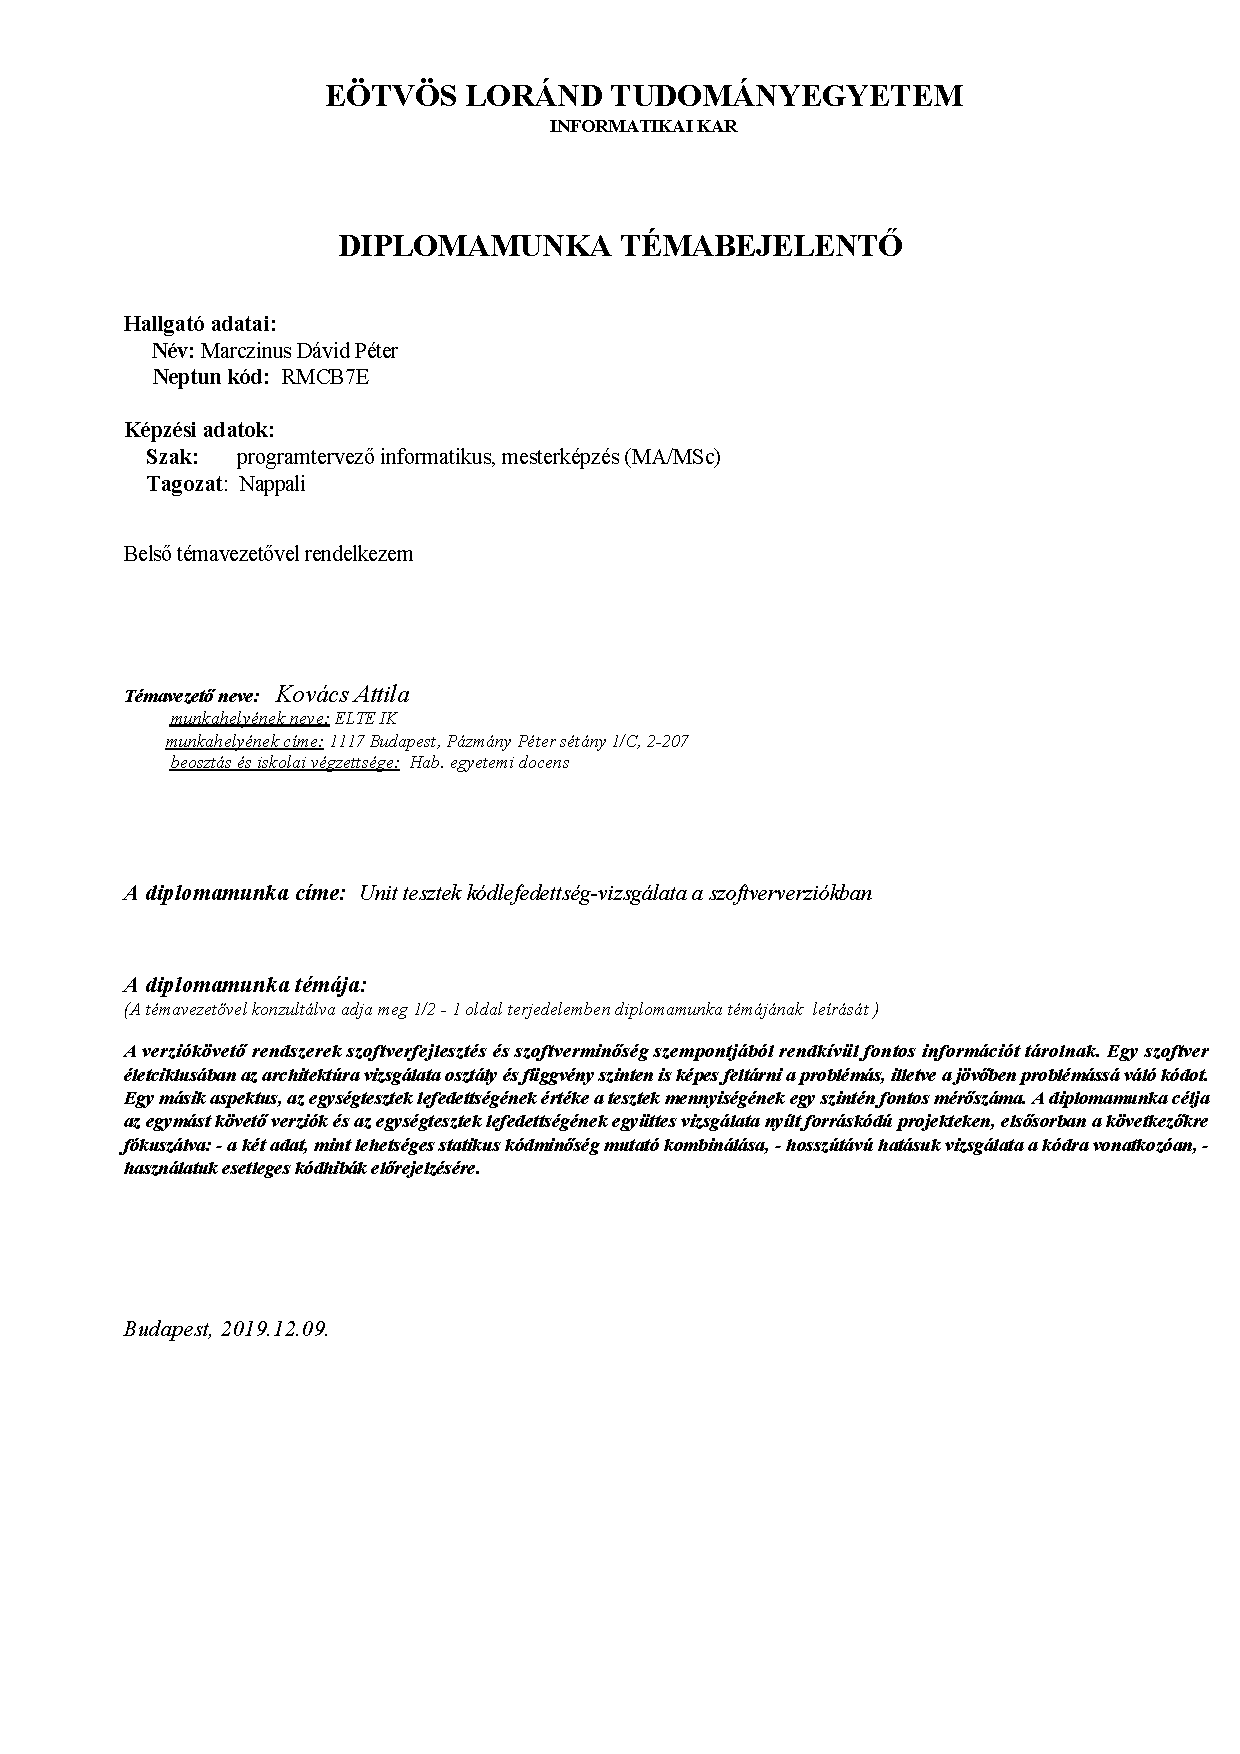
\includepdf[pages={1}]{misc/bejelento.pdf}

\tableofcontents
\cleardoublepage

\chapter{Bevezetés}
\label{ch:intro}

A modern szoftverfejlesztés egyik népszerű tautológiája, hogy minőségi, hosszú távon is karbantartható szoftvert fejleszteni nehéz. Ennek sok különböző oka, de a probléma központja az, hogy egyszerűen nehéz definiálni, hogy a "jó" és a "minőségi" szavak pontosan mit is jelentenek egy kódbázis esetében. Hiába áll közel a matematika egzakt természetéhez egy kontextus nélkül értelmezett kódsor, minél nagyobb halmazát nézzük távolról egy kódsor halmaznak, annál közelebb kerülünk a filozófiából ismerős minőség erősen homályos koncepciójához.

A tapasztalatra hivatkozhatnánk a minőség egyik prediktoraként, hiszen ha valami bevált korábban több projekten, akkor egy n+1-edik projekten is működni fog. Ez a feltételezés természetesen nem állja meg a helyét. Amellett, hogy a status quo folyamatos megkérdőjelezése előbb fog jó minőségű szoftverhez vezetni, mint annak a vak követése, azt is fontos megjegyezni, hogy egy szoftver projekt kontextusának csak egyik vektora a konkrét kód és a mögötte lévő követelmény. A fejlesztő csapat, a csapat és a csapatot alkalmazó cég kultúrája jelentősen torzítják a korábbi tapasztalat alkalmazásának hasznosságát. Melvin Conway programozó 1967-ben tett egy azóta elhíresült kijelentést, amelyre évtizedek óta csak Conway törvényeként\cite{conway} hivatkozunk:
\begin{quotation}
    Any organization that designs a system (defined broadly) will produce a design whose structure is a copy of the organization's communication structure.
\end{quotation}

Conway törvénye azt fogalmazza meg, hogy egy szervezet szoftverei jellemzően tükrözni fogják a szervezet kommunikációs struktúráját. Ez hatással van a korábban említett tapasztalati faktorra: egy szervezetben fejlesztett szoftver és a hozzá tartozó gyakorlatok nem feltétlenül illeszkednek egy másik szervezetben fejlesztett szoftver követelményeire.

Friss vezető fejlesztőként, 2019-ben futottam bele a következő kérdésbe: milyen objektív, empirikus statisztikát alkalmazhatnék egy fejlődő kódbázis elemzésére, ami mentes a saját minőségi kóddal kialakított koncepcióimtól? Ekkor futottam bele az azt megelőző évben megjelent, \textit{Software Design X-Rays}\cite{tornhillXrays} című könyvbe, ami egy számomra új, gyakorlatban hasznosítható megközelítést prezentál a kódbázisokat gyakori problémáinak felismerésére, programozási nyelvtől, paradigmától és platformtól függetlenül.

Az ötlet egyszerű: minden olyan szoftverfejlesztési projekt, ahol a minőség akármilyen szinten releváns, ott a kód verziókezelő rendszerben van tárolva. Ezek a verziókezelő rendszerek nagyon specifikus célokat szolgálnak (erről bővebben az \ref{section:version_control} szekcióban), azonban rengeteg metaadatot tárolnak a kódról projekt, fájl és sor szintjén is.

\citeauthor{tornhillXrays} két statisztikai pontra hivatkozik a könyvében:
\begin{enumerate}
    \item Egy fájl, vagy fájlban lévő sor hányszor került módosításra
    \item Egy fájl, vagy fájlban lévő sor hány különböző szerző által lett módosítva
\end{enumerate}

A feltételezés, hogy a kódbázisok problémás részein kiemelkedően magas lesz a fent említett két szám az kódbázis többi részéhez képest. Továbbá feltehető az is, hogy azok a fájlok, amiken ez megfigyelhető, azok a fejlesztés korai szakaszaitól jelen vannak és a módosítások száma a projekt életciklusa alatt nagyjából konstans marad.

Jogos kérdés lehet, hogy pontosan miért probléma az, hogy egy fájlt, illetve a benne lévő osztályt gyakran kell módosítani. Ehhez egy pillanatra hátra kell lépnünk és szót kell ejtenünk az úgynevezett code smell-ekről.

\section{Code smell}

A code smell, mint koncepció Martin Fowler \textit{Refactoring}\cite{fowlerRefactoring} című könyvével került be a programozói köztudatba. \textit{Code smell} alatt jellemzően olyan kódot értünk, aminek a működése szigorúan vett értelemben nem helytelen, azonban szoftver dizájn szempontból egészségtelen a kód hosszú távú karbantarthatóságára nézve.

Fowler a könyvében 16 különböző code smell-t definiál, amiből nekünk a következőek relevánsak:
\begin{enumerate}
    \item \textit{Long method}: szükségtelenül hosszú függvény, ami indokolatlanul sok operációt végez, nem fókuszált
    \item \textit{Large class}: indokolatlanul nagy osztály, ami reálisan több különálló osztály logikáját tartalmazza. Gyakorlatban \textit{God Class} vagy \textit{God Object} néven hivatkozunk erre a code smell-re
    \item \textit{Divergent change}: egy változtatás végrehajtásához sok, egymástól független függvény megváltoztatása szükséges
    \item \textit{Shotgun surgery}: egy kis változtatás sikeres végrehajtása csak sok osztály megváltoztatásával lehetséges
\end{enumerate}

Fontos megjegyezni, hogy a code smell, mint olyan, pusztán egy felületi heurisztika: egy kódrészlet, amire egy, vagy akár több code smell is illeszkedik, az a saját kontextusában lehet dizájn szempontból is helyes, hiszen minden szoftver projekt más. Az code smell-ek értéke abban rejlik, hogy a segítségükkel gyorsan fel tudunk ismerni gyakran előforduló problémás mintákat, majd egyéni mérlegelés után dönthetünk arról, hogy szükséges-e változtatást eszközölni a gyanús kódon.

\section{Verziókezelő}
\label{section:version_control}

A verziókezelő szerves részeit képzik a modern szoftverfejlesztésnek. A fejlesztői körökben híres \textit{Joel Test}\footnote{https://www.joelonsoftware.com/2000/08/09/the-joel-test-12-steps-to-better-code/} legelső lakmusz-tesztje, hogy egy projekt minden forráskódjának valamilyen formában verziókezelőben kell lennie, máskülönben (Spolsky véleménye szerint) a fejlesztők csak a saját és a klienseik életét nehezítik meg.

De mi is pontosan egy verziókezelő? Egy verziókezelő szoftver célja, hogy a forráskódon történő változtatások mindig világosan visszakövethetőek legyenek, egyértelműen látszódjon a változtatás előtti és utáni állapot és a forráskód akármelyik állapota akármikor elérhető és visszaállítható legyen. Fontos továbbá az is, hogy a verziókezelő rendszerek úgynevezett branch-ek használatával elősegítik, hogy egy fejlesztő csapat minden tagja képes legyen ugyanazokon a fájlokon más-más változtatásokat végrehajtani úgy, hogy a potenciálisan létrejött konfliktusokat csak egyszer kell feloldani.

Koncepcionálisan a verziókezelőket, illetve az azokban tárolt forráskódot nagyon komplex gráfként érdemes elképzelni, amelynek minden csúcsa a forráskód egy bizonyos állapota.

A legismertebb verziókezelők:
\begin{itemize}
    \item \textit{SVN}: a 2000-es évek elejének legnépszerűbb, centralizált verziókezelő rendszere.
    \item \textit{Perforce}: centralizált verziókezelő, ami koncepcionálisan az SVN-hez közelít, azonban nem nyílt forráskódú. Nagy céges környezetben a mai napig viszonylag népszerű, köszönhetően főleg annak, hogy kiválóan képes kezelni a bináris fájlokat.
    \item \textit{git}: messze a legnépszerűbb modern, decentralizált verziókezelő rendszer. Bővebben részletezve a következő szekcióban.
\end{itemize}

Terminológia szempontjából a következők lesznek fontosak:
\begin{itemize}
    \item \textit{Repository}: egy megosztott adatbázis, ami tartalmazza a verziókezelt forráskód összes különböző verziójának állapotát
    \item \textit{Commit}: változtatások egy halmaza, ami a forráskód egy korábbi változatát egy új verzióra képezi le
    \item \textit{Branch}: a forráskód egy bizonyos commit-járól való leágazás, ami egy, a szülő branch-től független commit történettel fog rendelkezni a vágási ponttól
    \item \textit{Author}: egy commit változtatásaihoz rendelt szerző
\end{itemize}

\subsection{A legnépszerűbb verziókezelő - git}\label{section:git}

A git fejlesztése 2005-ben indult Linus Torvalds vezetésével, miután a Linux kernel által használt zárt forráskódú BitKeeper verziókezelő rendszer fizetőssé vált. Ebben az érában a verziókezelő rendszerek a zárt forráskód-kiforrott funkcionalitás, nyílt forráskód-kiforratlan funkcionalitás párosok által képzett két halmazba tartoztak.

A git dizájnját a BitKeeper pozitívumai vezérlték: a merge és fork operációk legyenek egyszerűen végrehajtható műveletek, ellentétben a fő versenytársakkal, mint a CVS és az SVN, ahol többek között a materializált branch-ek nehezítették ezeket a műveleteket.

Az igazi áttörést a git-nek a 2008-ban alapított GitHub hozta meg: a 2008-as és 2014-es évek között a GitHub-on tárolt repository-k száma exponenciálisan növekedett évről évre. 2014-re a git beérte az SVN-t, 2020-ra pedig már közel háromszor annyi git-en tárolt repository-t tartott számon a nyílt forráskódú közösség, mint SVN-en.

\begin{figure}[H]
    \centering
    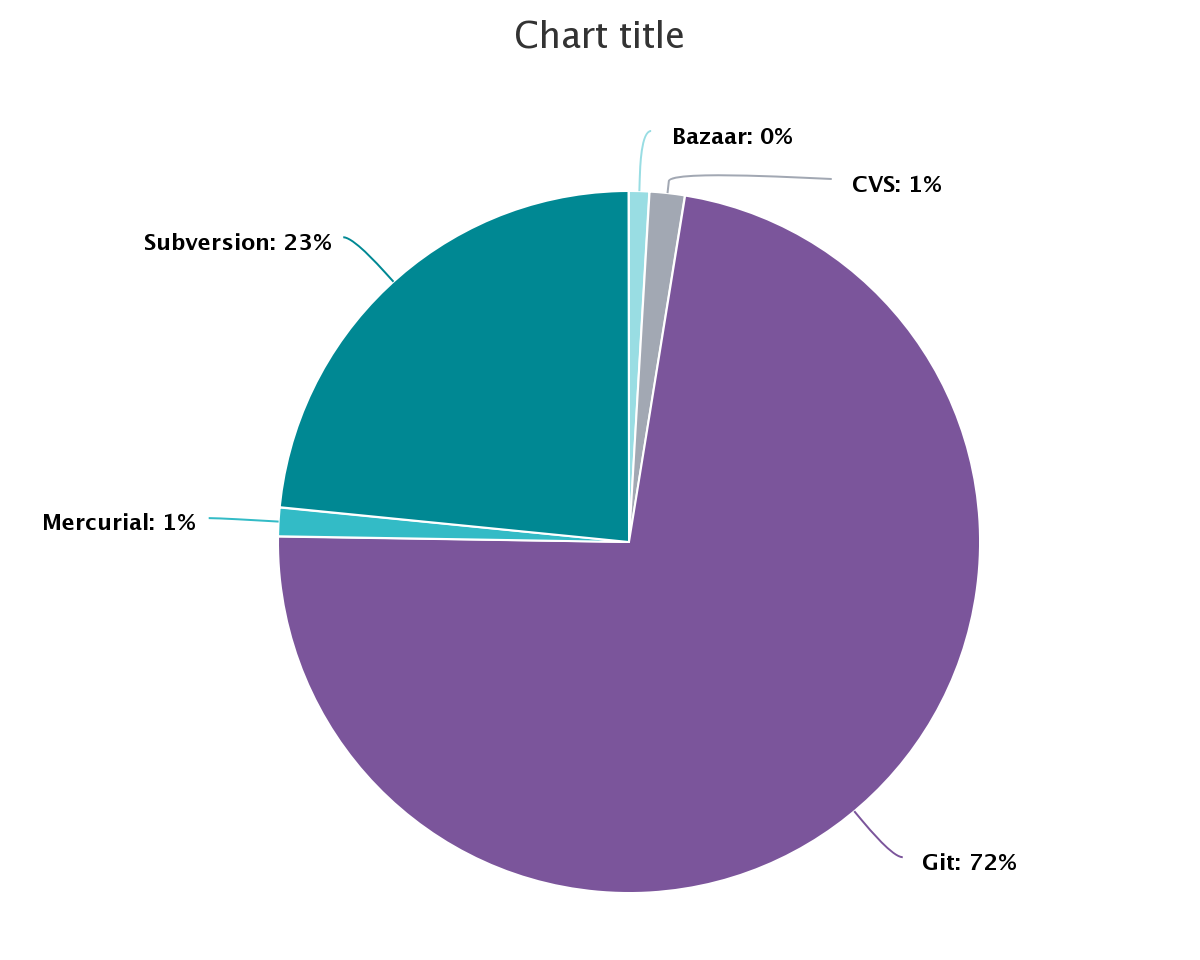
\includegraphics[width=0.8\textwidth]{images/gitMarketShare.png}
    \caption{Verziókezelők relatív népszerűsége 2020-ban}
    \label{fig:version-controls}
\end{figure}

\begin{figure}[H]
    \centering
    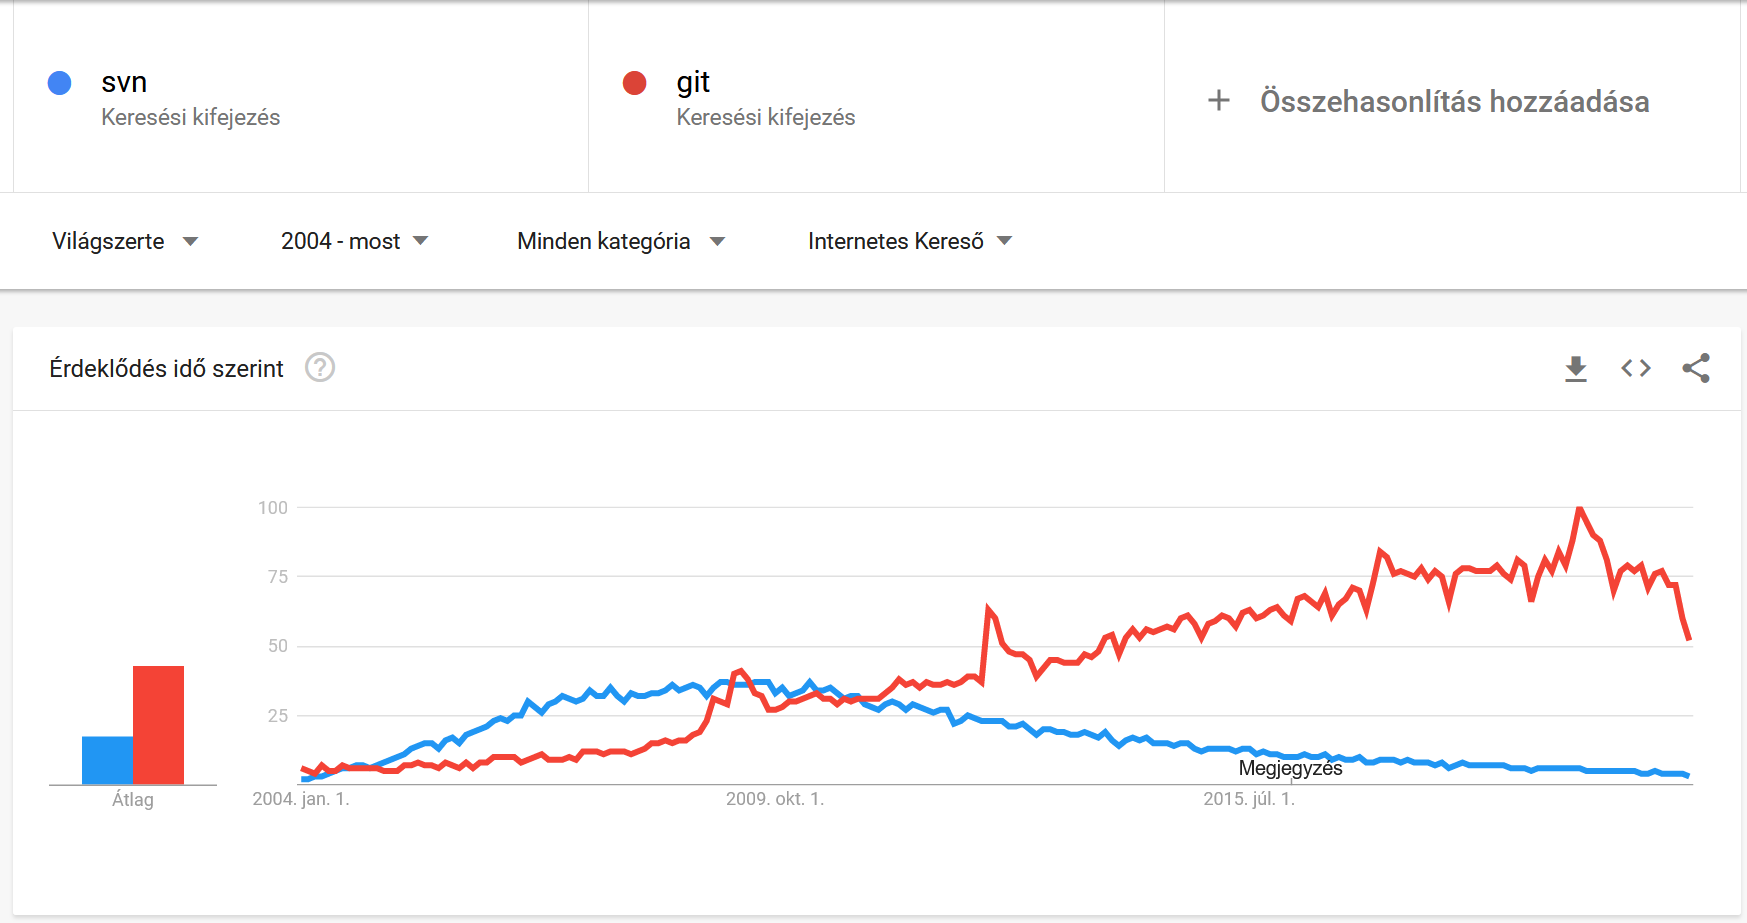
\includegraphics[width=0.8\textwidth]{images/gitsvn.png}
    \caption{A git és SVN népszerűségének változása Google Trends szerint 2004 és 2020 között}
    \label{fig:git-svn-trends}
\end{figure}


Manapság a git a de factor verziókezelő rendszer mind ipari, mind nyílt forráskódú környezetekben, amitől csak nagyon specializált esetekben szokás eltérni -- ilyenek például az egyes tech óriások monorepository-jai, amik a cég teljes forráskódját hivatottak tárolni (ezek a cégek általában saját fejlesztésű verziókezelőt használnak), vagy az olyan projektek, ahol binárisok is verziókövetve vannak (a git teljesítményét már viszonylag kis mennyiségű követett bináris is nagyon érzékenyen érinti).

Korábban már tisztáztunk pár alapvető koncepciót a verziókezelőkkel kapcsolatban, azonban a git megértéséhez pár másikról is szót kell ejteni.

\begin{itemize}
    \item \textit{Decentralized Version Control}: decentralizált verziókezelő alatt azt kell érteni, hogy minden fejlesztő gépén egy teljes értékű repository található, ami képes teljesen önálló működésre központi szerver nélkül. Ez szöges ellentéte például a Perforce-nak, ahol a depo és a fejlesztő gépén lévő repository között gyakorlatilag folyamatos interakcióra van szükség
    \item \textit{Working copy}: egy git repository másolata
    \item \textit{Staging area}: a working copy-n végrehajtott változtatásokat a staging area-ba kell mozgatni, mielőtt azok egy commit-ba kerülhetnek, tehát egy
    \item \textit{Remote}: egy, a lokálistól különböző git repository, aminek a branch-eivel a push és pull műveletekkel tudunk interakcióba lépni. Fontos, hogy egy remote koncepcionálisan nem egy központi repository-t jelent, még akkor sem, ha gyakorlatban az szokott lenni -- egy remote lehet akár csak egy lokálisan tárolt másik másolata a repository-nak, a lényeg, hogy git repository legyen
    \item \textit{Push}: "toljuk fel" a lokális history-t a push-nak megadott távoli branch felé
    \item \textit{Pull}: a push-al ellentétes művelet. Húzzunk le a remote egy adott branch-éről az ott lévő history-t a working copy-ba.
\end{itemize}

\subsection{Code smell-ek nyomai a verziókezelőkben}

Itt az ideje részleteiben kitérni a \textit{Software Design X-Rays}\cite{tornhillXrays} kapcsán már említett git statisztikákra. Ugyan korábban és a későbbiekben is git statisztikaként hivatkozom az itt prezentált statisztikákra, azt fontos itt megjegyezni, hogy ezek tökéletesen alkalmazhatóak akármelyik másik verziókezelő szoftverre is, ami érti valamilyen formában a commit, history és author koncepciókat. A git azonban, ahogy a \ref{section:version_control} fejezet taglalta, messze a legnépszerűbb veriókezelő rendszer 2020-ban, ezért már csak statisztikai alapon is erre esik a választás.

\textit{Khohm et al.}\cite{khomh} kutatása négy ipari projekt vizsgálatán keresztül demonstrálta, hogy az olyan osztályok, amik code smell-eket mutatnak, azok az életciklusuk során lényegesen több változtatást vonzanak magukhoz, mint a nem-problémás fájlok.

Továbbá \textit{M. Tufano et al.} "When and Why Your Code Starts to Smell Bad"\cite{codeSmells} című kutatása azt vizsgálta, hogy a code smell-ek mikor és hogyan kerülnek be egy kódbázisba. A konklúzió a következő lett:
\begin{enumerate}
    \item Az esetek jelentős többségében a code smell-ek az osztályok születésétől jelen vannak, ellentétebn a közhiedelemmel, miszerint a kód evolúciójának a következményei
    \item A code smell-től szenvedő osztályok és fájlok más fejlődési trendeket mutatnak, mint a "tiszta" társaik
    \item A code smell-ek jellemzően új feature-ök fejlesztése közben kerülnek be a kódbázisba, azonban a mintában nem inszignifikáns mennyiségű code smell került be refactor-t tartalmazó commit-okban
    \item A code smell-ek bevezetése általában olyan fejlesztőkhöz köthetőek, akik magas terhelés alatt vannak
\end{enumerate}

Ezekből a tanulságokból kifejezetten a 2-es pontot fogjuk megvizsgálni a \ref{ch:results} fejezetben.

\section{Tesztelés}

A modern szoftverfejlesztés egyik legnagyobb előrelépése az volt, hogy sikerült már az átlag fejlesztő fejébe is beültetni azt az egyszerű gondolatot, hogy az automatizált tesztelés minden projekten kritikus. Továbbá azt is egyre többen kezdik megérteni, hogy a teszt kód ugyanannyira fontos, mint az éles kód: a tesztek egyfajta kettős könyvelésként működnek a szoftverfejlesztés világában.

\begin{figure}[H]
    \centering
    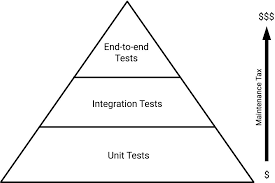
\includegraphics[width=0.8\textwidth]{images/piramis.png}
    \caption{Tesztelési piramis}
    \label{fig:testing-pyramid}
\end{figure}

\subsection{Magasabb szintű tesztek}

A tesztelési piramis legfelsőbb szintjén találjuk az E2E, azaz end-to-end teszteket. E2E teszt alatt, ahogy a neve is mutatja egy olyan tesztet értünk, ami a teljes szoftvert teszteli, jellemzően vagy egy UI-ról vagy egy REST endpoint-ról elindulva. Az automatizált UI tesztek egy specializált, nagyon gyakran alkalmazott variánsát képezik az E2E teszteknek -- ezekkel azt lehet elérni, hogy a szoftver belső működésének ismerete nélkül teszteljük úgy a teljes szoftvert, mintha a felhasználók kezében lenne.
A webes világban például a Selenium, WebDriver és Cypress segítségével leírhatjuk, hogy a tesztek milyen elemeket keressenek egy weboldalon, milyen interakciókat végezzenek ezeken az elemeken, illetve minek kell történnie az interakciók hatására.

Közvetlenül az E2E tesztek alatt helyezkednek el az integrációs tesztek. Az integrációs tesztek abból a szempontból hasonlítanak az E2E tesztekre, hogy a céljuk valamilyen szinten éles körülmények között tesztelni a kódbázis több rétegét. Az éles körülmények alatt jellemzően azt kell érteni, hogy a kód és egy külső erőforrás integrációját tesztelik.
Például képzeljük el azt, hogy szeretnénk ellenőrizni, hogy a web service-ünk a megfelelő sorokat szúrja be a vele kapcsolatban álló adatbázissal. Ezt egy unit tesztben úgy ellenőriznénk, hogy az adatbázis absztrakció megfelelő függvényét ellenőriznénk, hogy meg lett-e hívva. Egy integrációs teszt esetében ugyanezt úgy ellenőrizzük, hogy magán az adatbázison nézzük meg, hogy az adott sor bekerült-e.

\begin{figure}[H]
    \centering
    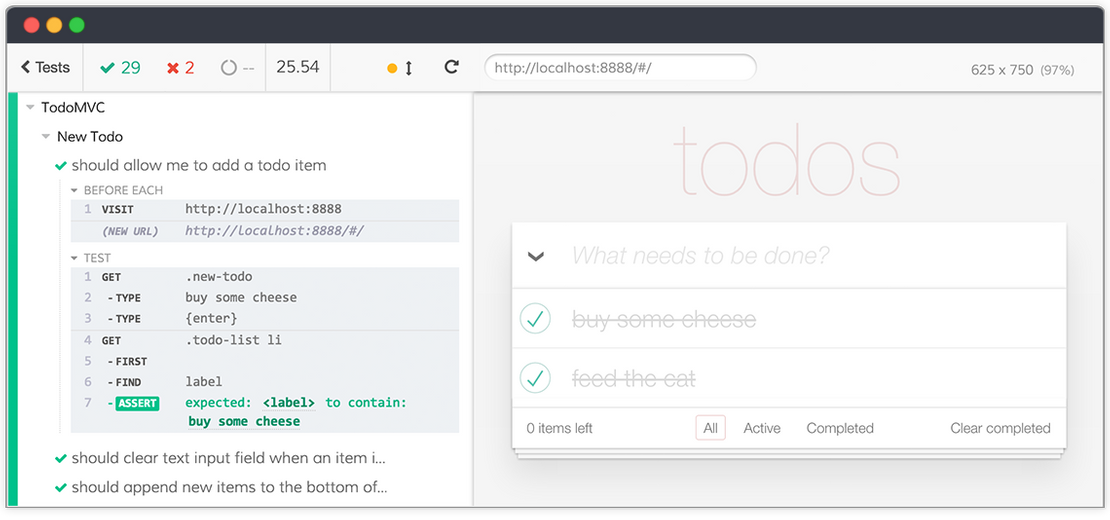
\includegraphics[width=1\textwidth]{images/cypress.png}
    \caption{Egy Cypress-ben futtatott E2E teszt}
    \label{fig:cypress-example}
\end{figure}

\subsection{Unit tesztelés}

A tesztelési piramis legalsó szintjén található a unit tesztelés. \textit{Unit teszt} alatt egy olyan tesztet értünk, ami izolációban teszteli egy nagyon specifikus részét a kódnak. Izoláció alatt itt azt értjük, hogy a tesztelt egység függőségei mock-olva vannak, azaz teszt objektumokra vannak cserélve.

A pontos definíció ebben az esetben erősen vitatott, mert gyakorlatban a unit tesztelésnek több különböző stílusa létezik. Jellemzően ezek a stílusok eltérnek az izoláció mértékében, a tesztelt kód specificitásában és az ellenőrzések formájában is. Sok projekt továbbá kombinálja ezeket a különböző stílusokat az alkalmazás különböző rétegeiben.

Definíciótól függetlenül azonban a unit tesztek célja világos: bizonyítsuk, hogy a kód, amit írtunk tényleg úgy viselkedik, ahogy szeretnénk és ez a verifikáció legyen könnyen és gyorsan megismételhető.

Ellentétben a korábban már említett integrációs és E2E tesztekkel, a unit tesztek fehér doboz tesztek, ami azt jelenti, hogy a teszt maga részleteiben ismeri a tesztelt kódot, hiszen direkt interakcióban van vele.

\begin{figure}[H]
    \centering
    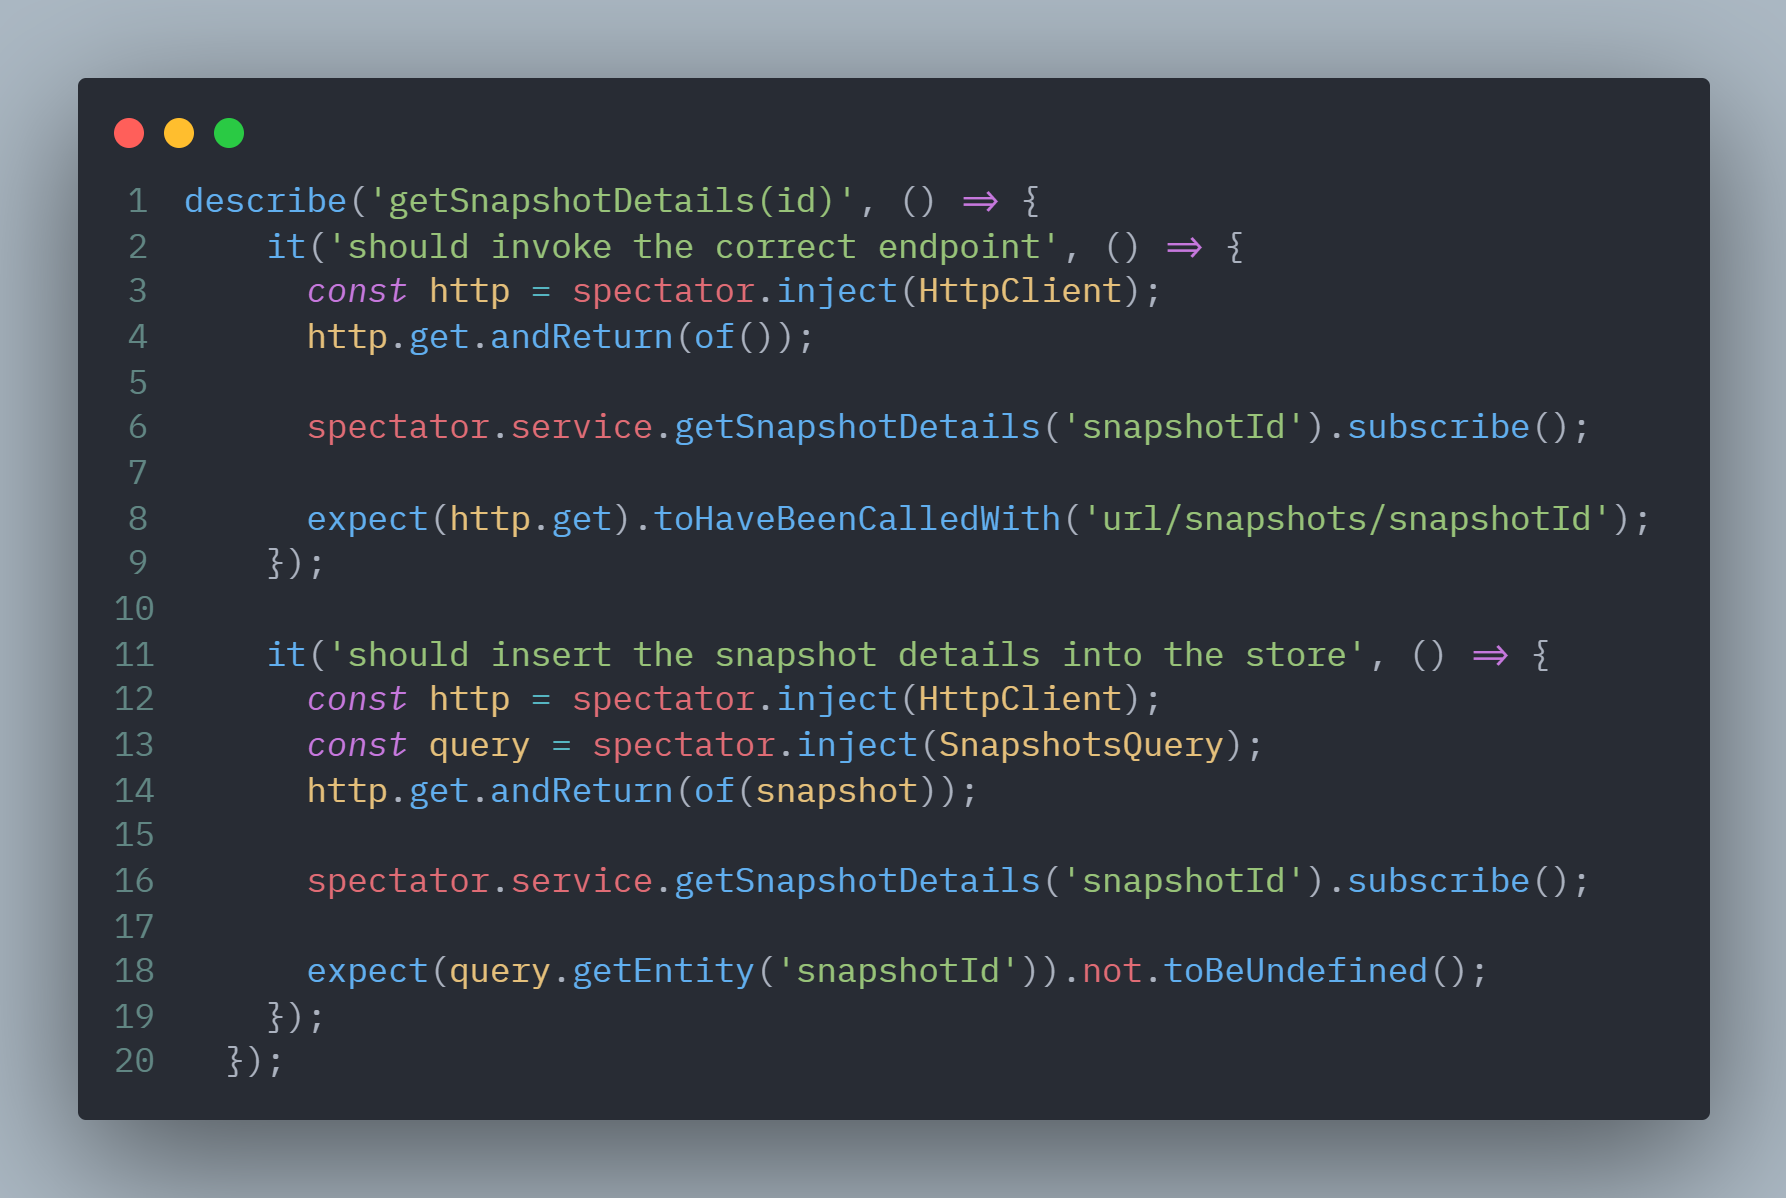
\includegraphics[width=0.8\textwidth]{images/unit-test.png}
    \caption{Unit teszt a Hestia UI projektből}
    \label{fig:unit-test-example}
\end{figure}

\begin{figure}[H]
    \centering
    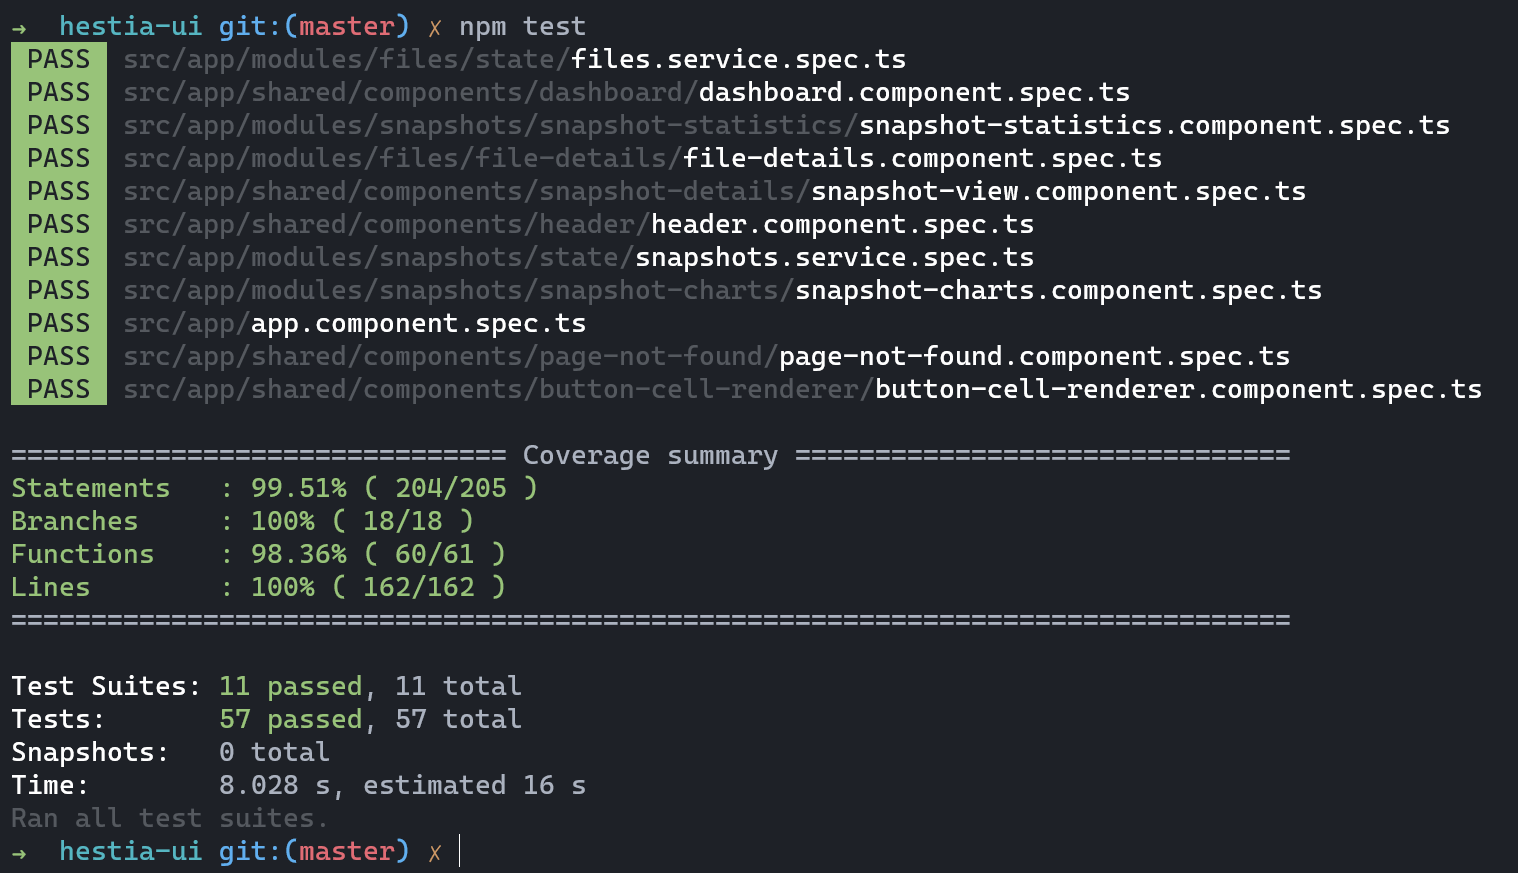
\includegraphics[width=0.8\textwidth]{images/testRun.png}
    \caption{Unit tesztek futtatása}
    \label{fig:unit-test-run-example}
\end{figure}

\section{Teszt coverage}

Tisztáztuk a korábbiakban a tesztelés alapvető célját és a különböző szintjeit, azonban arról még nem esett szó, hogy milyen metrikákat tudunk kinyerni egy kódbázis tesztjeiből. Itt jön képbe a teszt coverage, ami azt mutatja, hogy a futattott tesztek milyen arányban hajtják meg az éles kódot, bizonyos szempontok szerint. Jellemzően a következő különböző szinten értelmezzük a coverage-et:
\begin{itemize}
    \item \textit{Statement coverage}: todo
    \item \textit{Line coverage}: todo
    \item \textit{Function coverage}: a kódbázisban lévő függvények
    \item \textit{Branch coverage}: vezérlési struktúrák ágainak coverage értéke
    \item \textit{Condition coverage}: boolean
\end{itemize}

\begin{figure}[H]
    \centering
    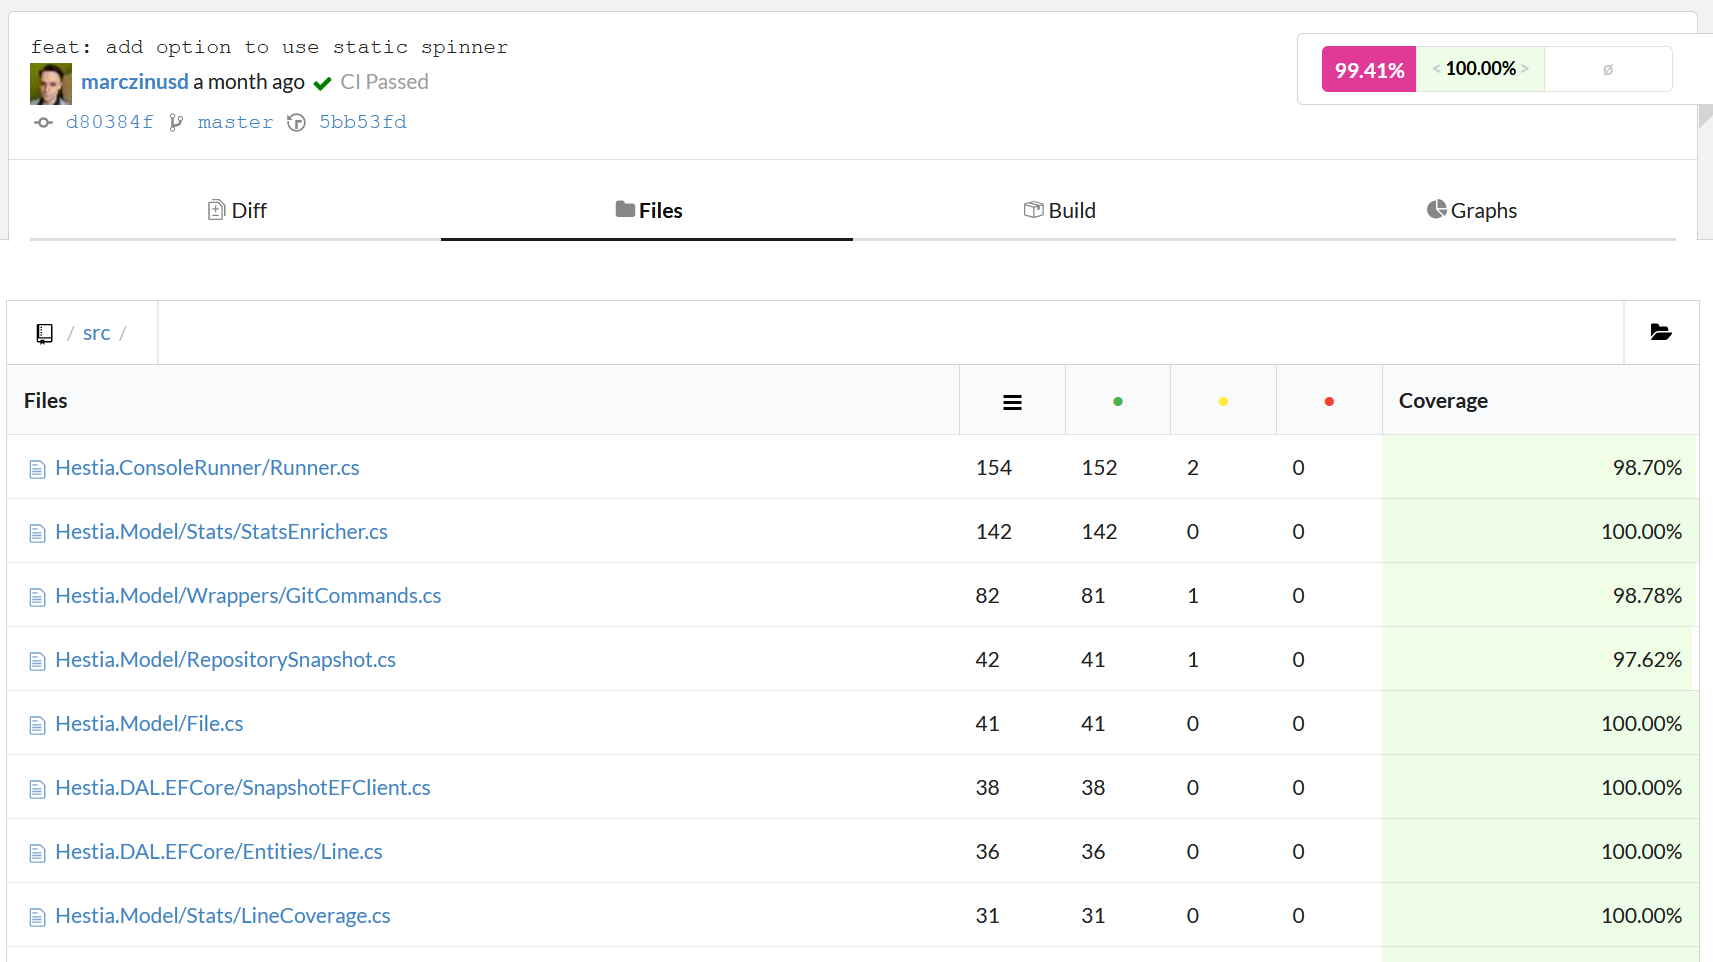
\includegraphics[width=1\textwidth]{images/codecov-report.png}
    \caption{Egy coverage report a codecov.io oldalról}
    \label{fig:codecov-example}
\end{figure}

Technikailag a tesztelési piramis minden szintjéből generálható coverage report, de ahogy haladunk felfelé a hierarchiában, ez egyre nehezebb és kevésbé releváns lesz.

\subsection{Kódminőség és a teszt coverage}

A coverage gyakran kerül említésre, mint egy mérce, ami valamilyen mértékben reprezentálja a kódminőséget. Felmerülhet azonban a kérdés, hogy a code coverage valóban mércéje-e a kódminőségnek. Több kutatás \cite{onRelation}\cite{singhkochhar:hal-01653728} vizsgálta azt, hogy milyen kapcsolatban áll a code coverage és a kódminőség, ahol a kódminőség alatt a szoftverhibák alacsony számát értjük. Ezek a kutatások azt mutatják, hogy a korreláció a coverage és a minőség között alacsony. A "Mythical Unit Test Coverage"\cite{mythical} tovább viszi ezt az ötletet és a code coverage-et a változtatások komplexitásával párosítja, hasonló eredménnyel, mint a korábbi kutatások: a code coverage önmagában nem elégséges metrika a kódminőség meghatározására.

Az előbbiekből könnyen levonhatnánk konklúzióként, hogy a coverage kódminőségi metrikaként való használata legjobb esetben is spekulatív, hiszen több kutatás mutat abba az irányba, hogy a korreláció a kódminőség és a coverage között valahol a nem létező korreláció és a gyenge korreláció között van, amennyiben a kódminőséget abban mérjük, hogy mennyi hiba képes bekerülni egy éles szoftverbe.

Reálisan nézve viszont sem a kódminőség, sem maga a szoftverfejlesztés nem ennyire egzakt. Akárki, aki dolgozott legacy projekten tisztában van azzal, hogy mekkora a különbség egy olyan kódbázis között, ahol a legkisebb refactor-t is lehetetlen automatizáltan tesztelni és egy olyan között, ahol minden osztályt fed legalább egy pár viszonylag triviális teszt. Nyilvánvaló, hogy a code coverage önmagában egy gyenge metrika, azonban egyéni, fejlesztői szempontból a különbség egy 50\%-os és egy 98\%-os code coverage-el rendelkező projekt között távolról sem marginális.

A unit tesztelés és így a coverage hatása a sokkal kevésbé mérhető fejlesztői kultúrában manifesztálódik és csatlakozik ebben az aspektusában a statikus kódelemző eszközökhöz, mint a SonarQube\footnote{https://www.sonarqube.org/}, vagy a webes világból ismert linter-ek\footnote{https://eslint.org/}. Mind a unit tesztelés, mind a statikus kódelemzésnek a gyakorlati hatása a már korábban említett code smell-ek moderációjában mérhető. Ha egy fejlesztő csapat kötelezővé tesz egy bizonyos coverage értéket a kódbázison, akkor ez valamilyen formában önreflekcióra kényszeríti a fejlesztőket a tesztek írása közben, ami továbbá erősíti a fejlesztőkben a minőség-orientált kultúrát.

Vegyük példának a \textit{God Object} code smell-t. Az ilyen osztályokat egy idő után nagyon nehéz tesztelni, mert egyrészt a külső függőségek száma az osztály méretével együtt nő, másrészt pedig az osztály belső állapota és komplexitása is folyamatosan nőni fog, amit egyre nehezebb tesztekben lekövetni. Ha van egy coverage gating a projekten és a fejlesztői kultúra része, hogy minőségi teszteket kell produkálni minden új funkcionalitáshoz, akkor a \textit{God Object} esetében két dolog történhet:

\begin{enumerate}
    \item Az osztály egyre tovább nő, egyre nehezebb teszteket írni az új funkcionalitásra, ami először frusztrációhoz, majd pedig jobb esetben reflekcióhoz vezet
    \item A fejlesztők felismerik az osztály problémáit és a meglévő teszteket felhasználva elkezdik szétbontani kisebb darabokra
\end{enumerate}

Az 1-es lehetőség eredménye általában az, hogy a fejlesztők elkezdik megkerülni a \textit{God Object}-et ahol csak lehet. Ez nem feltétlen ideális, de a frusztráció és indirekt reflekció az osztály működése miatt moderáló hatással lesz az osztály további növekedésére nézve ahhoz az esethez képest, ahol ugyanez az osztály mentes minden teszttől és duzzadhat tovább mindenféle kontroll nélkül.

A 2-es az ideális eset. Ha maga az osztály kódja nem is, de a tesztek segítettek egyrészt felismerni a problémát, másrészt pedig elősegítették az osztály lebontását, ami hosszú távon egészségesebb kódhoz vezet.

Ahelyett tehát, hogy minőségi metrikaként tekintünk a coverage-re, érdemesebb úgy gondolni rá, mint a kód karbantarthatóságának az egyik metrikája.

\section{A teszt coverage és git statisztikák közös vizsgálata}

Most, hogy körbejártuk mind a git statisztikákat, mind a tesztelési kérdéseket és metrikákat, itt az ideje arról is szót ejteni, hogy pontosan mit fog ez a diplomamunka vizsgálni és mi a feltételezés.

Azt könnyű belátni, hogy mind a git statisztikák, mind a code coverage hasonló koncepciókkal dolgoznak (fájl- és sorszintű, könnyen mérhető és szemrevételezhető heurisztikák), így kézenfekvő ötletnek tűnik a kettő együttes vizsgálata. A vizsgálat célja, hogy egyrészt maguknak a git statisztikáknak az evolúcióját próbáljuk értelmezni a kódbázisok élettartama alatt és ebből vonjunk le következtetéseket. A másodlagos cél az az, hogy nézzük meg milyen kapcsolatban áll a git statisztikák alakulása a teszt coverage-el. Van-e moderáló hatása a teszt coverage-nek a gyakran változtatott fájlokon? Hogy alakul a coverage ezeken a fájlokon -- konstans marad, romlik, vagy esetleg nő?


\cleardoublepage

\chapter{A programról}
\label{ch:about_hestia}

\section{Motiváció}

Felmerülhet a kérdés, hogy pontosan miért van szükség jelen esetben egy új programra -- git-ből kinyerhetőek a vizsgálathoz szükséges statisztikák akár csak egy egyszerű bash script segítségével, a coverage adatokat pedig a már amúgy is generált report-ból szemre meg tudjuk vizsgálni.

Egyrészt a triviális és sok szoftverfejlesztési projekt motivációjaként szolgáló válasz itt is a kényelem és automatizálás. Természetesen lehet bash script-eket használni, kézzel feldolgozni a kimenetüket, majd szemmel összenézni azt egy tetszőleges formátumú coverage report-al, de ez nem éppen ideális felhasználása egy fejlesztő idejének, főleg nem akkor, ha ezt sokszor meg kell ismételni.

Másrészt fontos megjegyezni, hogy ugyan specifikusan a vizsgálat számára releváns git statisztikák követésére léteznek megoldások (nevezetesen például a korábban már említett \citeauthor{tornhillXrays} által fejlesztett, fizetős CodeScene\footnote{CodeScene: https://codescene.io/}, illetve az annál sokkal egyszerűbb GitNStats\footnote{GitNStats: https://github.com/rubberduck203/GitNStats}), ezen megoldások azonban nem használják ki a coverage által nyújtott extra lehetőségeket.

\section{Architektúra}

A program, ami a Hestia becenevet kapta, két nagy részből áll:
\begin{enumerate}
    \item Hestia: a teljes modellt ábrázoló, perzisztáló és a kliens felé kiszolgáló .NET 5 alapokon írt program
    \item Hestia-UI\footnote{Forráskód: https://github.com/marczinusd/hestia-ui}: Angular 11-ben írt vékony kliens ami REST API-n keresztül kéri le a .NET-es web service-től az adatbázisba mentett repository-kat
\end{enumerate}

\section{A modell}

Mielőtt részletesen ismeretetném a programokat, előbb fontos tisztázni a koncepciókat és terminológiákat, amikre a projekt mindkét rétege épít. A bevezetésben elhangzott egy rövid bevezetés a git verziókövetőbe és a unit teszt coverage-be, illetve említésre került, hogy a jelen végzett analízis szempontjából nagyon hasonló absztrakciókkal dolgozik mindkettő.

A modell legmagasabb szintű absztrakciója maga a repository: ez értelemszerűen egy projekt teljes forráskódjának a git-ben való leképezése.

Közvetlen a repository-hoz alatt lévő absztrakció az úgynevezett snapshot. Ezalatt egy repository egy adott commit-jánál megfigyelt állapotot értjük. Maga a git nem értelmezi pontosan ezt a koncepciót, illetve a coverage report-ok szempontjából is ekvivalens gyakorlatban egy snapshot és egy repository, mégis érdemes tisztázni, hogy pontosan mit jelent, mert a későbbiekben fontos lesz, hogy egy repository állapotát több, hozzá tartozó snapshot-on keresztül figyeljük meg.

A snapshot-okhoz közvetlen kapcsolódik fájlok egy halmaza. Ez az első réteg, amit mind a git, mind egy coverage report definiál. Itt fontos megjegyezni a statisztikákat, amiket a program képes kinyerni fájl-szinten:
\begin{enumerate}
    \item Egyedi szerzők száma
    \item Commit-ok száma, amik tartalmazták az adott fájlt
    \item Fájl-szintű coverage arány
\end{enumerate}

A modell legalsó rétegét egy fájlban található forráskód sorai képezik. Egy sorhoz a program a következő statisztikákat társítja:
\begin{enumerate}
    \item Egyedi szerzők száma
    \item Commit-ok száma, amik értintették az adott sort
    \item Unit tesztek száma, amik értintették az adott sort
    \item Branch coverage
\end{enumerate}

A gyakorlatban a sorok statisztikái kiemelkedően hasznosak, hiszen betektintést adnak egy fájl kiemelkedően problémás részeire, ajánlást adva potenciális refactor-ra. Ebben a diplomamunkában végzett analízis szempontjából azonban a fájl-szintű statisztikák lesznek relevánsak, mivel mintákat próbálunk keresni teljesen ismeretlen kódbázisokban.

\section{Hestia - a backend modell}

Az előző szekcióban ismertetett modellt, illetve logikát implementálja a Hestia. A program .NET 5-ben készült, ami azt jelenti, hogy teljesen platformfüggetlen: tesztelve lett Windows 10, Linux és MacOS operációs rendszerek alatt. Itt fontos azonban megjegyezni, hogy bár a platformfüggetlenség garantált, a git természetéből fakadóan abszolút nem mindegy, hogy milyen operációs rendszeren futtatjuk a repository analíziseket, hiszen a git notóriusan lassú a Windows fájlrendszerein -- nagyságrendileg tízszer tovább fog tartani egy Windows-on futtatott analízis a Linux-on vagy MacOS-en futtatott analízissel szemben.

Maga a program stílusát tekintve funkcionális koncepciókra épít: kap egy bemeneti értékhalmazt és azokat tiszta függvényeken keresztül transzformálja addig, amíg egy coverage és git statisztikákkal rendekező snapshot-ot nem kapunk. Itt emelném ki a nagyszerű language-ext\footnote{language-ext: https://github.com/louthy/language-ext} nevű könyvtárat, ami a C\# funkcionális repertoárját egészíti ki, ezzel elősegítve a Hestia modelljének funkcionális tisztaságát.

A felépített modellt a program Entity Framework Core segítségével tetszőleges adatbázisban képes tárolni az eredményeket -- per pillanat SQLite-ra van konfigurálva a projekt a könnyű hordozhatóság és tesztelhetőség érdekében, de ez triviális mennyiségű munkával átírható a népszerűbb adatbázisok akármelyikére.

\section{Konzolos futtató}

A repository analízisek gyors, könnyen ismételhető futtatása kritikus követelménye volt a projektnek. Eleinte egy grafikus futtató felülettel kísérleteztem, de hamar kiderültek a hátrányai (nevezetesen az ismételhetőség volt problémás), így a konzolos futtatás maradt az egyetlen opció. Egy repository-ra mindössze egy relatíve egyszerű konfigurációs fájlt kell létrehozni az alábbi formátumban, amit a futtató végre tud hajtani:

\lstset{caption={A React projekt Hestia konfigurációja}, language=json, numberstyle=\small}
\begin{lstlisting}
{
  "$schema": "https://raw.githubusercontent.com/marczinusd/hestia/master/src/Hestia.ConsoleRunner/config.schema.json",
  "coverageReportLocation": "~/dev/react/coverage/lcov.info",
  "repoRoot": "~/dev/react",
  "sourceRelativePath": "packages",
  "fileExtensions": [".js", ".ts"],
  "statGranularity": "full",
  "ignorePatterns": [],
  "buildCommands": ["yarn install"],
  "testCommands": ["yarn test --coverage"]
}
\end{lstlisting}

Műveletigény szempontjából a konfigurációs fájl tartalmaz egy nagyon fontos paramétert \code{statGranularity}, ami lehet "full", vagy "file". Amennyiben file értéket kap, akkor csak fájl-szintű git statisztikákat generálunk, aminek a műveletigénye (élve azzal a feltételezéssel, hogy a git parancsok műveletigényét konstansnak tekintjük) \( \theta(n) \), ahol \(n\) alatt a repository-ban lévő fájlok számát értjük. Ha full-ra állítjuk ezt az opciót, akkor egy analízis műveletigénye \( \theta(n + m) \), ahol \(n\) a fájlok száma, \(m\) alatt pedig a repository-ban lévő összes kódsorok számát értjük. Ráadásképp könnyű azt is belátni, hogy \(m\) nagyságrendekkel nagyobb lesz \(n\)-nél, tehát a végső műveletigény \( \theta(m) \). Ez azt jelenti, hogy egy fájl-szintű vizsgálat futási ideje még egy nagy repository esetében is a másodperces nagyságrendben lesz, a sor-szintű analízis ezzel szemben viszont egy kis repository esetében is percekig fut.

Gyakorlatban egy konzolos futtatást a következő módon néz ki:
\begin{enumerate}
    \item Ha volt megadva a konfigurációs fájlban build lépés sorozat, akkor futtassuk le őket
    \item Ha volt megadva a konfigurációs fájlban teszt lépés sorozat, akkor futtassuk le őket
    \item Szűrjük ki a létrehozott snapshot-ból azon fájlokat, amik nem felelnek meg a konfigurációban megadott szűrőknek
    \item Konvertáljuk át a megadott coverage report-ot cobertura formátumra
    \item Adjuk hozzá a létrehozott snapshot-hoz a git statisztikákat
    \item Adjuk hozzá a létrehozott snapshot-hoz a coverage statisztikákat
    \item Mentsük el adatbázisba a snapshot végleges formátumát
\end{enumerate}

\begin{figure}[H]
    \centering
    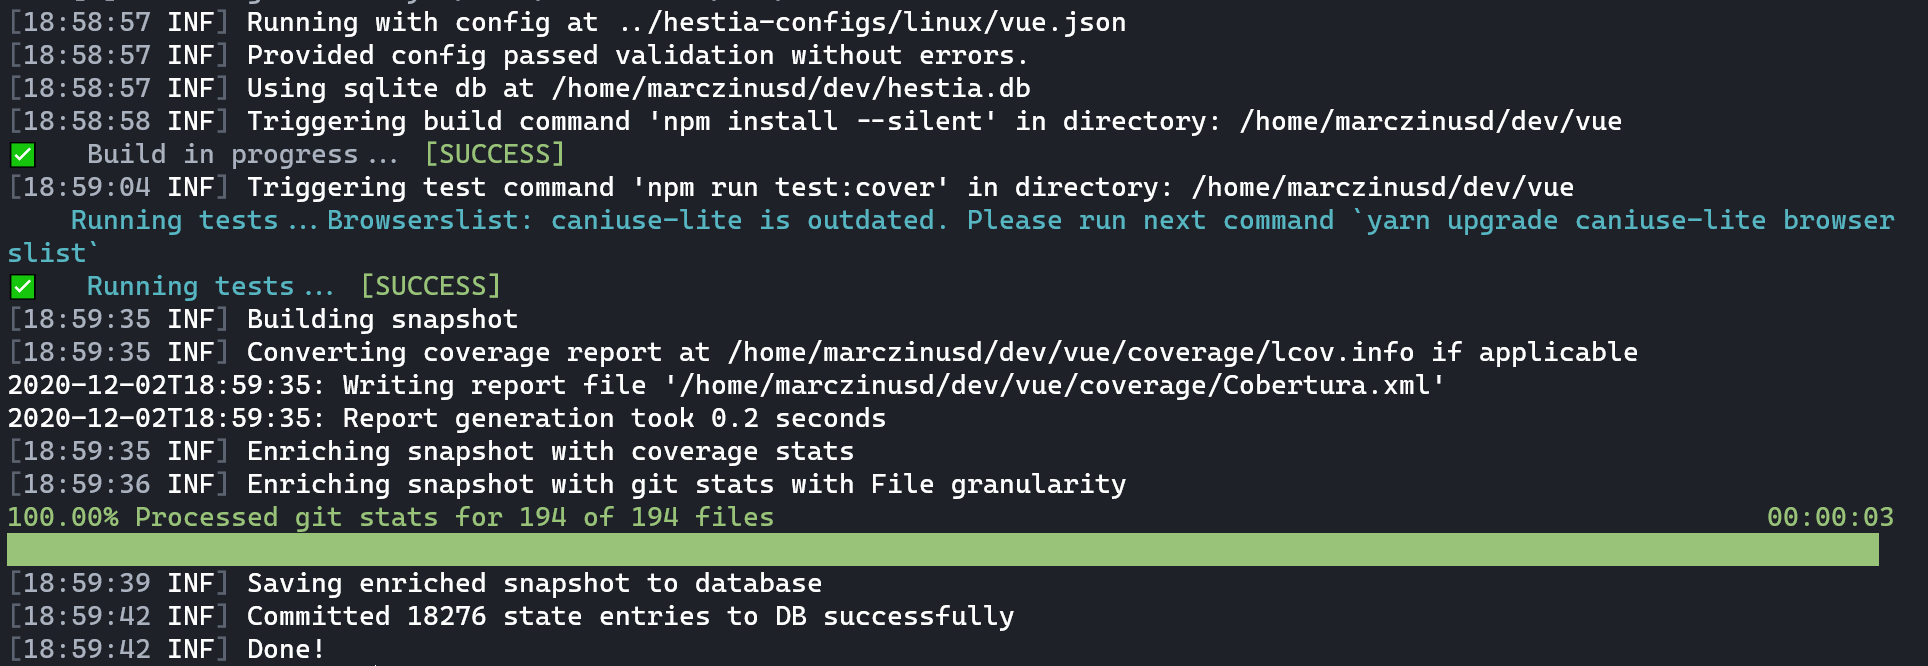
\includegraphics[width=1\textwidth]{images/hestia-console-run-vue.png}
    \caption{A konzolos futtató működés közben}
    \label{fig:console-runner-example}
\end{figure}

Fontos megjegyezni, hogy bár a konzolos futtató per pillanat csak egyedi snapshot analízis futtatásra lett felkészítve, maga a háttérben lévő modell képes repository-szintű analízisre is.

A repository-szintű analízis annyiban más, hogy paraméterül kap egy számot, ami a mintavételezési sűrűséget reprezentálja, azaz azt, hogy egy repository-ból hány snapshot-ot szeretnénk készíteni. Ugyan ez a fajta analízis is hasznos, a probléma jelenleg abban rejlik, hogy egy repository commit-jai nem egyenletesen oszlanak el az időben, így az implementáció, ami egyenletesen veszi a mintákat a commit-ok számának tekintetében, torzítani fogja az ereményeket a manuális mintavételezéssel szemben, ahol szempontnak számítanak többek között a szoftverfejleszétis mérföldkövet is.

\section{Web service}

A Hestia backend-jének utolsó nagy részét a ASP.NET Web API alapú, REST-es web service képezi. Ez tulajdonképpen arra hivatott, hogy a konzolos futtatás eredményeit szolgálja ki a külvilág számára könnyen emészthető módon, json formátumban. A service a következő endpoint-okat definiálja:
\begin{itemize}
    \item GET /snapshots: adjuk vissza az összes elérhető snapshot-ot, a snapshot teljes részletei nélkül
    \item GET /snapshots/\#snapshotId: adjuk vissza a megadott ID-hez tartozó snapshot részleteit
    \item GET /files/\#fileId: adjuk vissza a megadott ID-hez tartozó fájl részleteit
\end{itemize}

A service továbbá host-ol egy Swagger UI-t, ami dokumentálja és kipróbálhatóvá teszi az összes endpoint-ot. A service elindítása után a Swagger UI a \code{https://localhost:5001/index.html} címen érhető el.

\section{Hestia UI - Vékony kliens}

A webes kliens egy Angular 11-ben készült és szintén nagyban funkcionális és reaktív programozási koncepciókra épít az RXJS\footnote{https://github.com/ReactiveX/rxjs} segítségével, illetve modern state management-et implementál az Akita\footnote{https://github.com/datorama/akita} nevű könyvtár használatával. A webes kliens modellje megfelel a korábban definiált modellnek, TypeScript-ben implementálva.

A kliens képes megmutatni:
\begin{itemize}
    \item Az összes elérhető snapshot-ot
    \item A snapshot mögött lévő fájlokat a statisztikákkal párosítva, táblázatos formátumban
    \item A fájlok tartalmát sor-szintű statisztikákkal egy Monaco szövegszerkesztőben
    \item Snapshot-szintű statisztikákat grafikonokon ábrázolva
\end{itemize}

\begin{figure}[H]
    \centering
    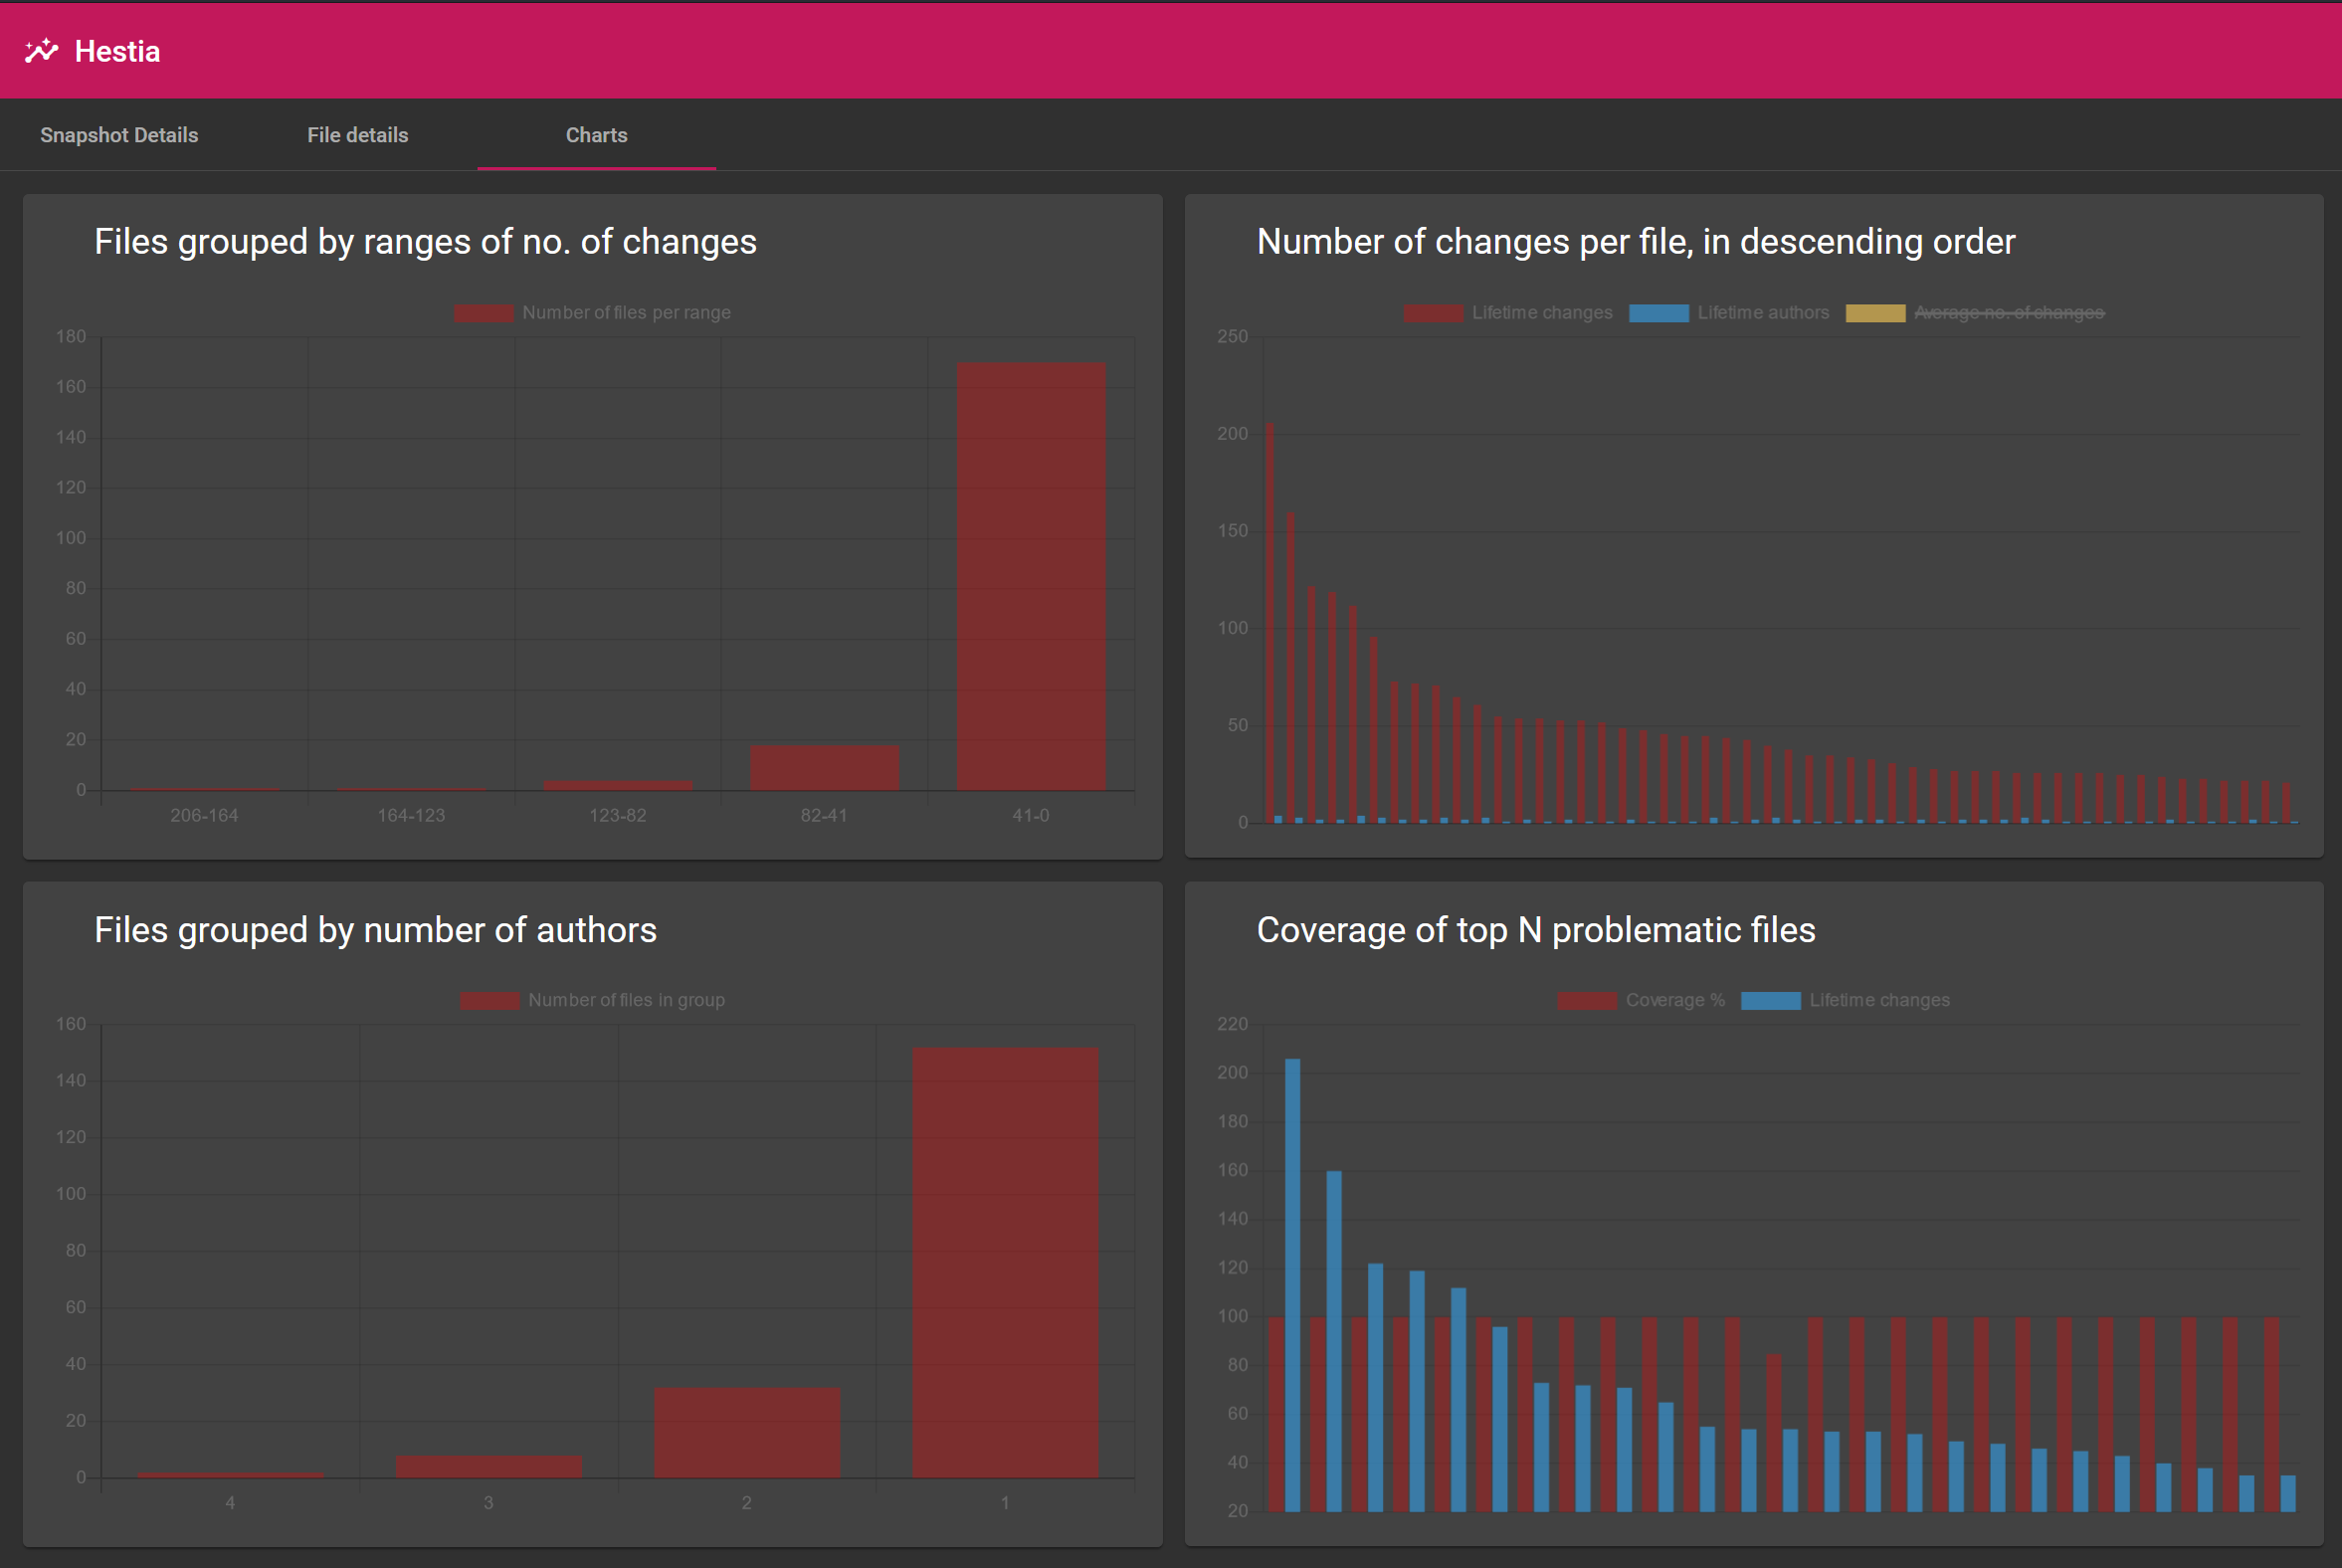
\includegraphics[width=1\textwidth]{images/hestia_charts.png}
    \caption{A vékony kliens által generált grafikonok}
    \label{fig:hestia-charts}
\end{figure}

\section{A program használata}

A .NET alapú konzolos futtató és web service használatának egyetlen előfeltétele, hogy a .NET 5 SDK\footnote{https://dotnet.microsoft.com/download/dotnet/5.0} telepítve legyen. A könnyebb futtatáshoz erősen ajánlott továbbá a GNU Make\footnote{https://www.gnu.org/software/make/} is, mert azzal elérhetővé válnak a dedikált build target-ek, amiket a továbbiakban részletezni fogok. Amennyiben a make nem áll rendelkezésre, akkor a projekt gyökerébem lévő makefile megfelelő build target-jének a parancsait kell sorrendben futtatni.

Első lépésben a forráskódot\footnote{https://github.com/marczinusd/hestia} git segítségével le kell tölteni, majd a projekt gyökerében állva a következő módon tudjuk futtatni a programot:

\begin{itemize}
    \item Analízis futtatása konzolon keresztül: \code{make run-console -{}- -{}-configPath "/path/to/config-file.json" }, ahol a konfigurációs fájl a korábban megadott formátumban van
    \item Web service indítása: \code{make run-webservice}
\end{itemize}

A webes kliens futtatásához egyedül egy telepített NodeJS-re van szükség. A forráskód\footnote{https://github.com/marczinusd/hestia-ui} letöltése után a projekt gyökerében állva ki kell adni az \code{npm install} parancsot, majd miután az lefutott az \code{npm start} fogja kiszolgálni a webes klienst a konzolon kiírt URL-en keresztül.

\cleardoublepage

\chapter{Eredmények}
\label{ch:results}

\section{Vizsgált kódbázisok}

Egy kódbázisnak a következő feltételeket kell teljesíteni, hogy vizsgálni tudjuk:
\begin{enumerate}
    \item Legyen könnyen build-elhető, évekre visszamenően
    \item A tesztek legyenek könnyen futtathatóak
    \item Generálódjon coverage report a teszt futtatásokhoz és a report formátuma legyen egyike azoknak, amiket támogat a ReportGenerator\footnote{https://github.com/danielpalme/ReportGenerator} nevű .NET-es könyvtár
    \item A projekt legyen nyílt forráskódú
    \item Rendelkezzen a projekt viszonylag gazdag commit történettel -- jelen esetben az 5000+ commit és 3+ éves történet heurisztikát alkalmaztam
\end{enumerate}

Ezeket a feltételeket ugyan könnyű teljesíteni egy fejlesztő csapatnak ipari környezetben saját projektekre, sajnos nyílt forráskódú környezetben más a helyzet -- specifikusan az 1-es és 3-as pontok jelentenek problémát. A C++-ra, Python-ra és .NET Framework-re épülő projektek például egy az egyben kiesnek, mert egyik sem ad egyszerű módot arra, hogy a build-eléshez szükséges környezetet könnyen elő tudjuk állítani a projekt életciklusának akármely pontján.

Gyakorlatban a JavaScript NodeJS/NPM, .NET Core/.NET 5+ és Java ökoszisztémákra épülő projektek felelhetnek meg a korábbi feltételeknek. Ezek közül azonban a Java a szakmai hátterem miatt kiesik, a .NET Core/5+ projektek jelentős többsége pedig az 5-ös feltételt nem teljesíteni, így marad a JavaScript Node/NPM ökoszisztéma. A specifikus projekteknél külön meg fogom említeni, de általánosságban itt is leírom: még a JavaScript/NodeJS/NPM ökoszisztéma esetén is komoly problémát jelent a régi (~2015 előtti) verziók build-elése, mivel az NPM és a node, illetve a rájuk épített projektek sok változáson estek át az évek során, amit ma a projekt ismerete nélkül már nehéz reprodukálni. Ez azt jelenti, hogy a legtöbb esetben lehetetlen

Fontos leszögezni még egy dolgot. A JavaScript-es projektek elemzése egy jelentős vakfoltot fog képezni, méghozzá azért, mert a nyílt forráskódú projektek között gyakorlatilag lehetetlen olyat találni, amire őszintén azt lehet mondani, hogy rossz minőségű kódbázissal rendelkezik. Nyilván egy kódbázis minősége szubjektív, de a GitHub-on host-olt JavaScript projektek túlnyomó többsége 95\% feletti coverage-el rendelkezik. Ráadásul azok a projektek, amik 95\% alatt vannak, azok jellemzően csak a nagyon konzervatív coverage ignore path-ok miatt mutatnak ilyen értékeket -- a React projekt például 80\% körüli értéket mutatott, azonban hamar kiderült, hogy ez csak azért van, mert halott kódot tartanak a repository-ban, amit már nem hajtanak meg unit tesztek.

A fentieket figyelembe véve a következő projektekre esett a választás:
\begin{itemize}
    \item Vue: https://github.com/vuejs/vue
    \item Express: https://github.com/expressjs/express
    \item React: https://github.com/facebook/react
    \item Gatsby: https://github.com/gatsbyjs/gatsby
\end{itemize}

\section{Vue}

Elsőként a vue.js\footnote{\url{https://github.com/vuejs/vue}} kódbázisát fogjuk megvizsgálni. A Vue egy progresszív, JavaScript-alapú frontend framework. A Vue feature-ök tekintetében valahol a másik két nagy frontend framework, az Angular és a React között van -- nem próbál egy kikövezett utat adni, mint az Angular, de nem csak egy specifikus szeletét fedi le a frontend fejlesztésnek, mint a React.

\lstset{language=HTML, caption={Egy egyszerű Vue komponens}}
\begin{lstlisting}
<div id="app">
    {{ message }}
</div>
\end{lstlisting}

\lstset{language=JavaScript, caption={Egy egyszerű Vue komponens JS kódja}}
\begin{lstlisting}
var app = new Vue({
    el: '#app',
    data: {
        message: 'Hello Vue!'
    }
})
\end{lstlisting}

A projekt viszonylag fiatal, a fejlesztése 2016-ban kezdődött. A későbbi megfigyelések szempontjából érdemes megjegyezni, hogy ugyan jelen pillanatban 338 egyedi kontribútora van a projektnek, a fejlesztés nagy része egy fejlesztőhöz, Evan You nevéhez köthető:

\lstset{caption={A vue.js top 10 kontribútora}}
\begin{lstlisting}
vue git:(dev) git shortlog -sn | head -n10
    2303  Evan You
    78  vue-bot
    47  Hanks
    34  Eduardo San Martin Morote
    32  kazuya kawaguchi
    30  chengchao
    25  katashin
    21  AchillesJ
    18  Herrington Darkholme
    15  JK
\end{lstlisting}\label{code:vue-authors}

Az analízist a vue esetében az első publikus release-től kezdjük.

\subsection{Vue 1.0}

A vue több szempontból is különös eset lesz: egyrészt az első publikus release-ig gyakorlatilag egy egyszemélyes projekt volt, másrészt pedig, ahogy azt később látni fogjuk, a Vue 2.0 egy teljes újraírása volt a projektnek.

Először vessünk egy pillantást a \ref{table:vue1-top-files} táblázatra, amiben a vue 1.0-ás változatának legtöbbet módosított fájljai láthatóak. Látható, hogy bár egy fejlesztője van a projektnek és 100\%-os coverage-el rendelkezik, már itt kialakulóban van fájloknak egy halmaza, amik vonzani fogják magukhoz a későbbi változtatásokat és javításokat. A \code{compile.js}, \code{directive.js} és \code{watcher.js} fájlokra kiemelten érdemes figyelni, mert ezek már most kiemelkednek az átlagból méret és változtatások száma tekintetében (átlag fájl méret 147, átlag változtatások száma 20 a teljes repository-ra).

\begin{table}[h]
    \centering
    \begin{tabular}{l|l|l|l|l}
        Filename      & Lifetime Authors & Lifetime Changes & Line Count & Coverage \% \\ \hline
        compile.js    & 2                & 123              & 709        & 100         \\
        directive.js  & 1                & 102              & 320        & 100         \\
        init.js       & 1                & 80               & 114        & 100         \\
        watcher.js    & 3                & 72               & 344        & 100         \\
        vue.js        & 1                & 52               & 96         & 100         \\
        lifecycle.js  & 1                & 49               & 68         & 100         \\
        data.js       & 1                & 45               & 174        & 100         \\
        lang.js       & 4                & 44               & 388        & 100         \\
        dom.js        & 2                & 42               & 362        & 100         \\
        transclude.js & 2                & 40               & 148        & 100         \\
        global.js     & 1                & 39               & 152        & 100
    \end{tabular}
    \caption{A vue 1.0-ás kiadásának leggyakrabban módosított fájljai} \label{table:vue1-top-files}
\end{table}

Érdekes továbbá a változtatások számáról készített hisztogram a \ref{fig:vue1-hist} ábrán, amiről jól látszik, hogy a 67 forrás fájlból álló vue 1.0 változtatásainak egy jelentős része 5 fájl köré csoportosul, amik méret és változtatás szám szepontjából már most az átlag többszörösét mutatják.

\begin{figure}[h]
    \centering
    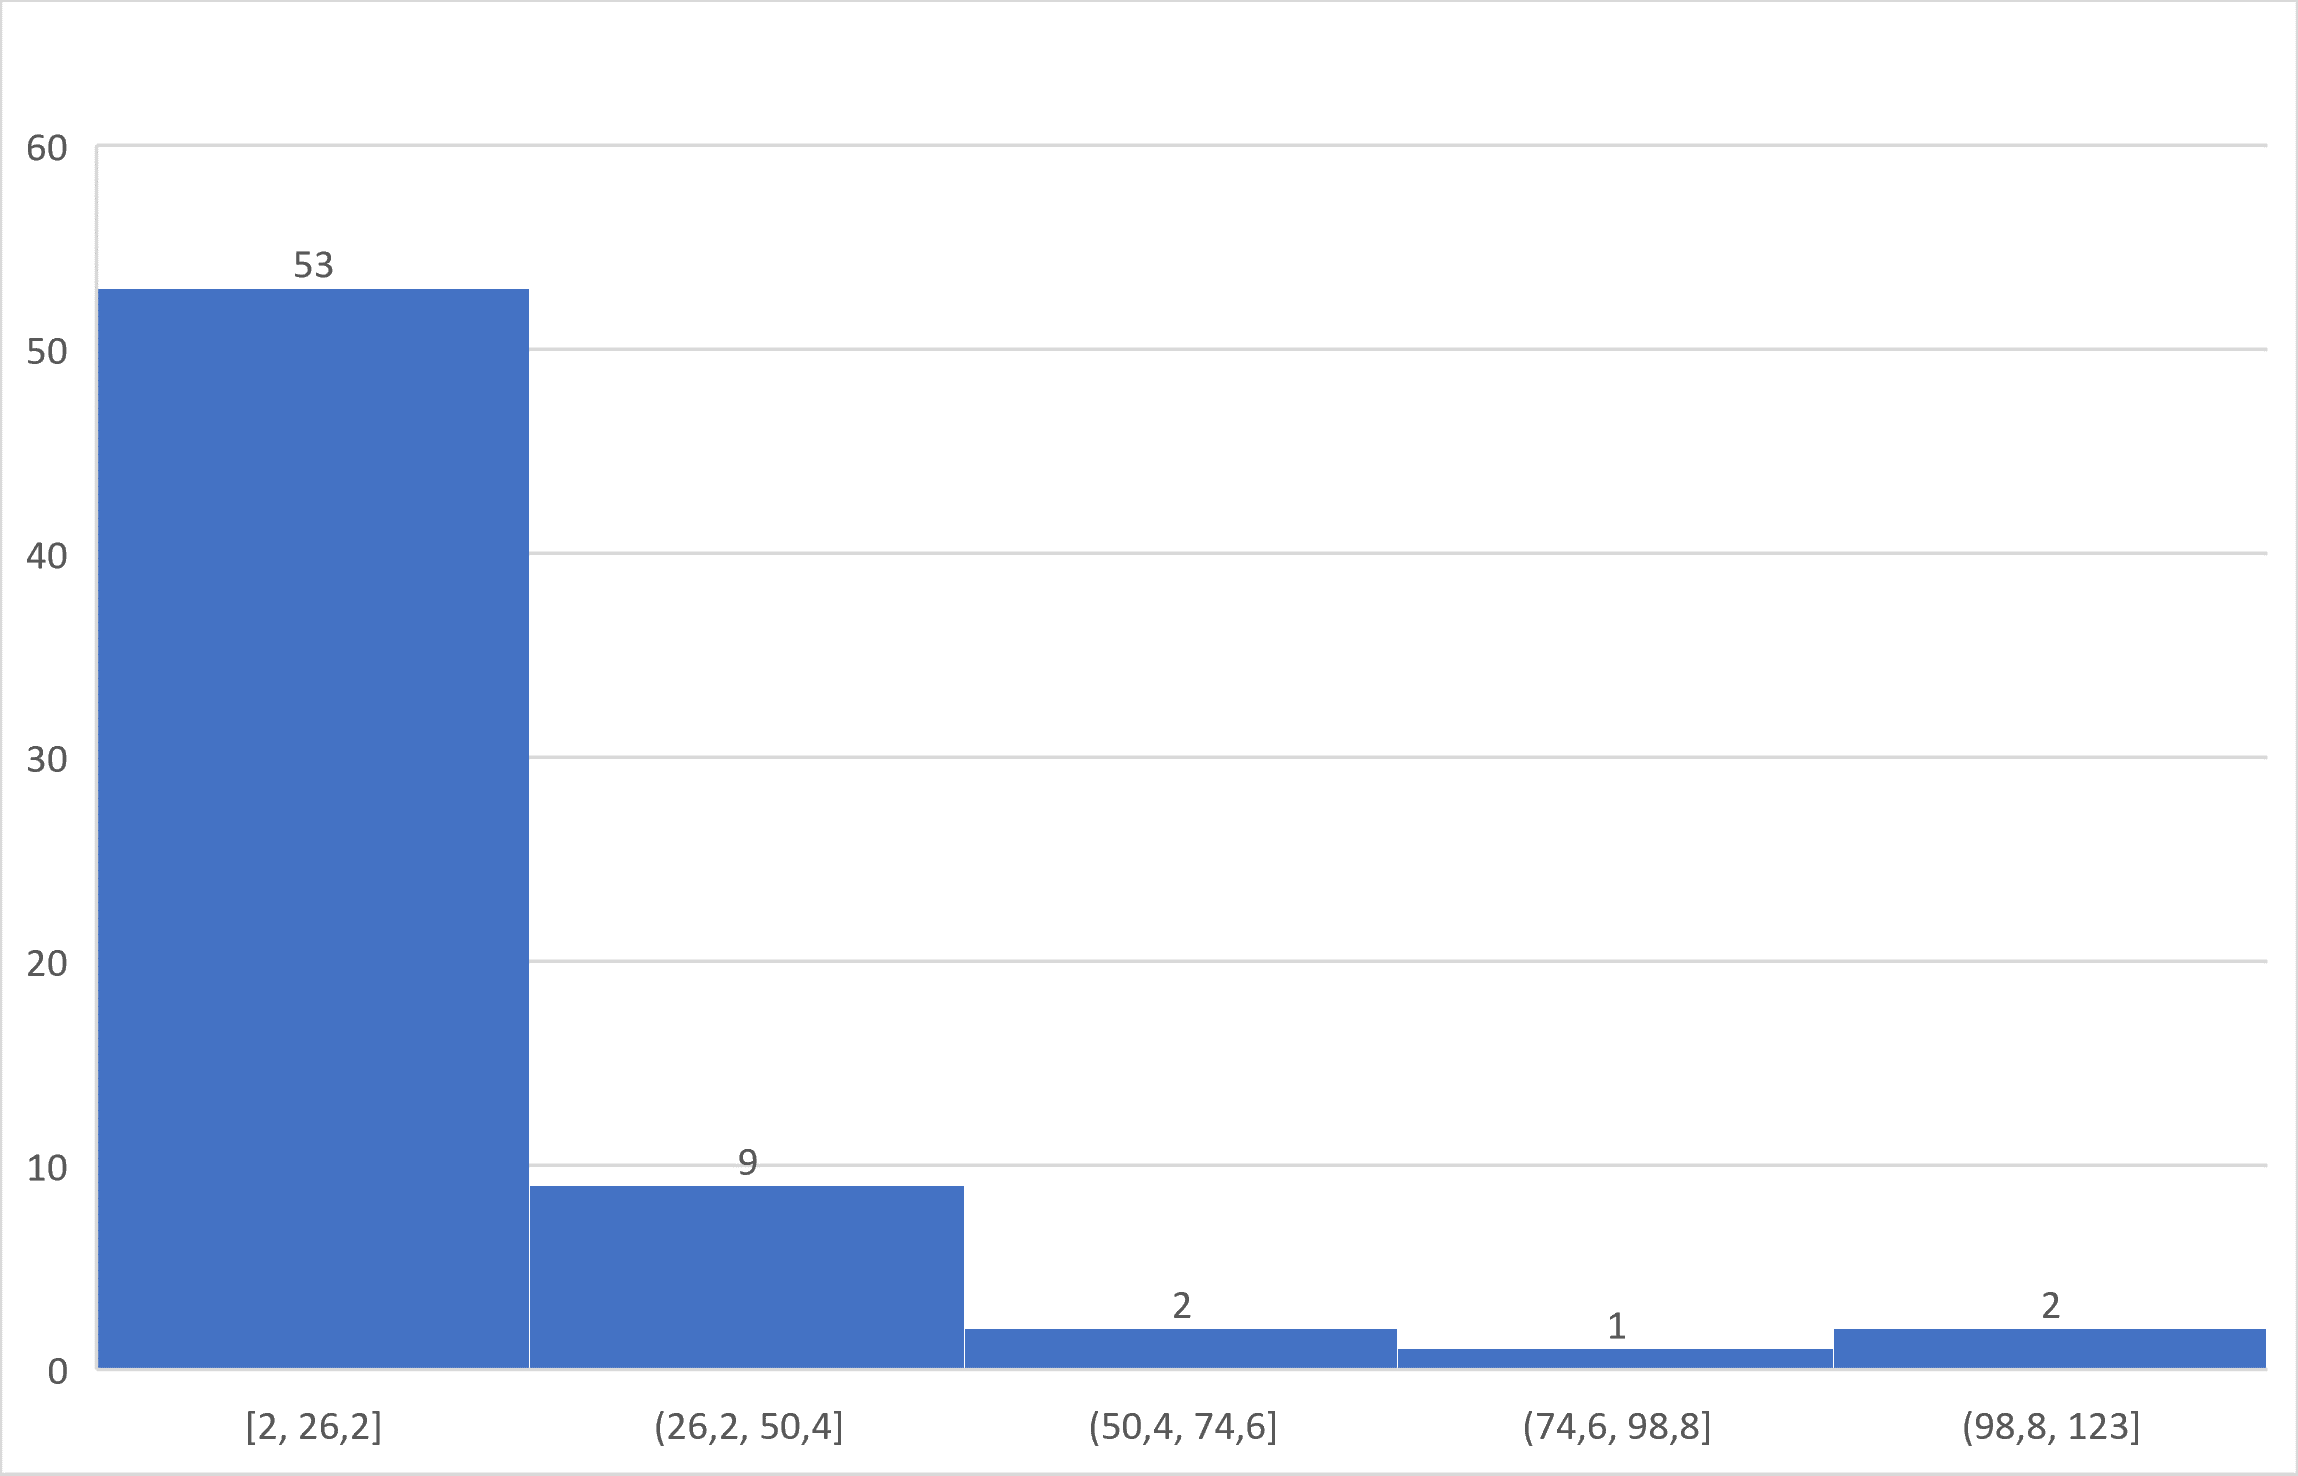
\includegraphics[width=1\textwidth]{images/vue/vue1-hist.png}
    \caption{Fájlonkénti változtatások számának a hisztogramja}
    \label{fig:vue1-hist}
\end{figure}

A \ref{fig:vue1-cov-changes} ábra mutatja a teljes repository-n a fájlonkénti változtatások számát csökkenő sorrendben, illetve a másodlagos tengelyen látható a fájlonkénti coverage. A coverage egyelőre 100\% a teljes projekten. A változtatások számára illesztett görbét érdemes megjegyezni, mert visszatérő motívum lesz a többi analízis során is.

A \ref{fig:vue1-changes-lines} az egyéni fájlok változtatási számát és a fájlok méretét ábrázolja. Bár van néhány fájl, mint például a \code{vue.js} és a \code{directive.js}, amik a sok változtatás ellenére kis méretűek, a kódbázis nagy részére igaz, hogy minél több módosítás tartozik egy fájlhoz, annál nagyobb -- számszerűsítve a korreláció a két adatsor között 0,59 a vue 1.0 esetében.

\begin{figure}[H]
    \centering
    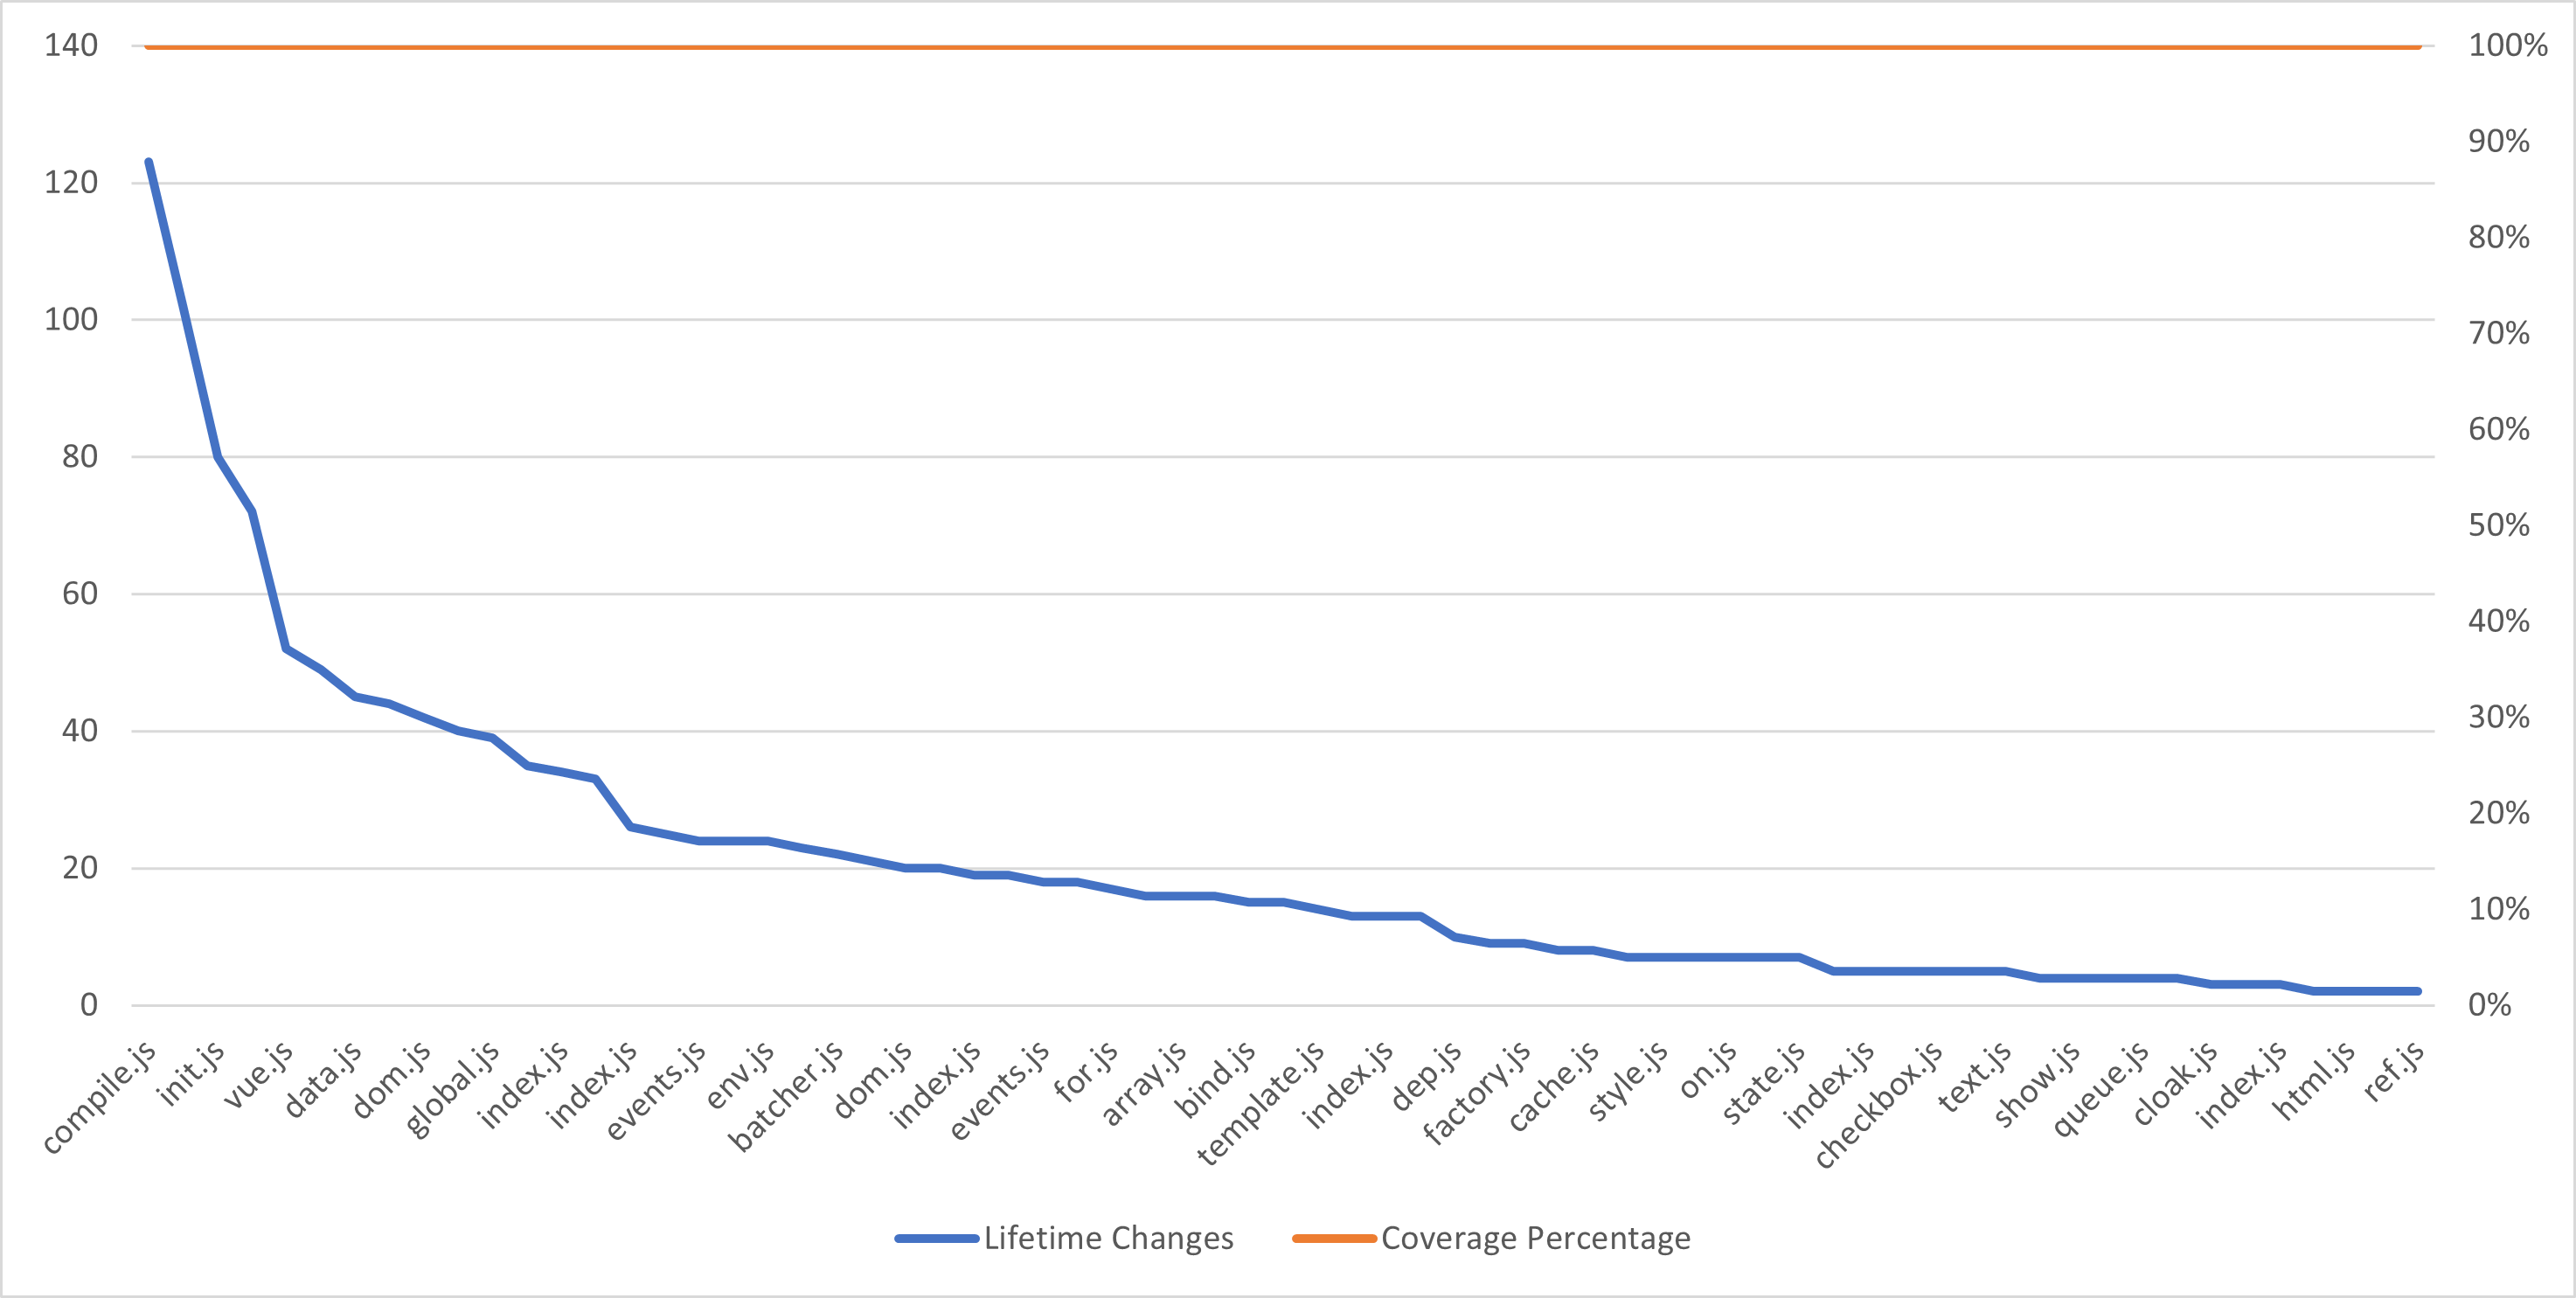
\includegraphics[width=1\textwidth]{images/vue/vue1-lifetime-changes.png}
    \caption{A coverage és az összes változtatások számának alakulása a vue 1.0 esetében}
    \label{fig:vue1-cov-changes}
\end{figure}

\begin{figure}[H]
    \centering
    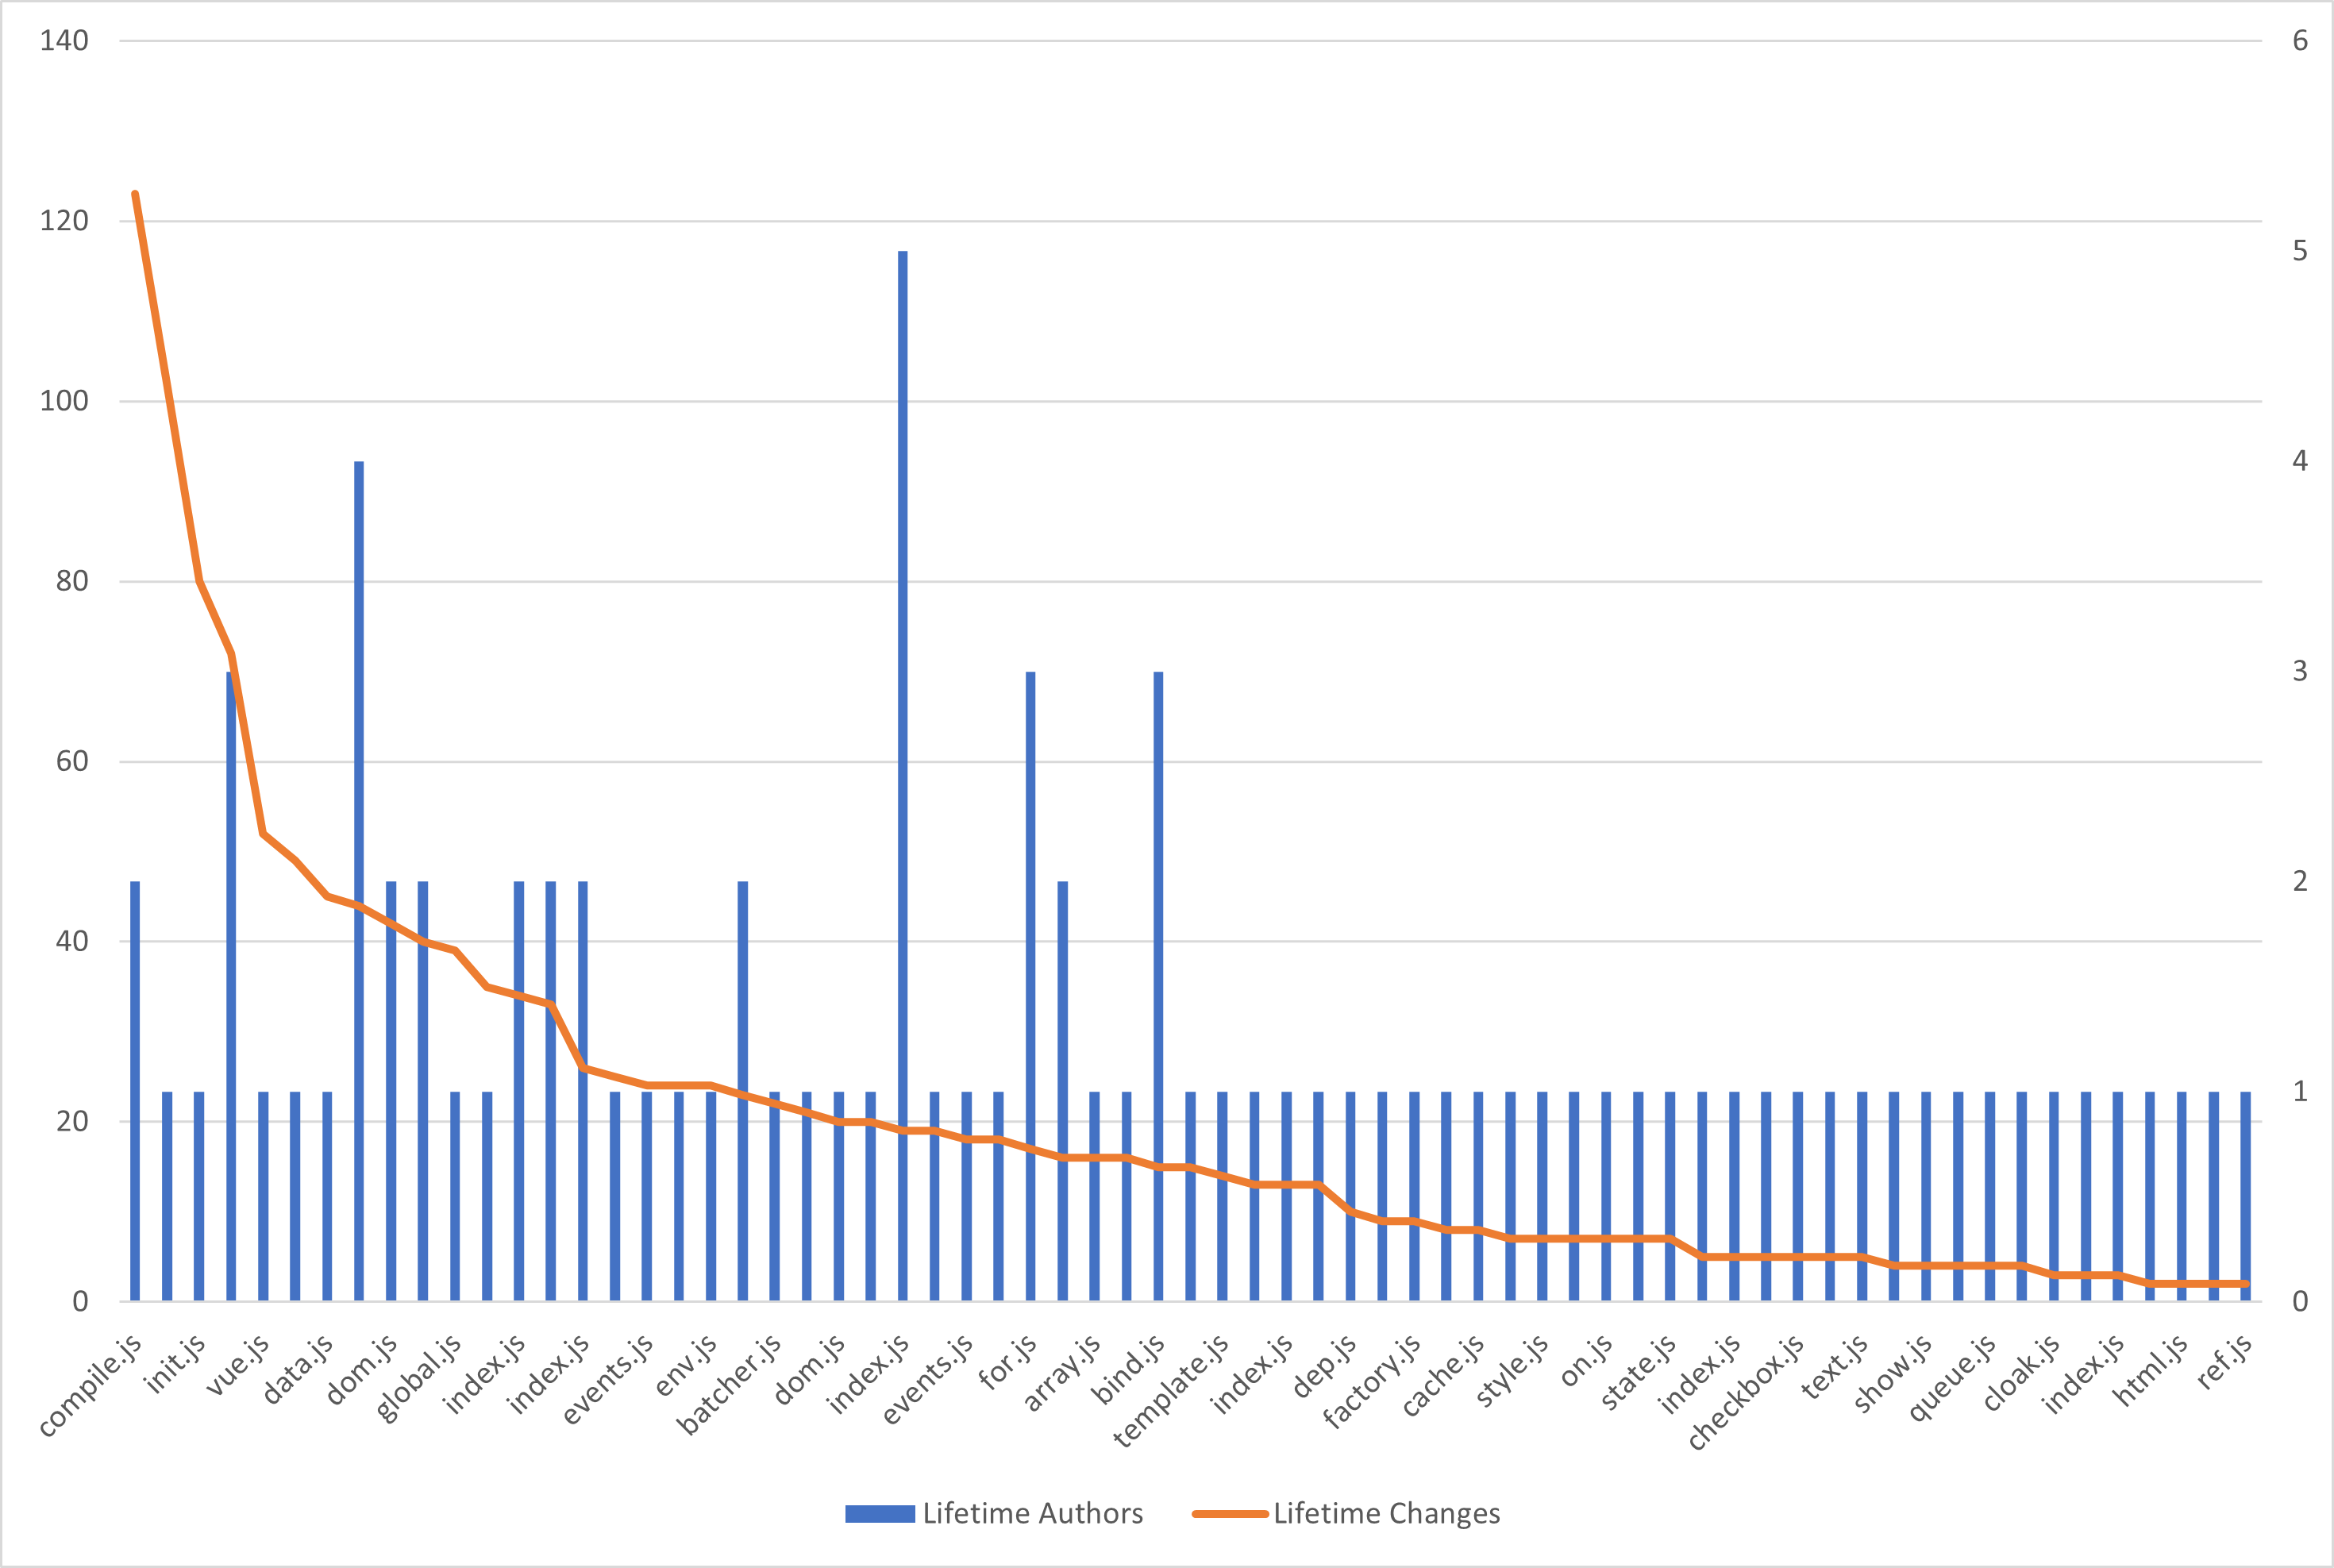
\includegraphics[width=1\textwidth]{images/vue/vue1-lifetimechanges-authors.png}
    \caption{Fájlok módosítási számai és egyedi szerzőinek száma a vue 1.0 esetében}
    \label{fig:vue1-changes-authors}
\end{figure}

Végezetül a \ref{fig:vue1-changes-authors} ábra a fájlok változtatási számát és az egyedi szerzők számát mutatja. A vue ebből a szempontból különleges eset, mert ahogy a \ref{code:vue-authors} kimenetén láttuk a projekt jelentős részben egy fejlesztő kezében van és ez kiemelten igaz az 1.0-ra. A két adatsor között a vue 1.0 esetében a korreláció 0,27.

\begin{figure}[H]
    \centering
    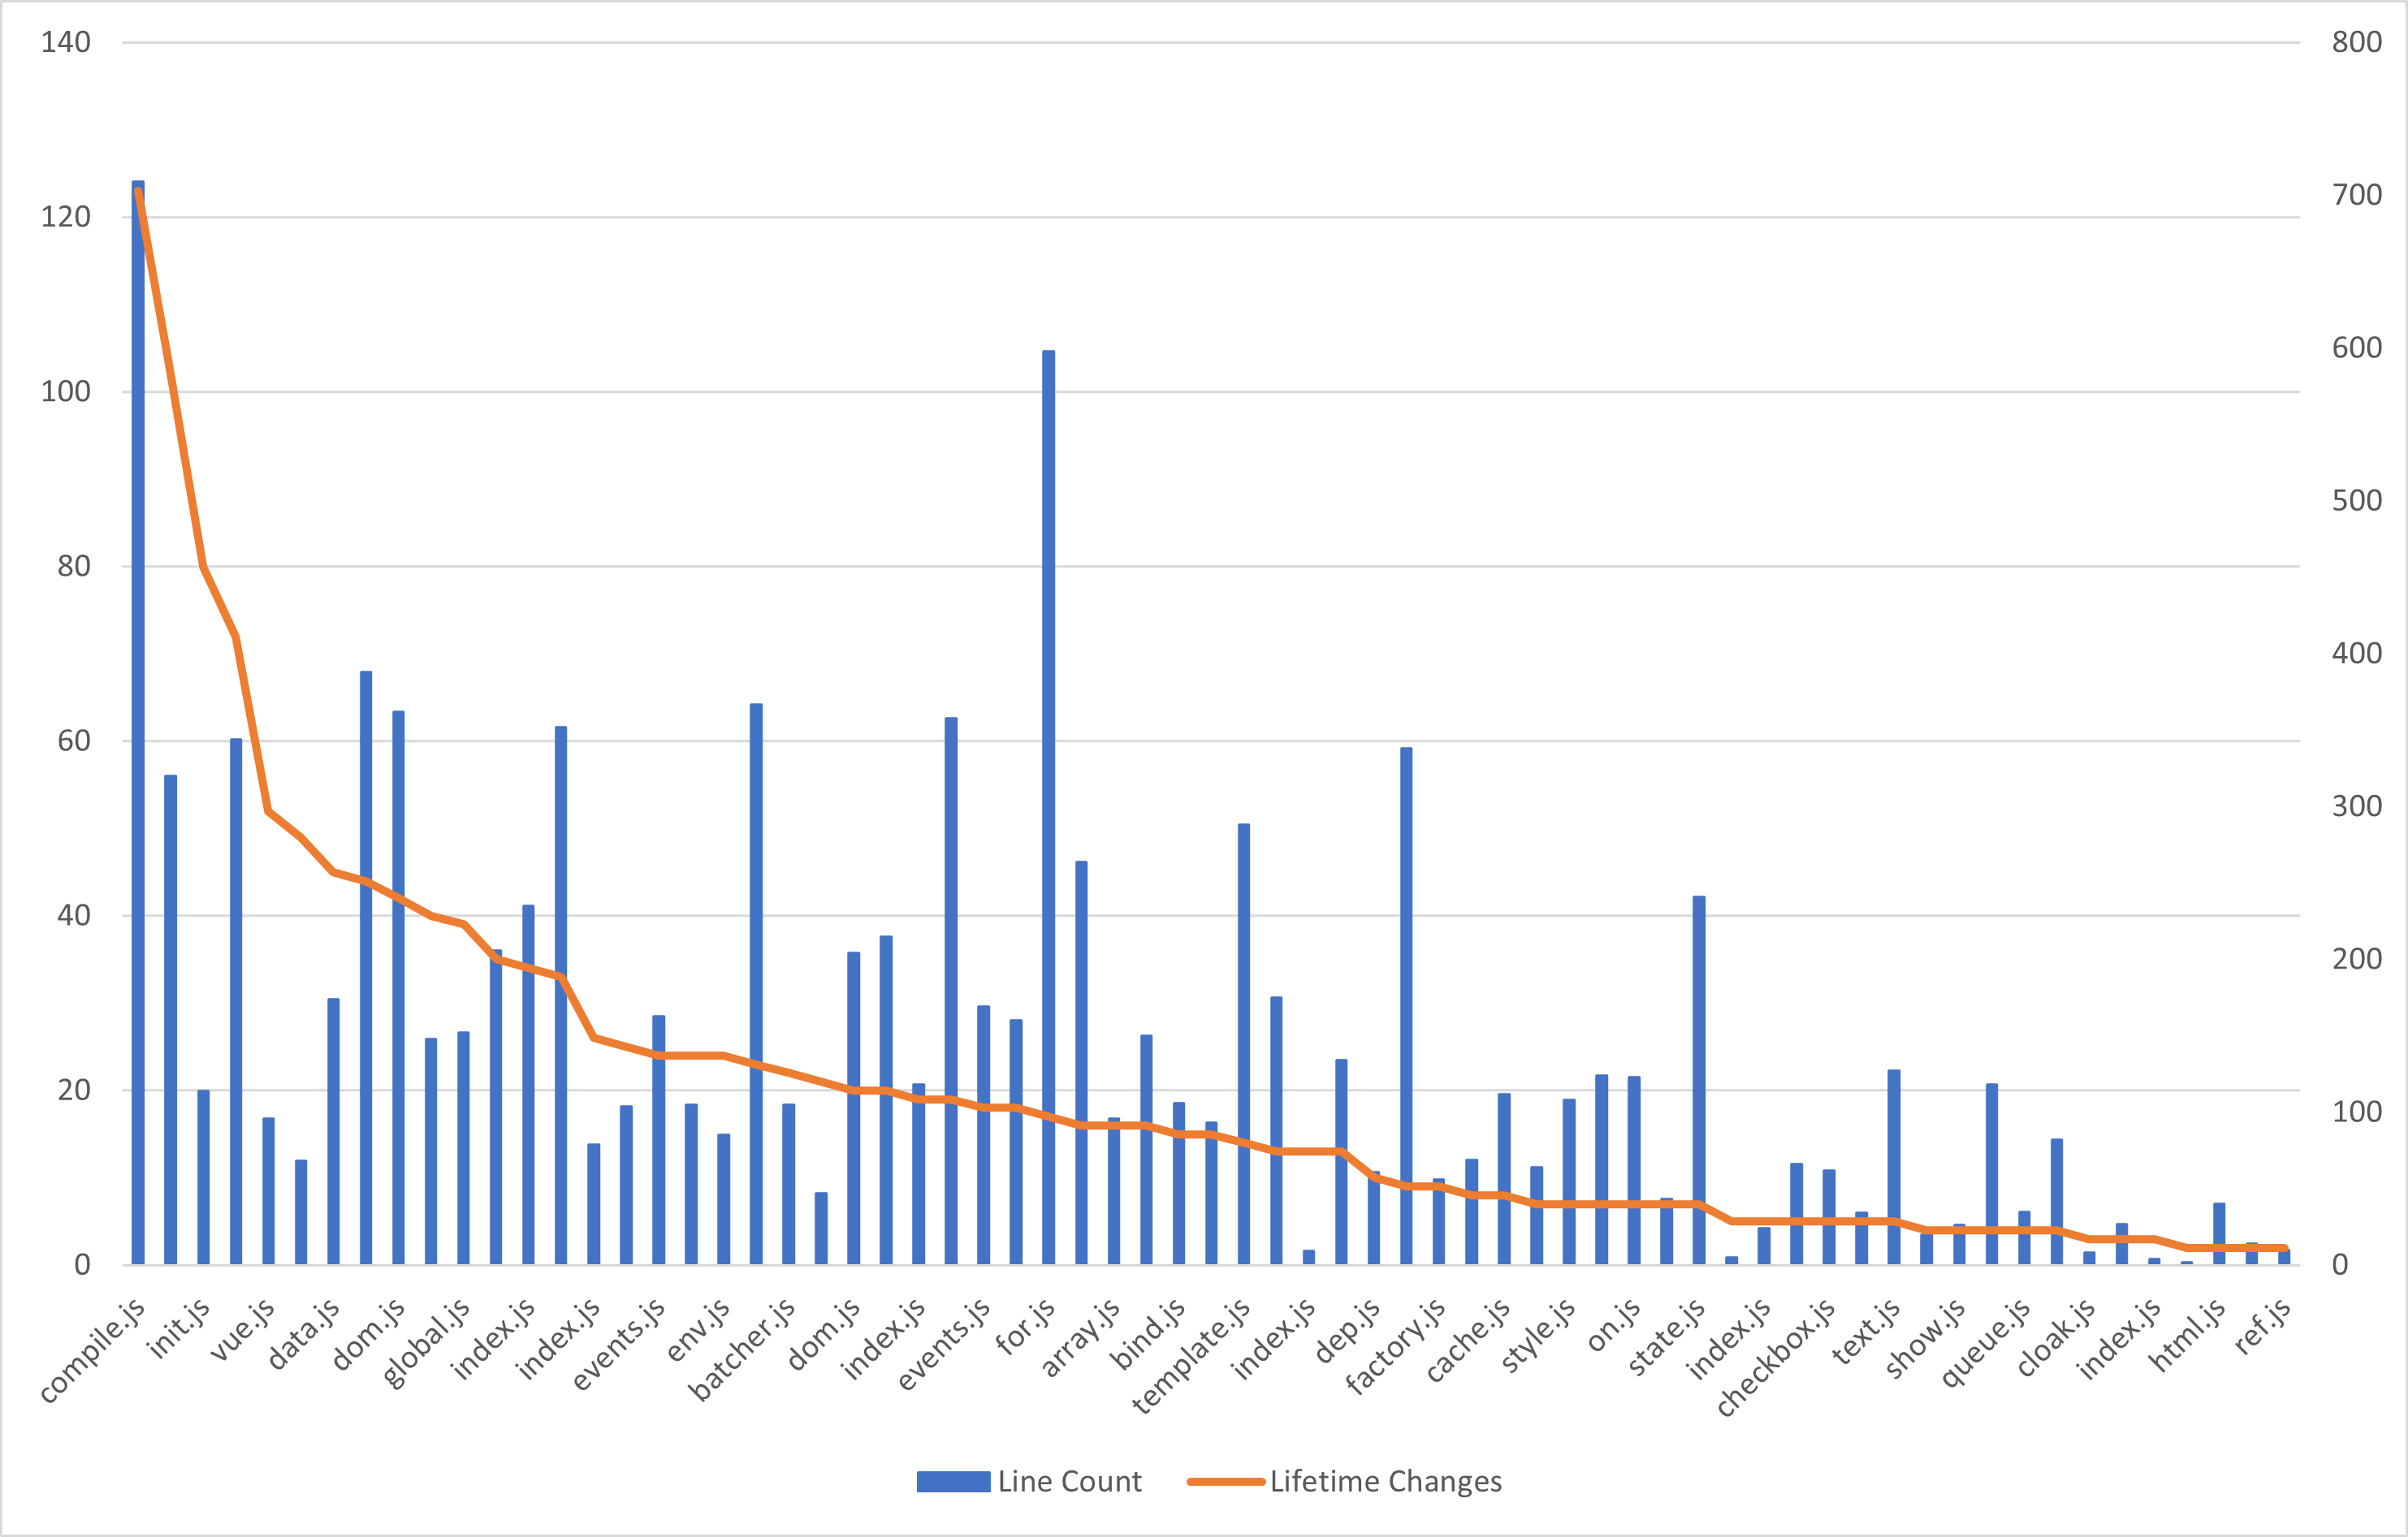
\includegraphics[width=1\textwidth]{images/vue/vue1-lines-lifetimechanges.png}
    \caption{Fájlok módosítási számai és méretük a vue 1.0 esetében}
    \label{fig:vue1-changes-lines}
\end{figure}

\pagebreak

\subsection{Vue 2.0}

A vue 2.0 alig több, mint egy évvel a vue 1.0 után jelent meg, azonban teljes újraírása volt a projektnek, így az 1.0-ban látott adatokkal csak néhány esetben fogunk tudni párhuzamot vonni. A \ref{table:vue2-top-files} táblázat mutatja, hogy a vue 2.0 esetében melyek a legtöbbet változtatott fájlok.

Külön felhívnám a figyelmet a \code{compiler/parser/index.js} és \code{compiler/codegen/index.js} fájlokra és nem csak azért, mert ez a két legtöbbet változtatott fájl. Ezek a fájlok ismerősek lehetnek a vue 1.0-nál látott \code{compile.js} miatt, ami mint az látható a \ref{table:vue1-top-files} táblázatból az akkori állapot legtöbbet változtatott fájlja. Ugyan a git szempontjából nincs kapcsolat a \code{compile.js}, \code{compiler/parser/index.js} és \code{compiler/codegen/index.js} fájlok között, ránézésre azonban hamar kiderül, hogy a \code{compile.js} tovább él a 2.0-ban, két külön fájlra bontva. Ez már most egy érdekes trendet mutat: hiába lett refactor-olva a \code{compile.js}, a szétbontott fájlok pontosan ugyanazt a mintát mutatják, mint az elődjük.

\begin{table}[h]
    \hspace*{-1cm}\begin{tabular}{l|l|l|l|l}
        Filename                     & Lifetime Authors & Lifetime Changes & Line Count & Coverage \% \\ \hline
        compiler/parser/index.js     & 5                & 93               & 467        & 100         \\
        compiler/codegen/index.js    & 2                & 72               & 246        & 100         \\
        render.js                    & 2                & 67               & 253        & 100         \\
        create-component.js          & 4                & 56               & 296        & 100         \\
        patch.js                     & 2                & 54               & 524        & 100         \\
        transition.js                & 1                & 47               & 270        & 100         \\
        lifecycle.js                 & 3                & 45               & 201        & 100         \\
        helpers.js                   & 2                & 34               & 145        & 100         \\
        web-runtime-with-compiler.js & 3                & 33               & 84         & 100         \\
        core/index.js                & 1                & 31               & 13         & 100
    \end{tabular}
    \caption{A vue 2.0-ás kiadásának leggyakrabban módosított fájljai} \label{table:vue2-top-files}
\end{table}

A \code{compile.js} utódait leszámítva azonban a vue 2.0 kódbázisa a \ref{fig:vue2-lifetime-changes} ábra alapján kevésbé polarizált fájl módosítási számok tekintetében, mint a 1.0-ás kiadásban volt. Azt nehéz viszont megítélni, hogy ez fedi-e a valóságot, vagy csak a git technikalitása a teljes újraírás miatt, hiszen láttuk, hogy a \code{compile.js} két utódja teljesen tiszta lappal indult és ugyanez a minta előfordulhat kevésbé egyértelmű szituációkban is.

\begin{figure}[H]
    \centering
    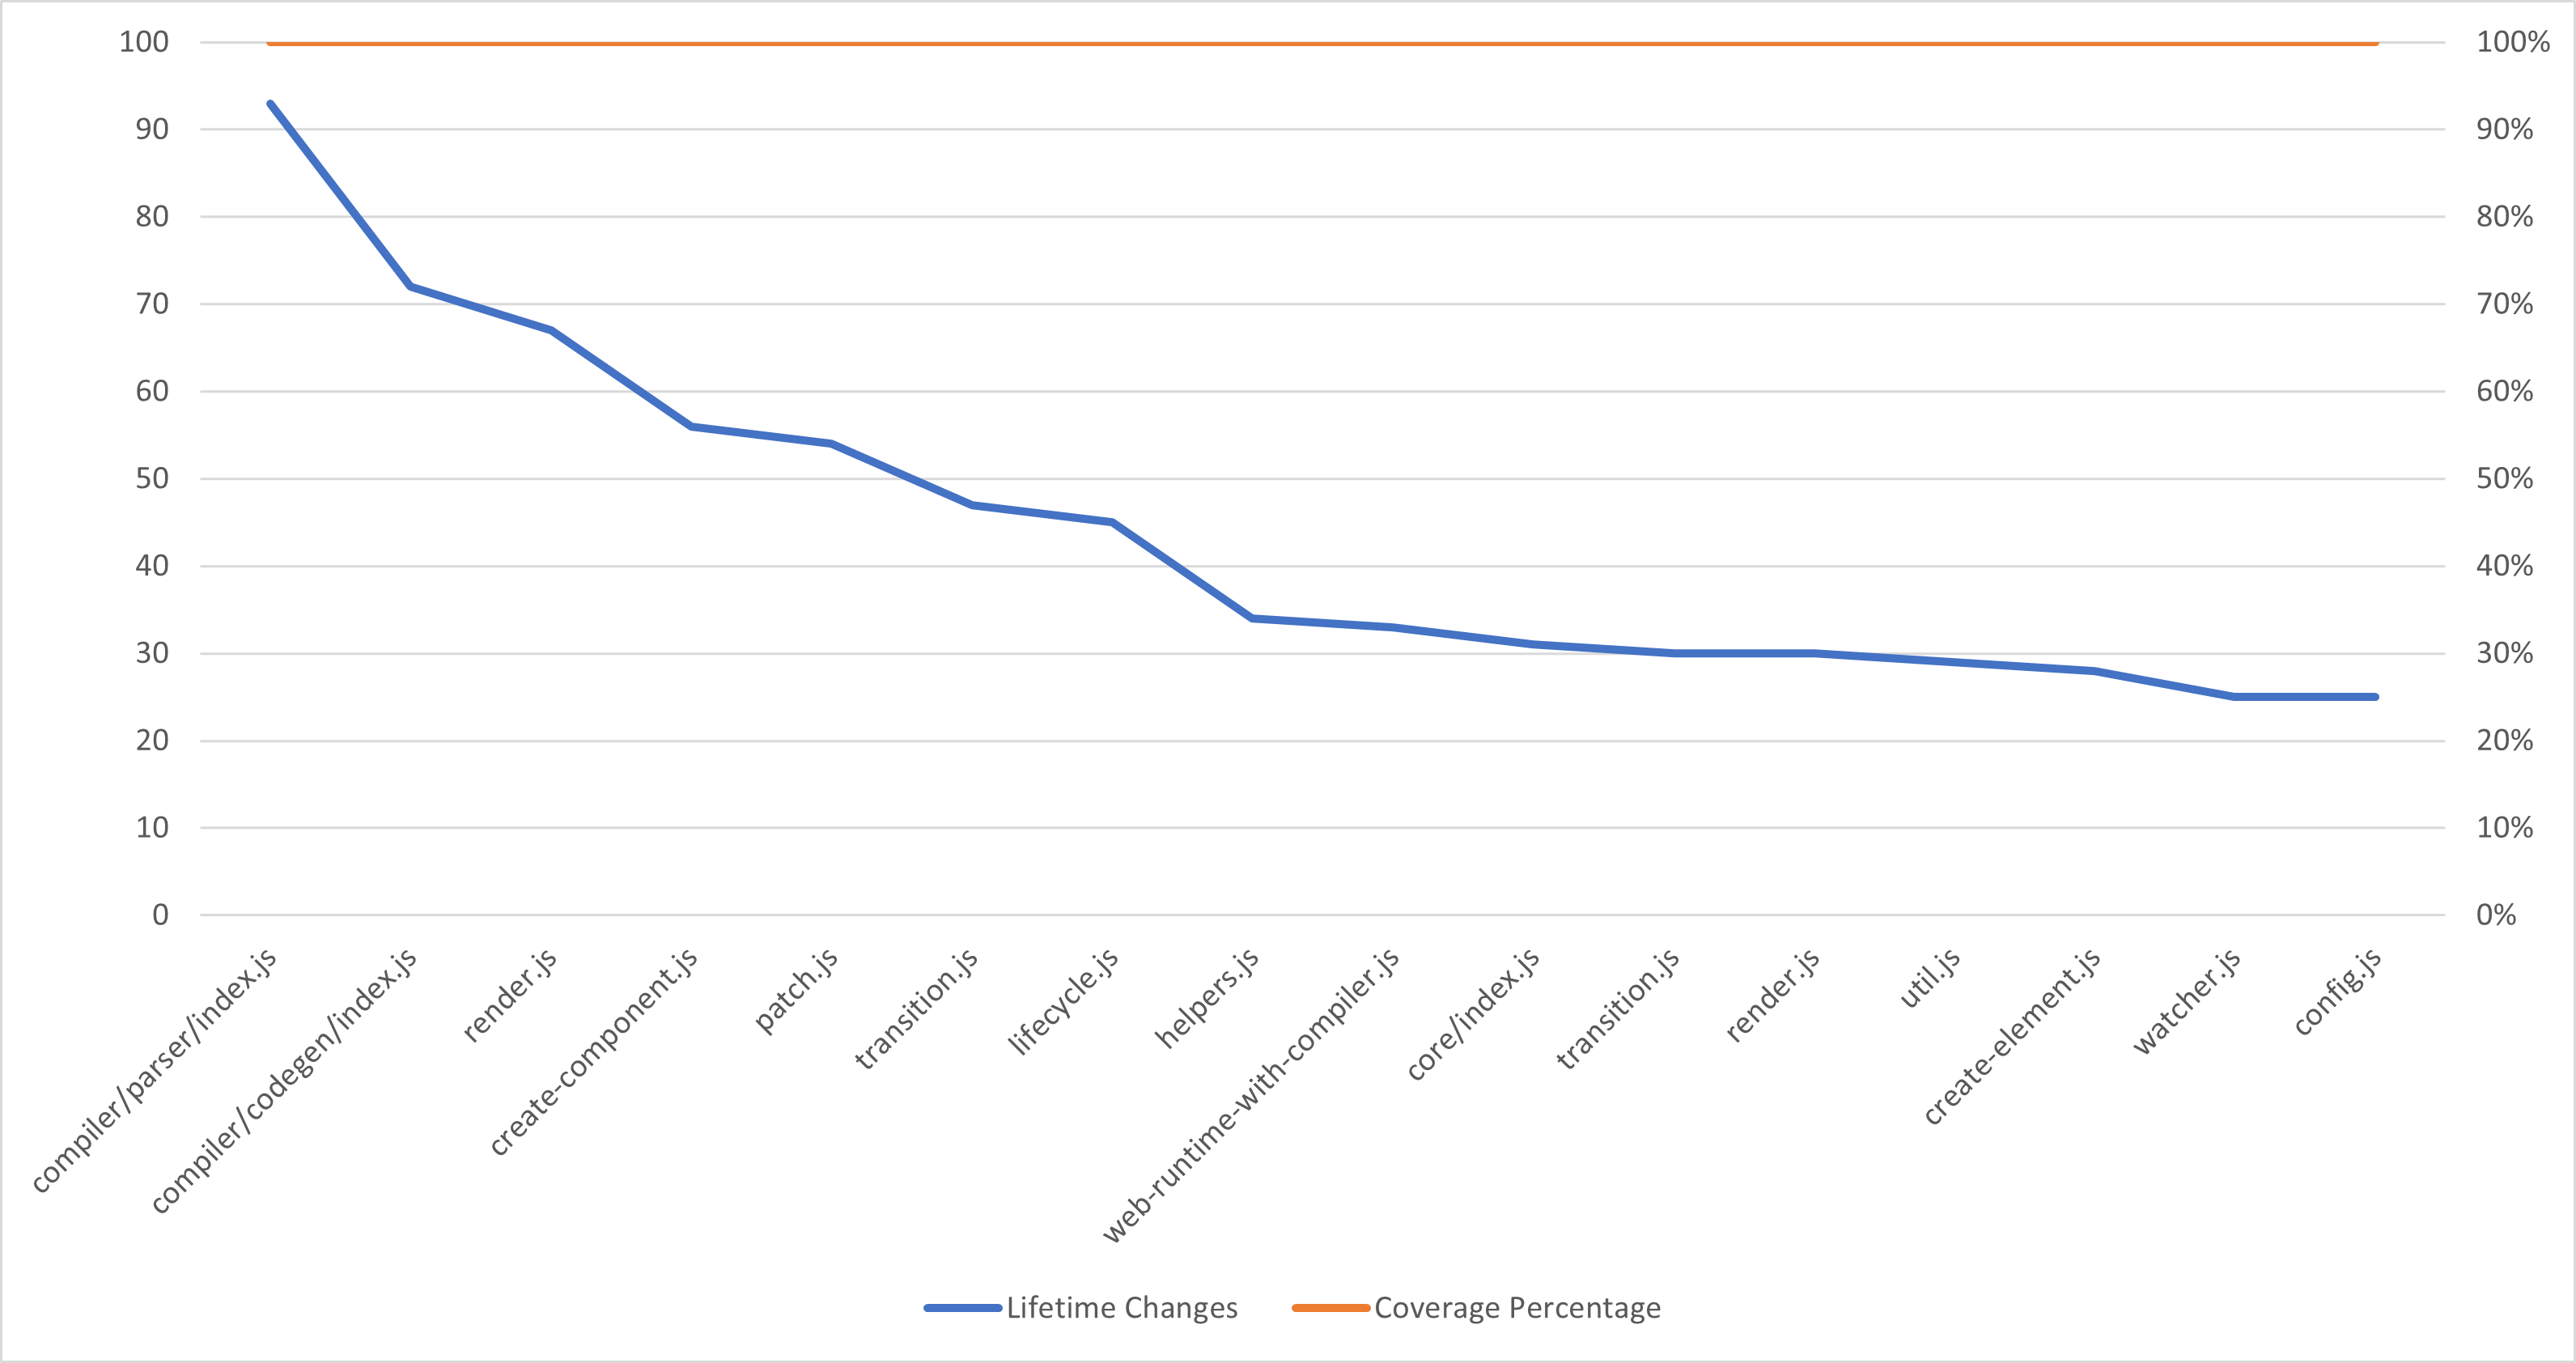
\includegraphics[width=1\textwidth]{images/vue/vue2-lifetime-changes.png}
    \caption{Fájlok módosítási számai a vue 2.0.1 esetében}
    \label{fig:vue2-lifetime-changes}
\end{figure}

A módosítási számok hisztogramja a \ref{fig:vue2-hist} nagyon hasonló képet fest a korábbiakban látottakhoz. A 2.0 kódbázisának túlnyomó többsége ismét a ritkán módosított fájlokba tömörül, azonban a leggyakrabban módosított felső 10\% újfent az átlagos módosítási szám sokszorosát produkálja.

\begin{figure}[H]
    \centering
    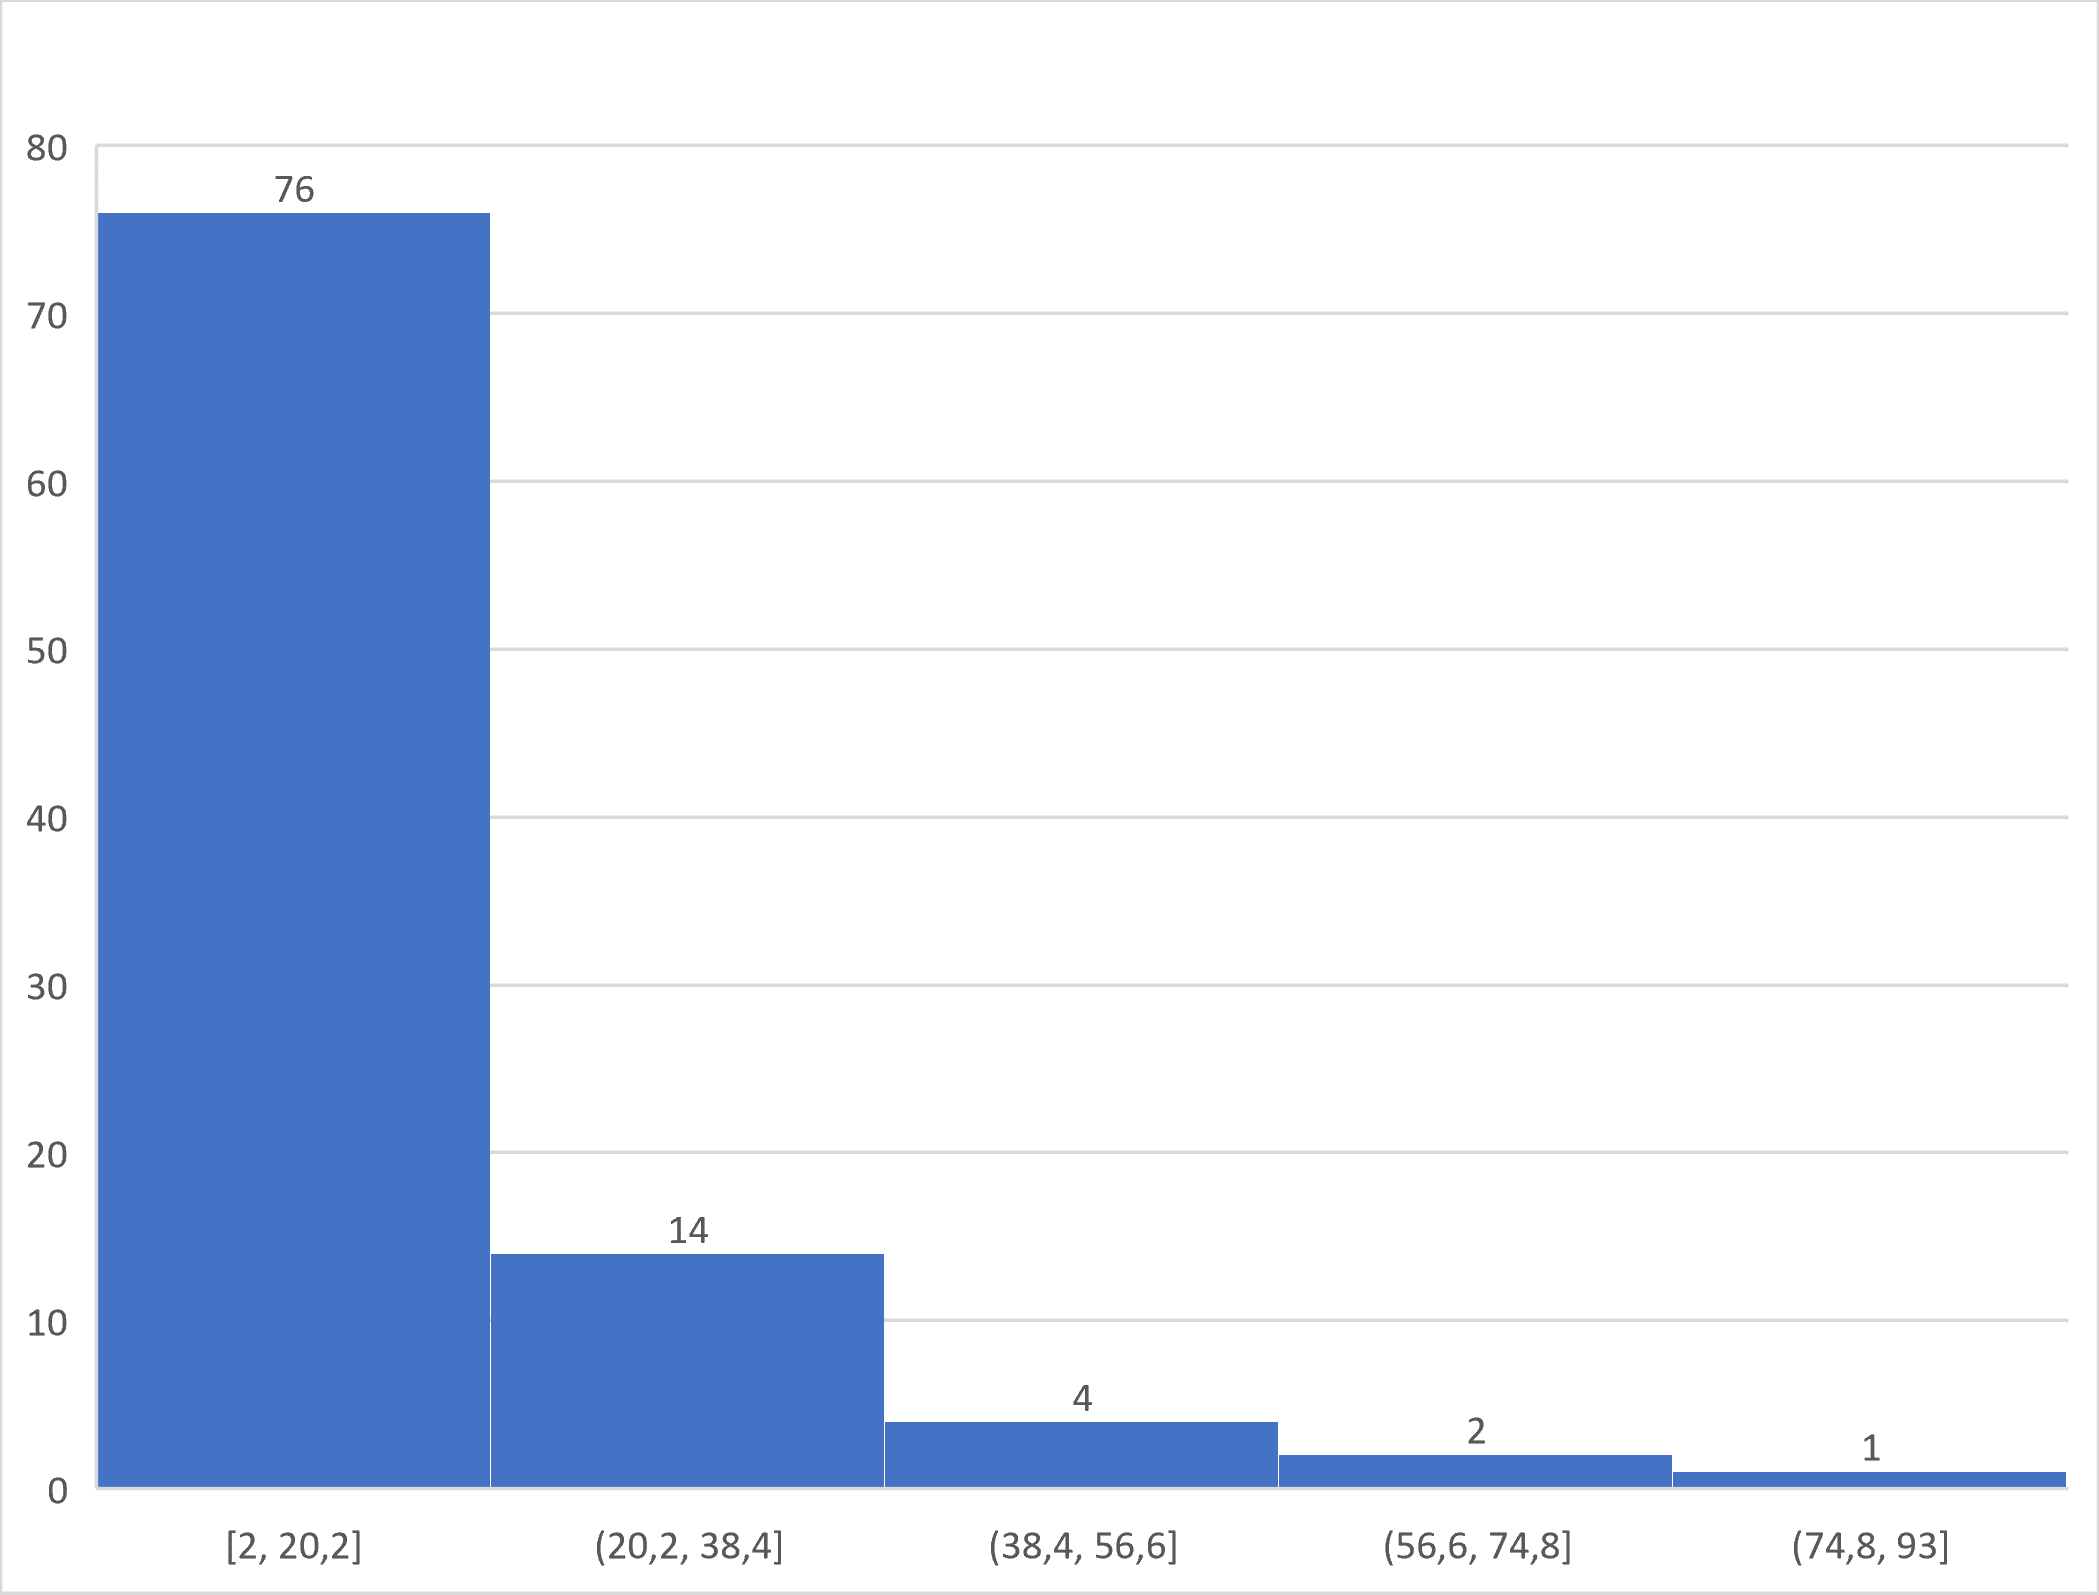
\includegraphics[width=1\textwidth]{images/vue/vue2-hist.png}
    \caption{Fájlok módosítási számának hisztogramja a vue 2.0.1 esetében}
    \label{fig:vue2-hist}
\end{figure}

Végül vegyük szemre a \ref{fig:vue2-lines-changes} ábrát, ami a fájlok módosítási számait és méretét mutatja. Ellentétben az 1.0-ban látottakkal, a 2.0 kódbázisa esetében a fájlok méretéből rajzolt görbe sokkal közelebb követi le a módosítási számokból rajzolt görbét.

\begin{figure}[H]
    \centering
    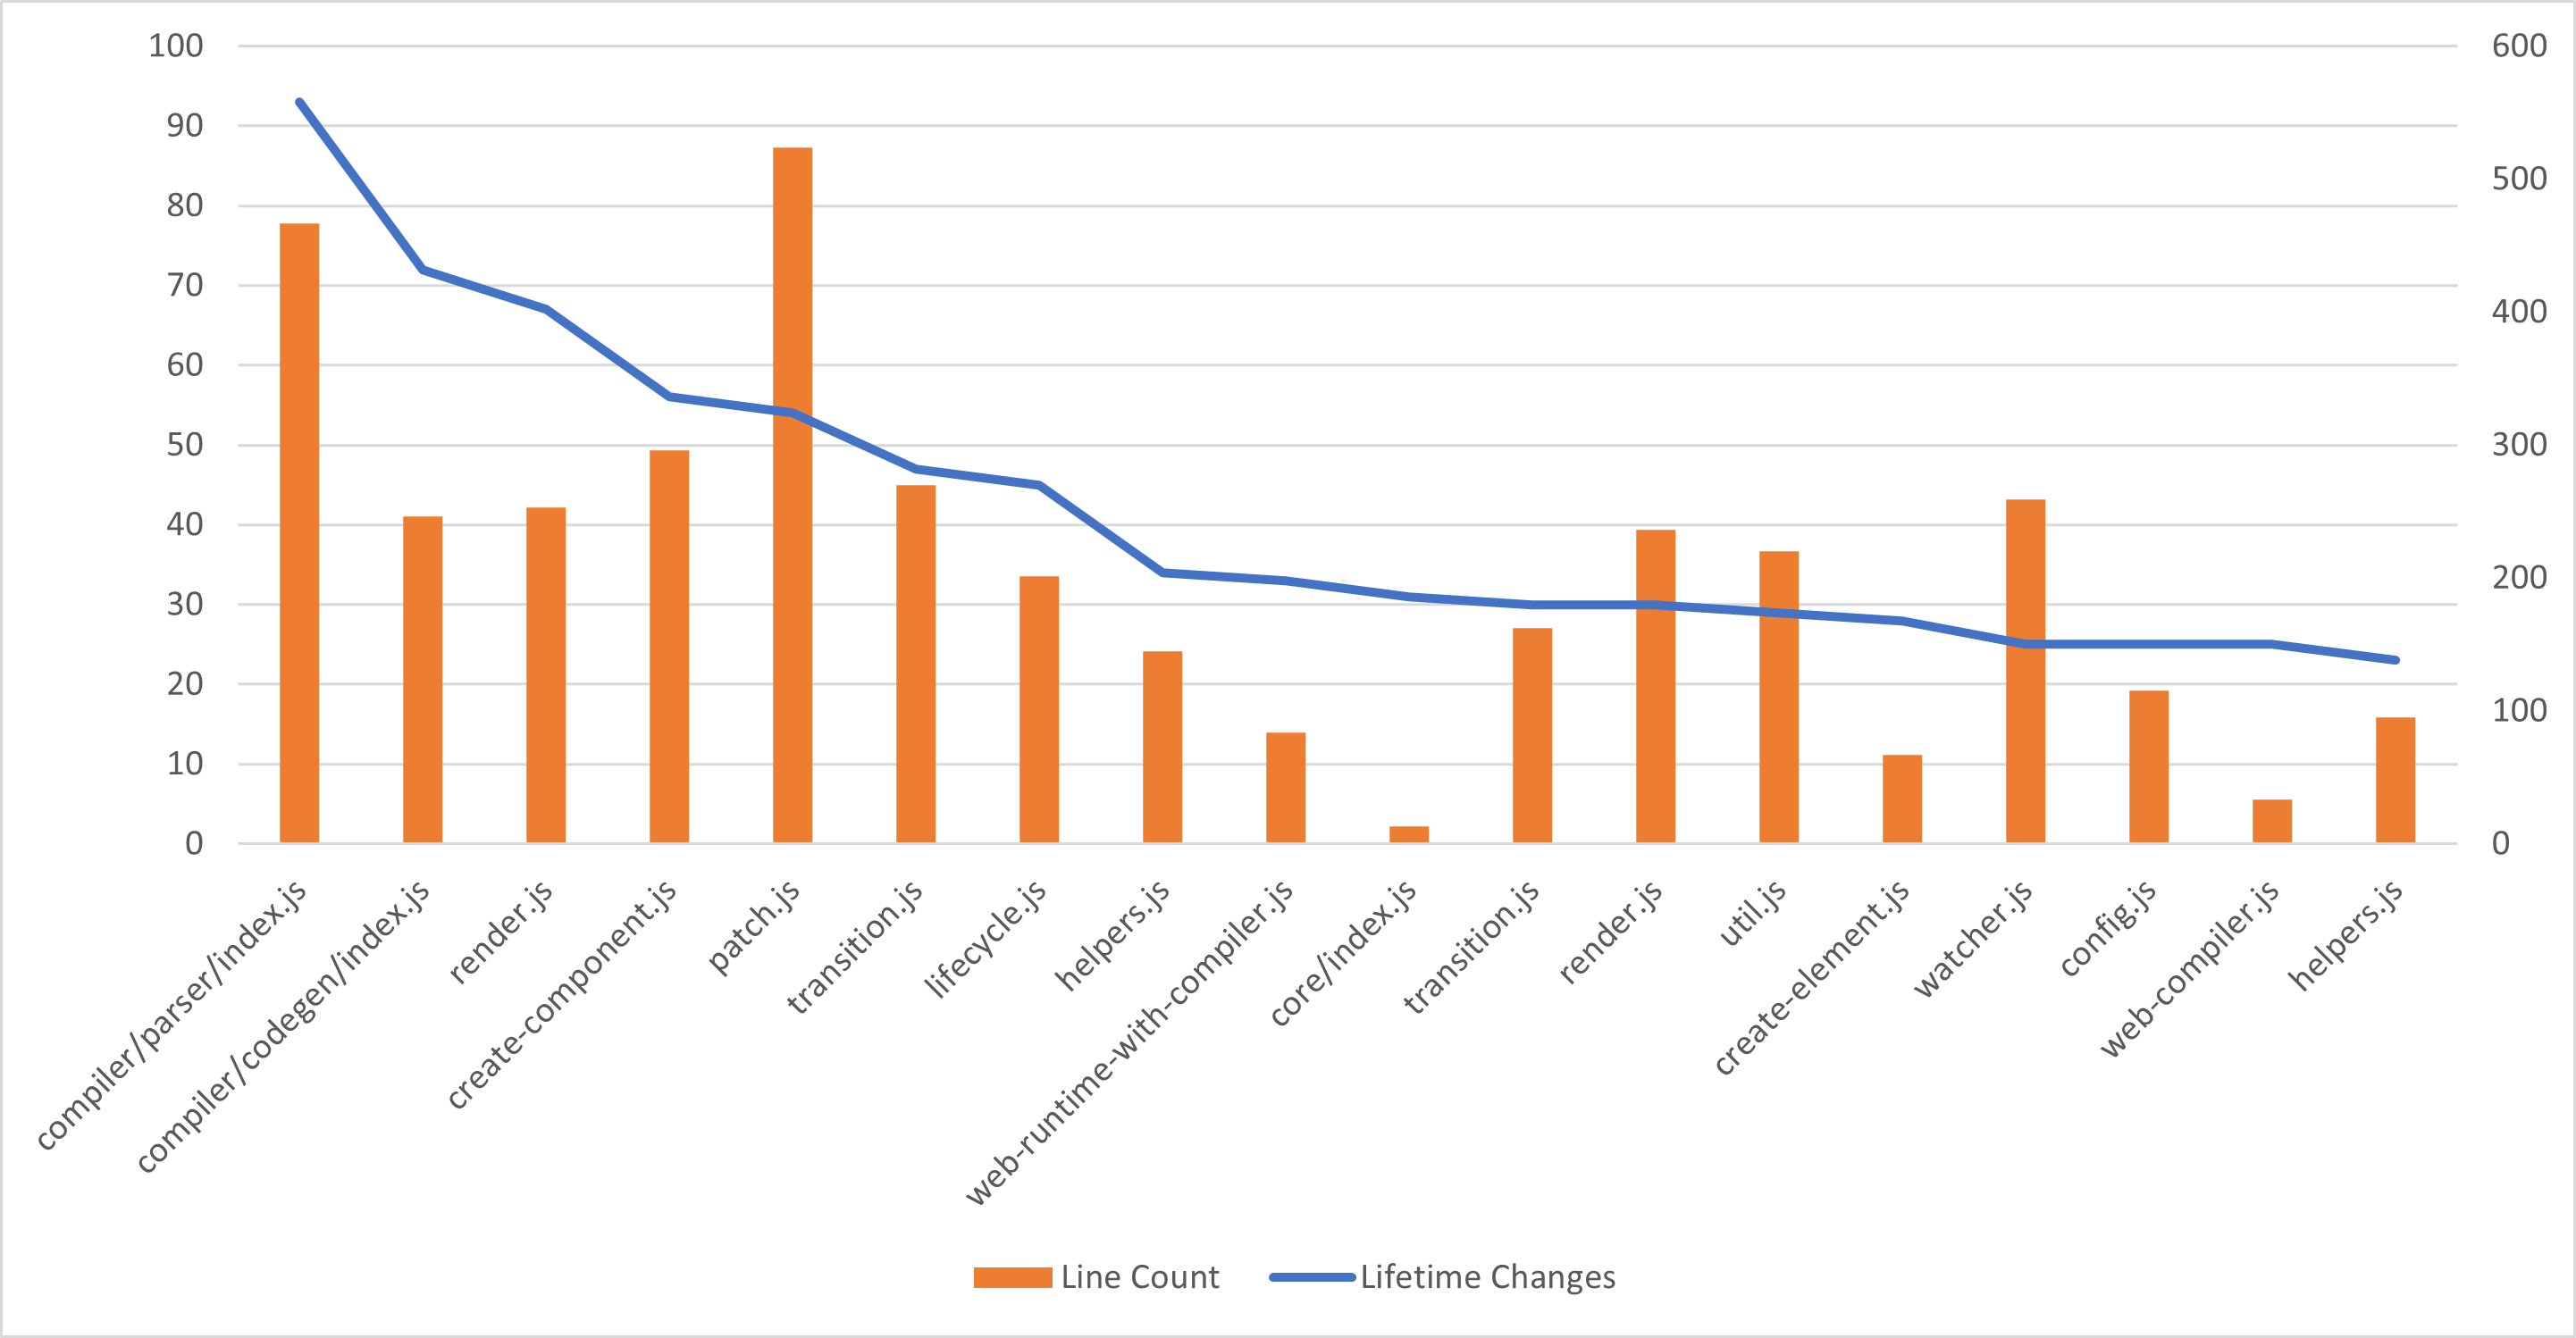
\includegraphics[width=1\textwidth]{images/vue/vue2-lines-lifetimechanges.png}
    \caption{A vékony kliens által generált grafikonok}
    \label{fig:vue2-lines-changes}
\end{figure}

\subsection{Trendek a vue 2.0, 2.4 és a legfrissebb verzió között}

Mielőtt levonnánk néhány tanulságot, nézzük meg, hogy hogyan alakult a vue kódbázisa a 2016-ban megjelent 2.0-ás verzió és a jelenlegi, 2020-as éles verzió között. A \ref{tab:vue-changes-comp} táblázat mutatja a fájlok módosítási számát 2.0.1 és a legfrissebb verzió között, a 2.0.1-es változtatási szám szerinti csökkenő sorrendben. Ugyan ez a táblázat csak a top 10 fájlt mutatja, de itt is egyértelműen látszódik egy trend, ami egyébként a teljes, 90 fájlból álló kódbázisra is igaz: ha egy fájlt sokat kellett módosítani a projekt életciklusának elején, akkor sokat kellett módosítani később is, amíg a keveset változtatott fájlok jellemzően kevés változtatásra szorulnak a teljes életciklusuk alatt. Nem meglepő módon így a korreláció a 2.0.1-es és a legfrissebb verzió változtatási számai között nagyon magas, 0,965.

\begin{table}[h]
    \centering
    \begin{tabular}{l|l|l|l|l}
        Filename                  & 2.0.1 & 2.4.0 & master & delta \\ \hline
        compiler/parser/index.js  & 93    & 149   & 206    & 113   \\
        compiler/codegen/index.js & 72    & 121   & 160    & 88    \\
        render.js                 & 67    & 105   & 122    & 55    \\
        create-component.js       & 56    & 91    & 112    & 56    \\
        patch.js                  & 54    & 92    & 119    & 65    \\
        transition.js             & 47    & 68    & 73     & 26    \\
        lifecycle.js              & 45    & 76    & 96     & 51    \\
        core/index.js             & 31    & 47    & 48     & 17    \\
        render.js                 & 30    & 60    & 72     & 42    \\
        transition.js             & 30    & 49    & 54     & 24
    \end{tabular}
    \caption{A vue.js legtöbbet változtatott fájljai 2.0 és az aktuális verzió között}
    \label{tab:vue-changes-comp}
\end{table}

A \ref{fig:vue-all-files-lifetime-changes} ábra új rendezési szempont szerint mutatja be a projekt összes fájlját módosítások száma szerint, a legújabb verzióban megfigyelt érték szerint csökkenő sorrendben. Ezen az ábrán két nagyon szembetűnő tény figyelhető meg:
\begin{itemize}
    \item A fájlok módosítási számai közötti erőviszonyok négy évnyi változtatás során sem változtak, a polarizáltság változatlanul nagyon magas
    \item Új változási gócpontot képező fájlok nem alakultak ki
\end{itemize}

A \ref{fig:vue-all-delta-hist} hisztogram a vue 2.0 és a legfrissebb verzió között megfigyelt fájl módosítások deltáit csoportosítja, azaz azt, hogy a két verzió között hány változtatás érintette az adott fájlokat. Ahogy várható, ez a hisztogram tökéletesen leköveti a 2.0-tól megfigyelt változtatási számokból képzett hisztogramokat, tovább erősítve az eddig megfigyelt trendeket.

\begin{figure}[H]
    \centering
    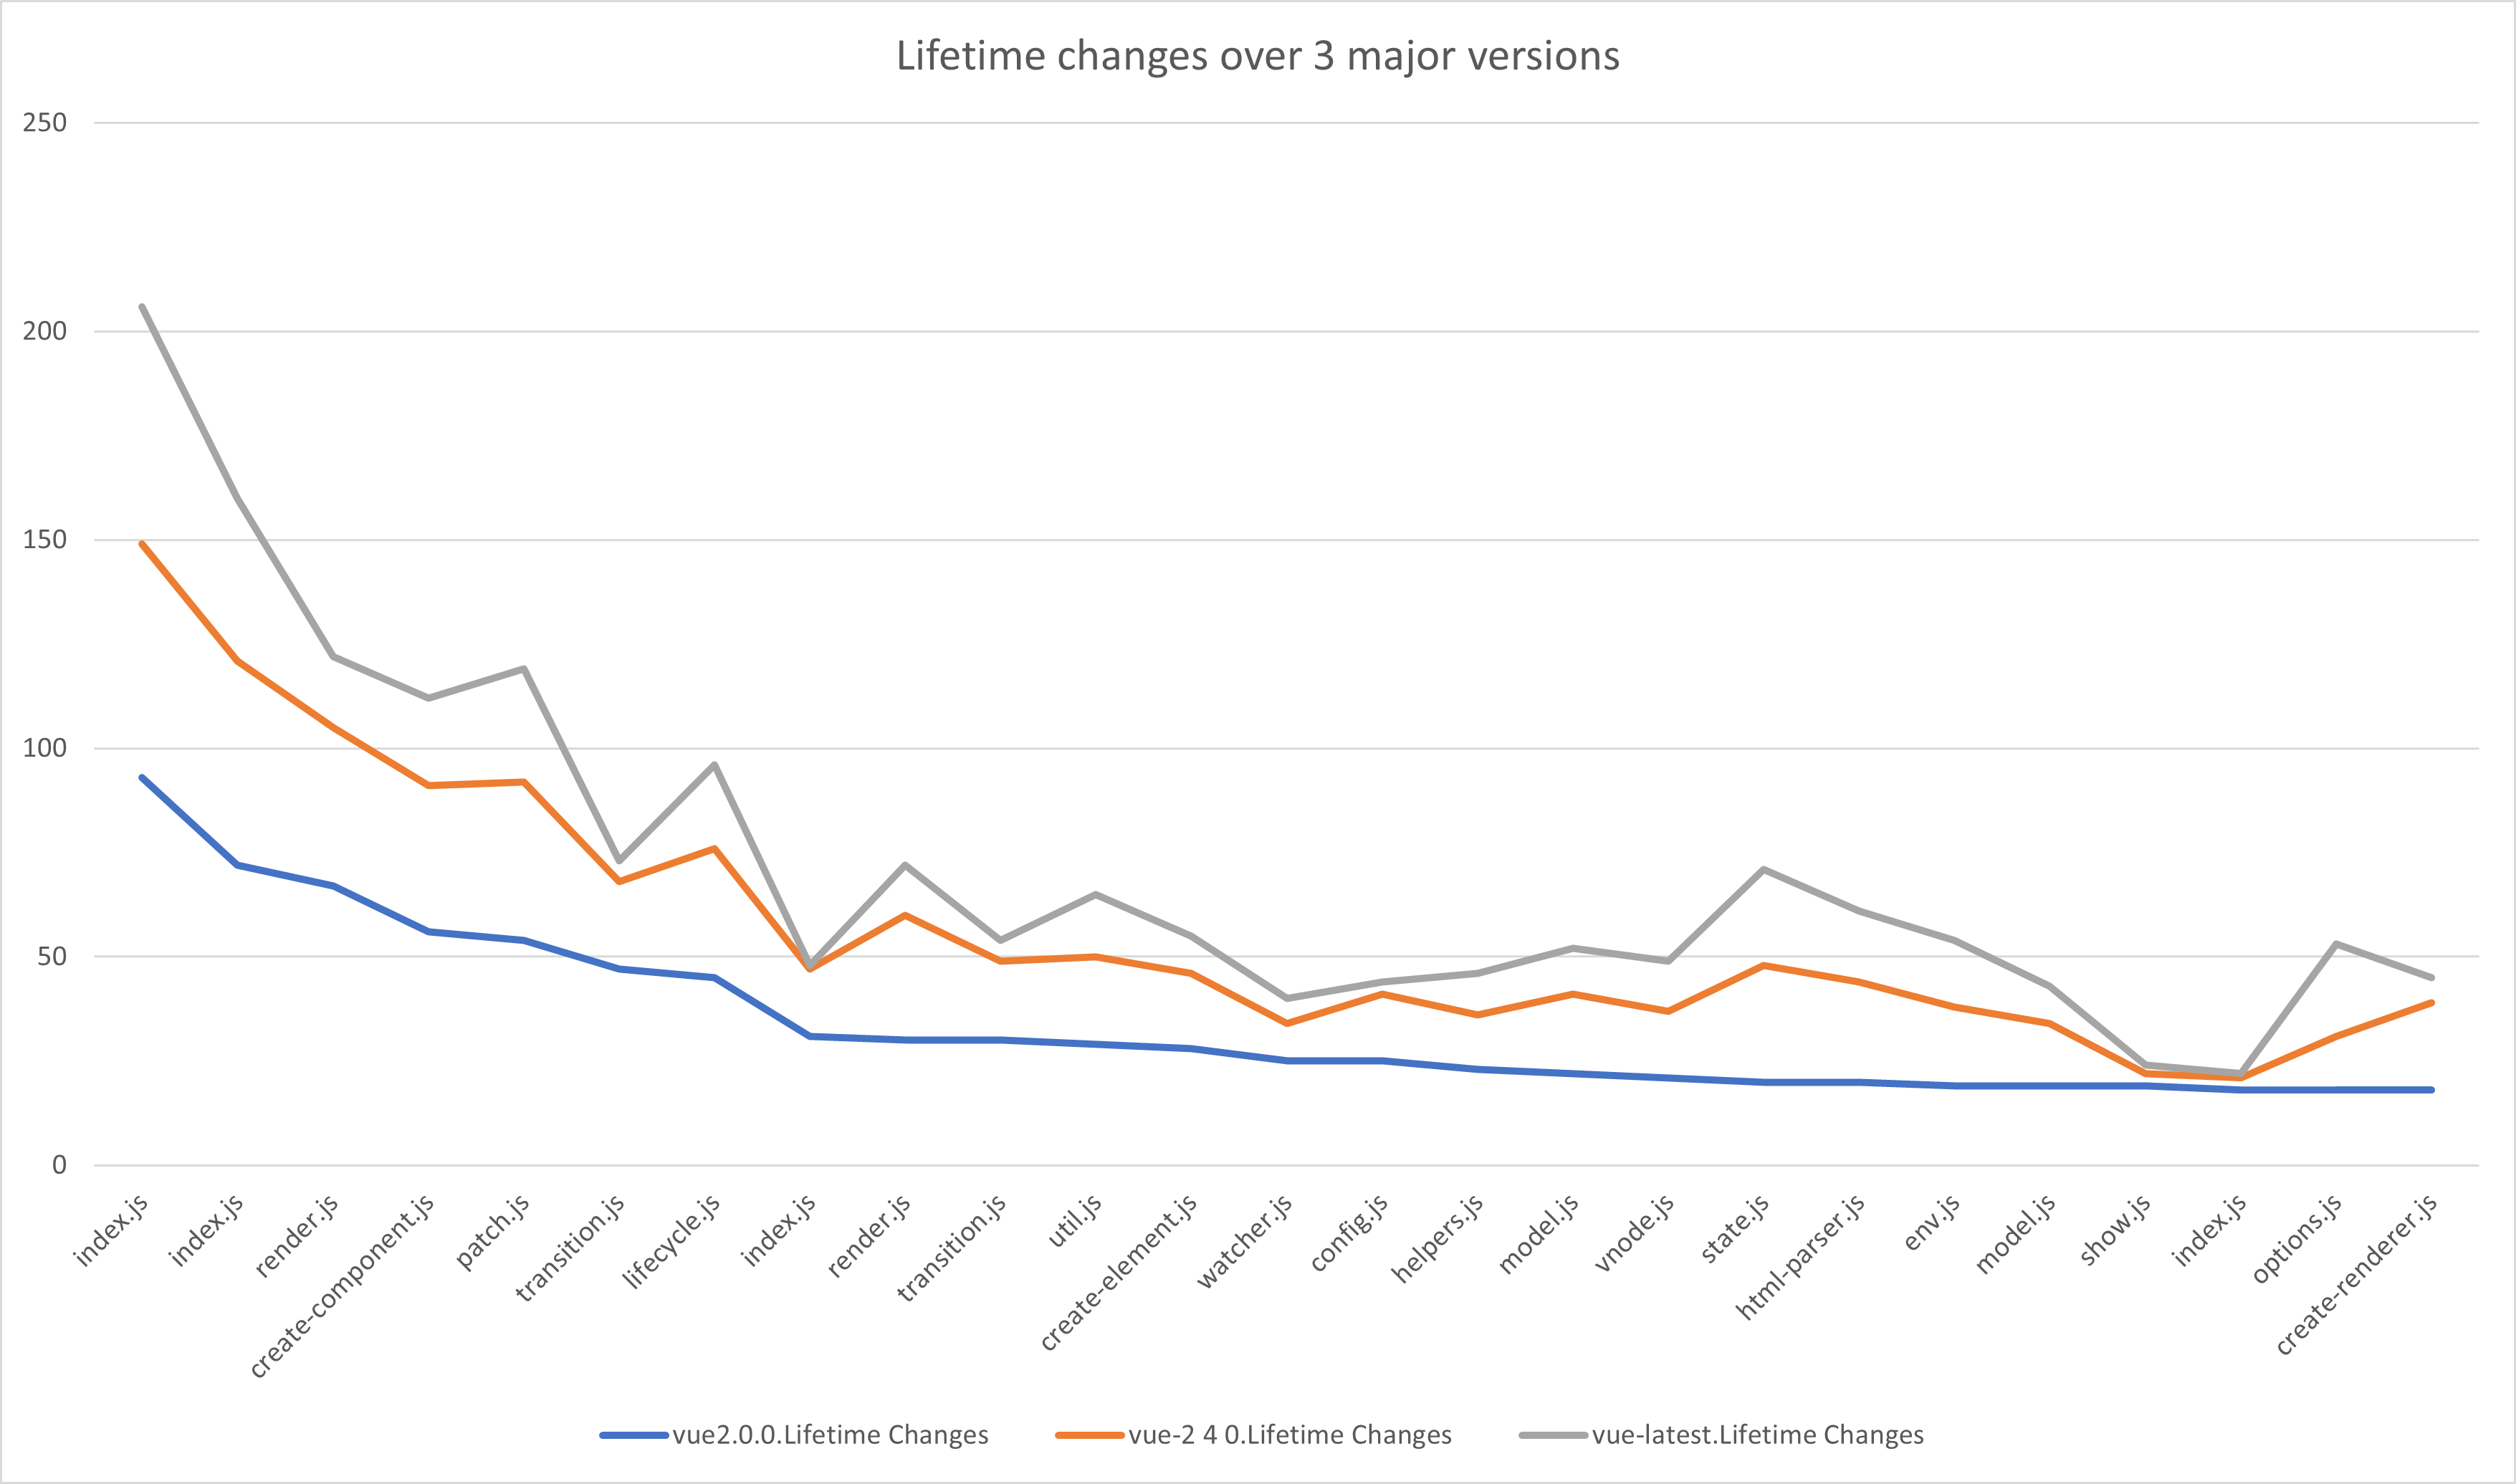
\includegraphics[width=1\textwidth]{images/vue/vue-all-lifetime-changes.png}
    \caption{A vue legtöbbet módosított fájljainak alakulása 2016 és 2020 között}
    \label{fig:vue-all-top-files}
\end{figure}

\begin{figure}[H]
    \centering
    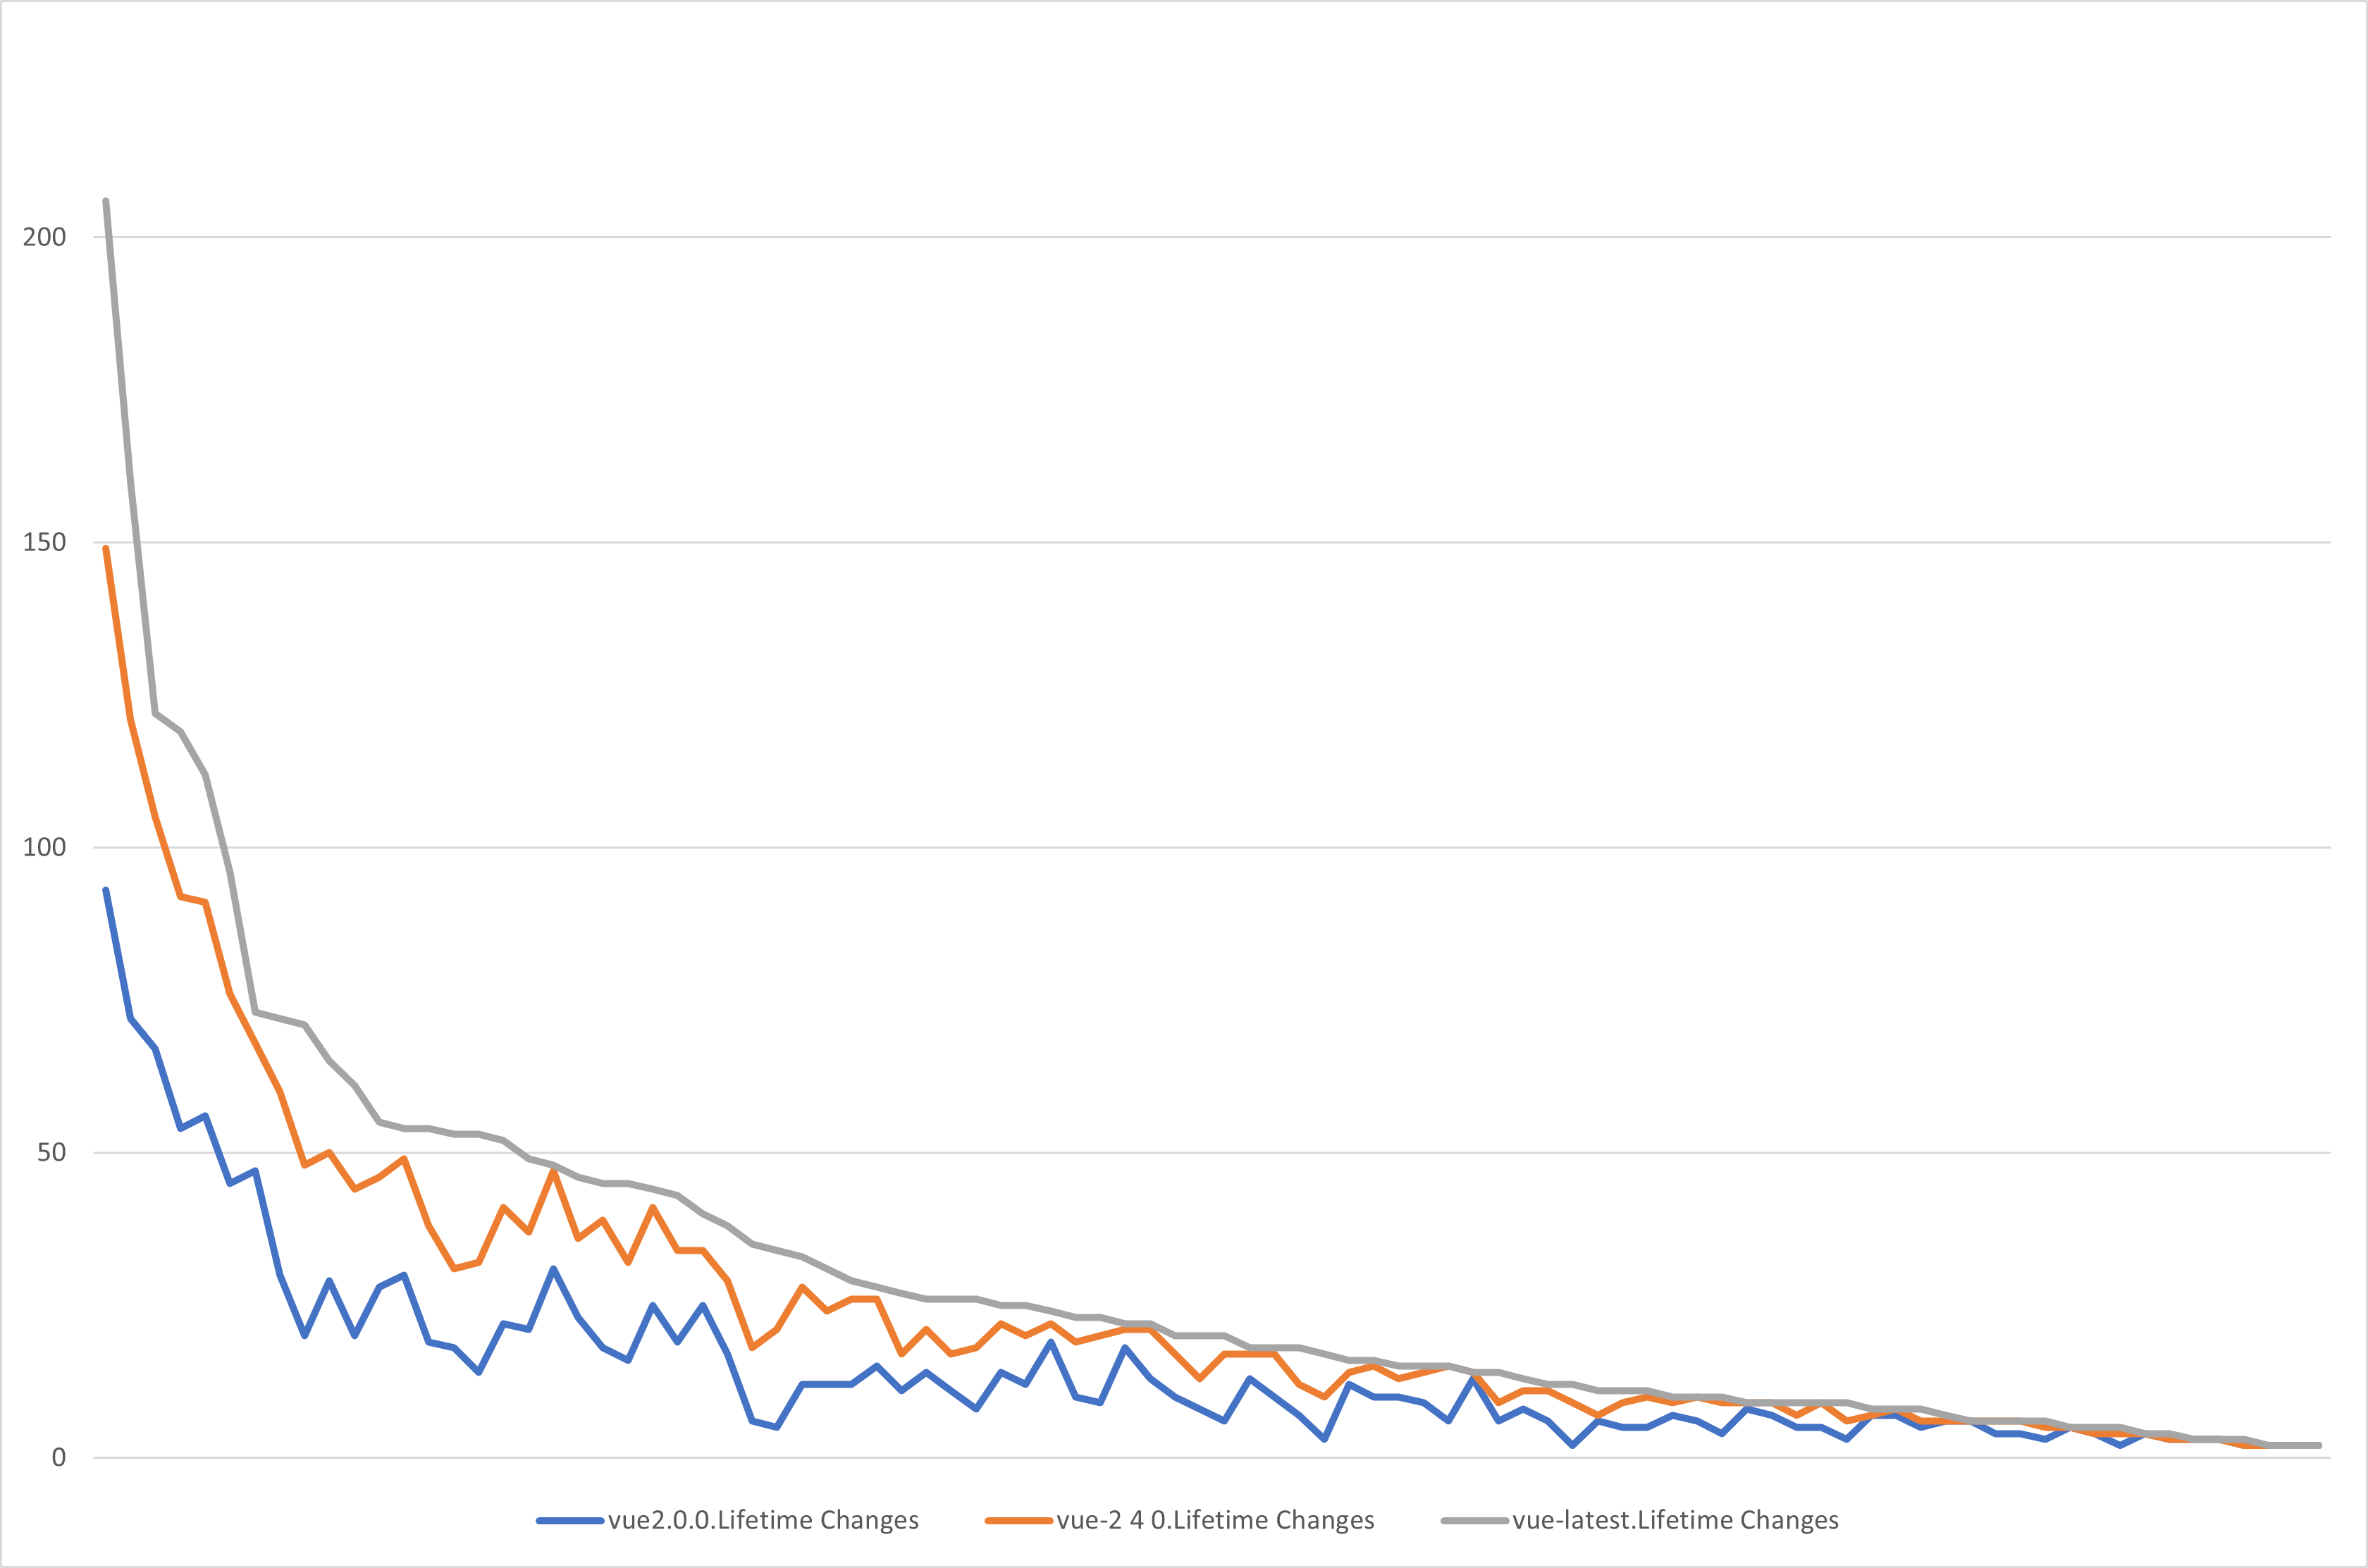
\includegraphics[width=1\textwidth]{images/vue/vue-all-lifetime-changes-comp-full.png}
    \caption{A vue projekt összes fájljának módosítási számai}
    \label{fig:vue-all-files-lifetime-changes}
\end{figure}

\begin{figure}[H]
    \centering
    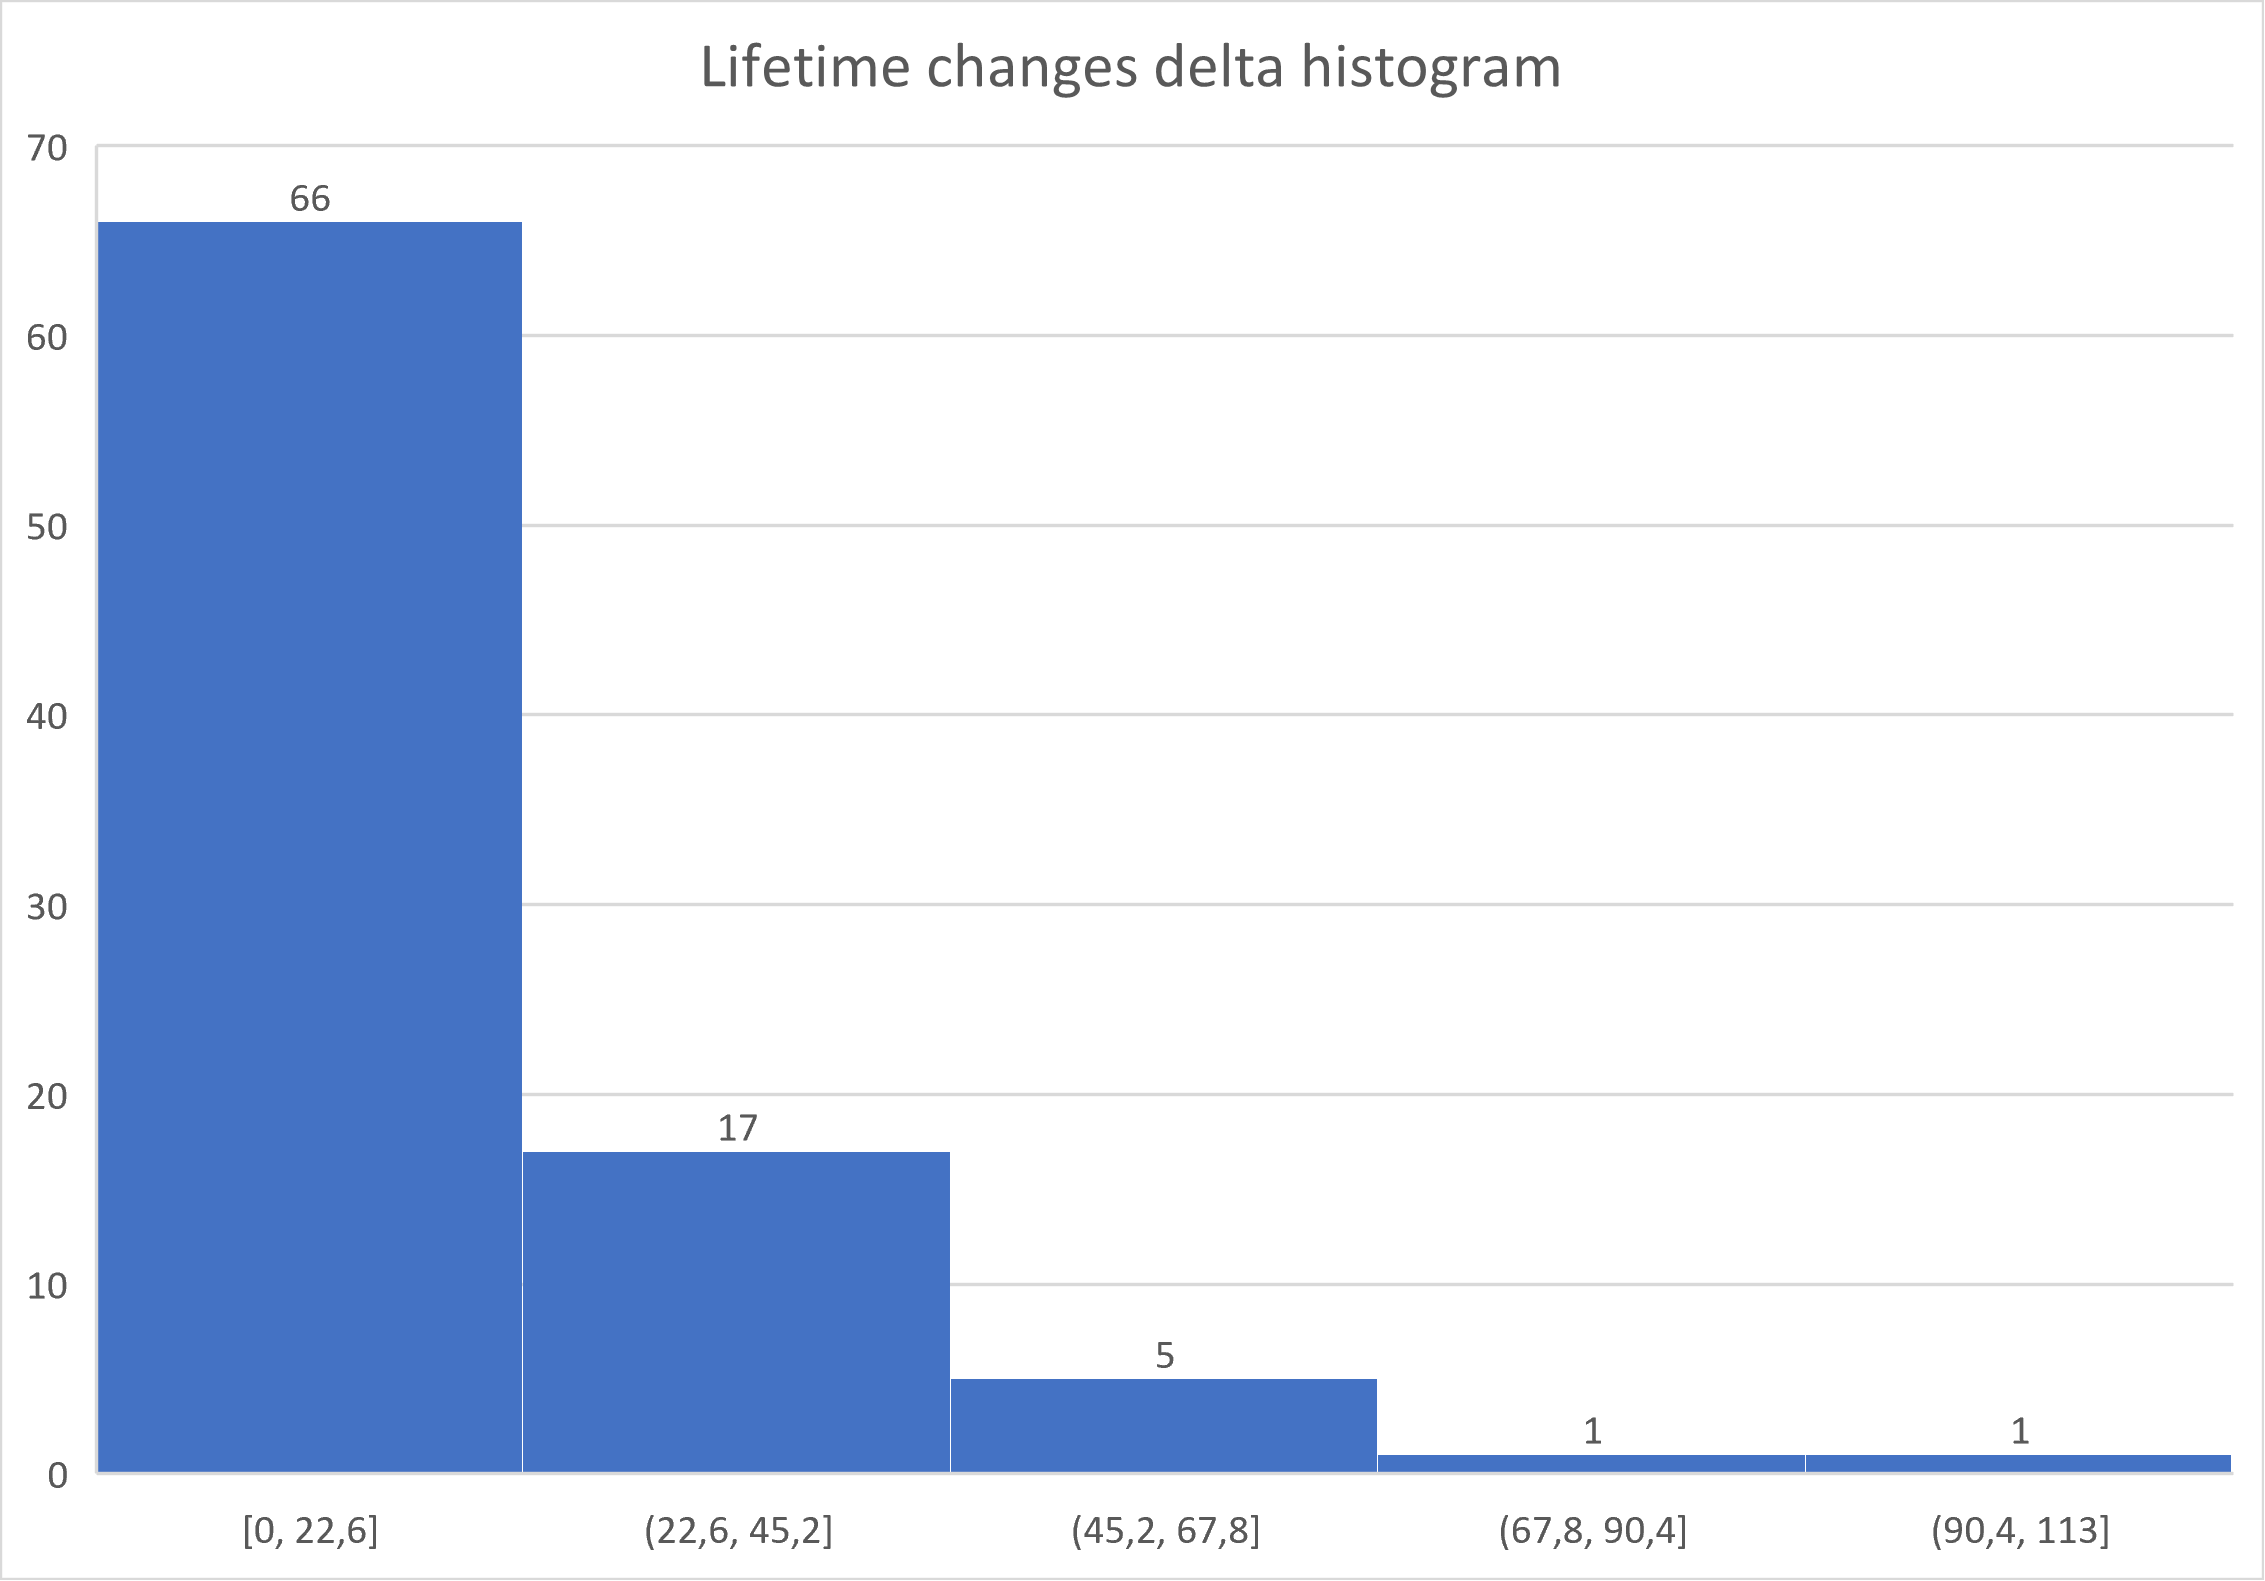
\includegraphics[width=1\textwidth]{images/vue/vue-all-lifetime-changes-delta-hist.png}
    \caption{A vue projekt 2.0-ás és legfrissebb verzióiban lévő fájlok módosítási számainak deltái}
    \label{fig:vue-all-delta-hist}
\end{figure}

\begin{figure}[H]
    \centering
    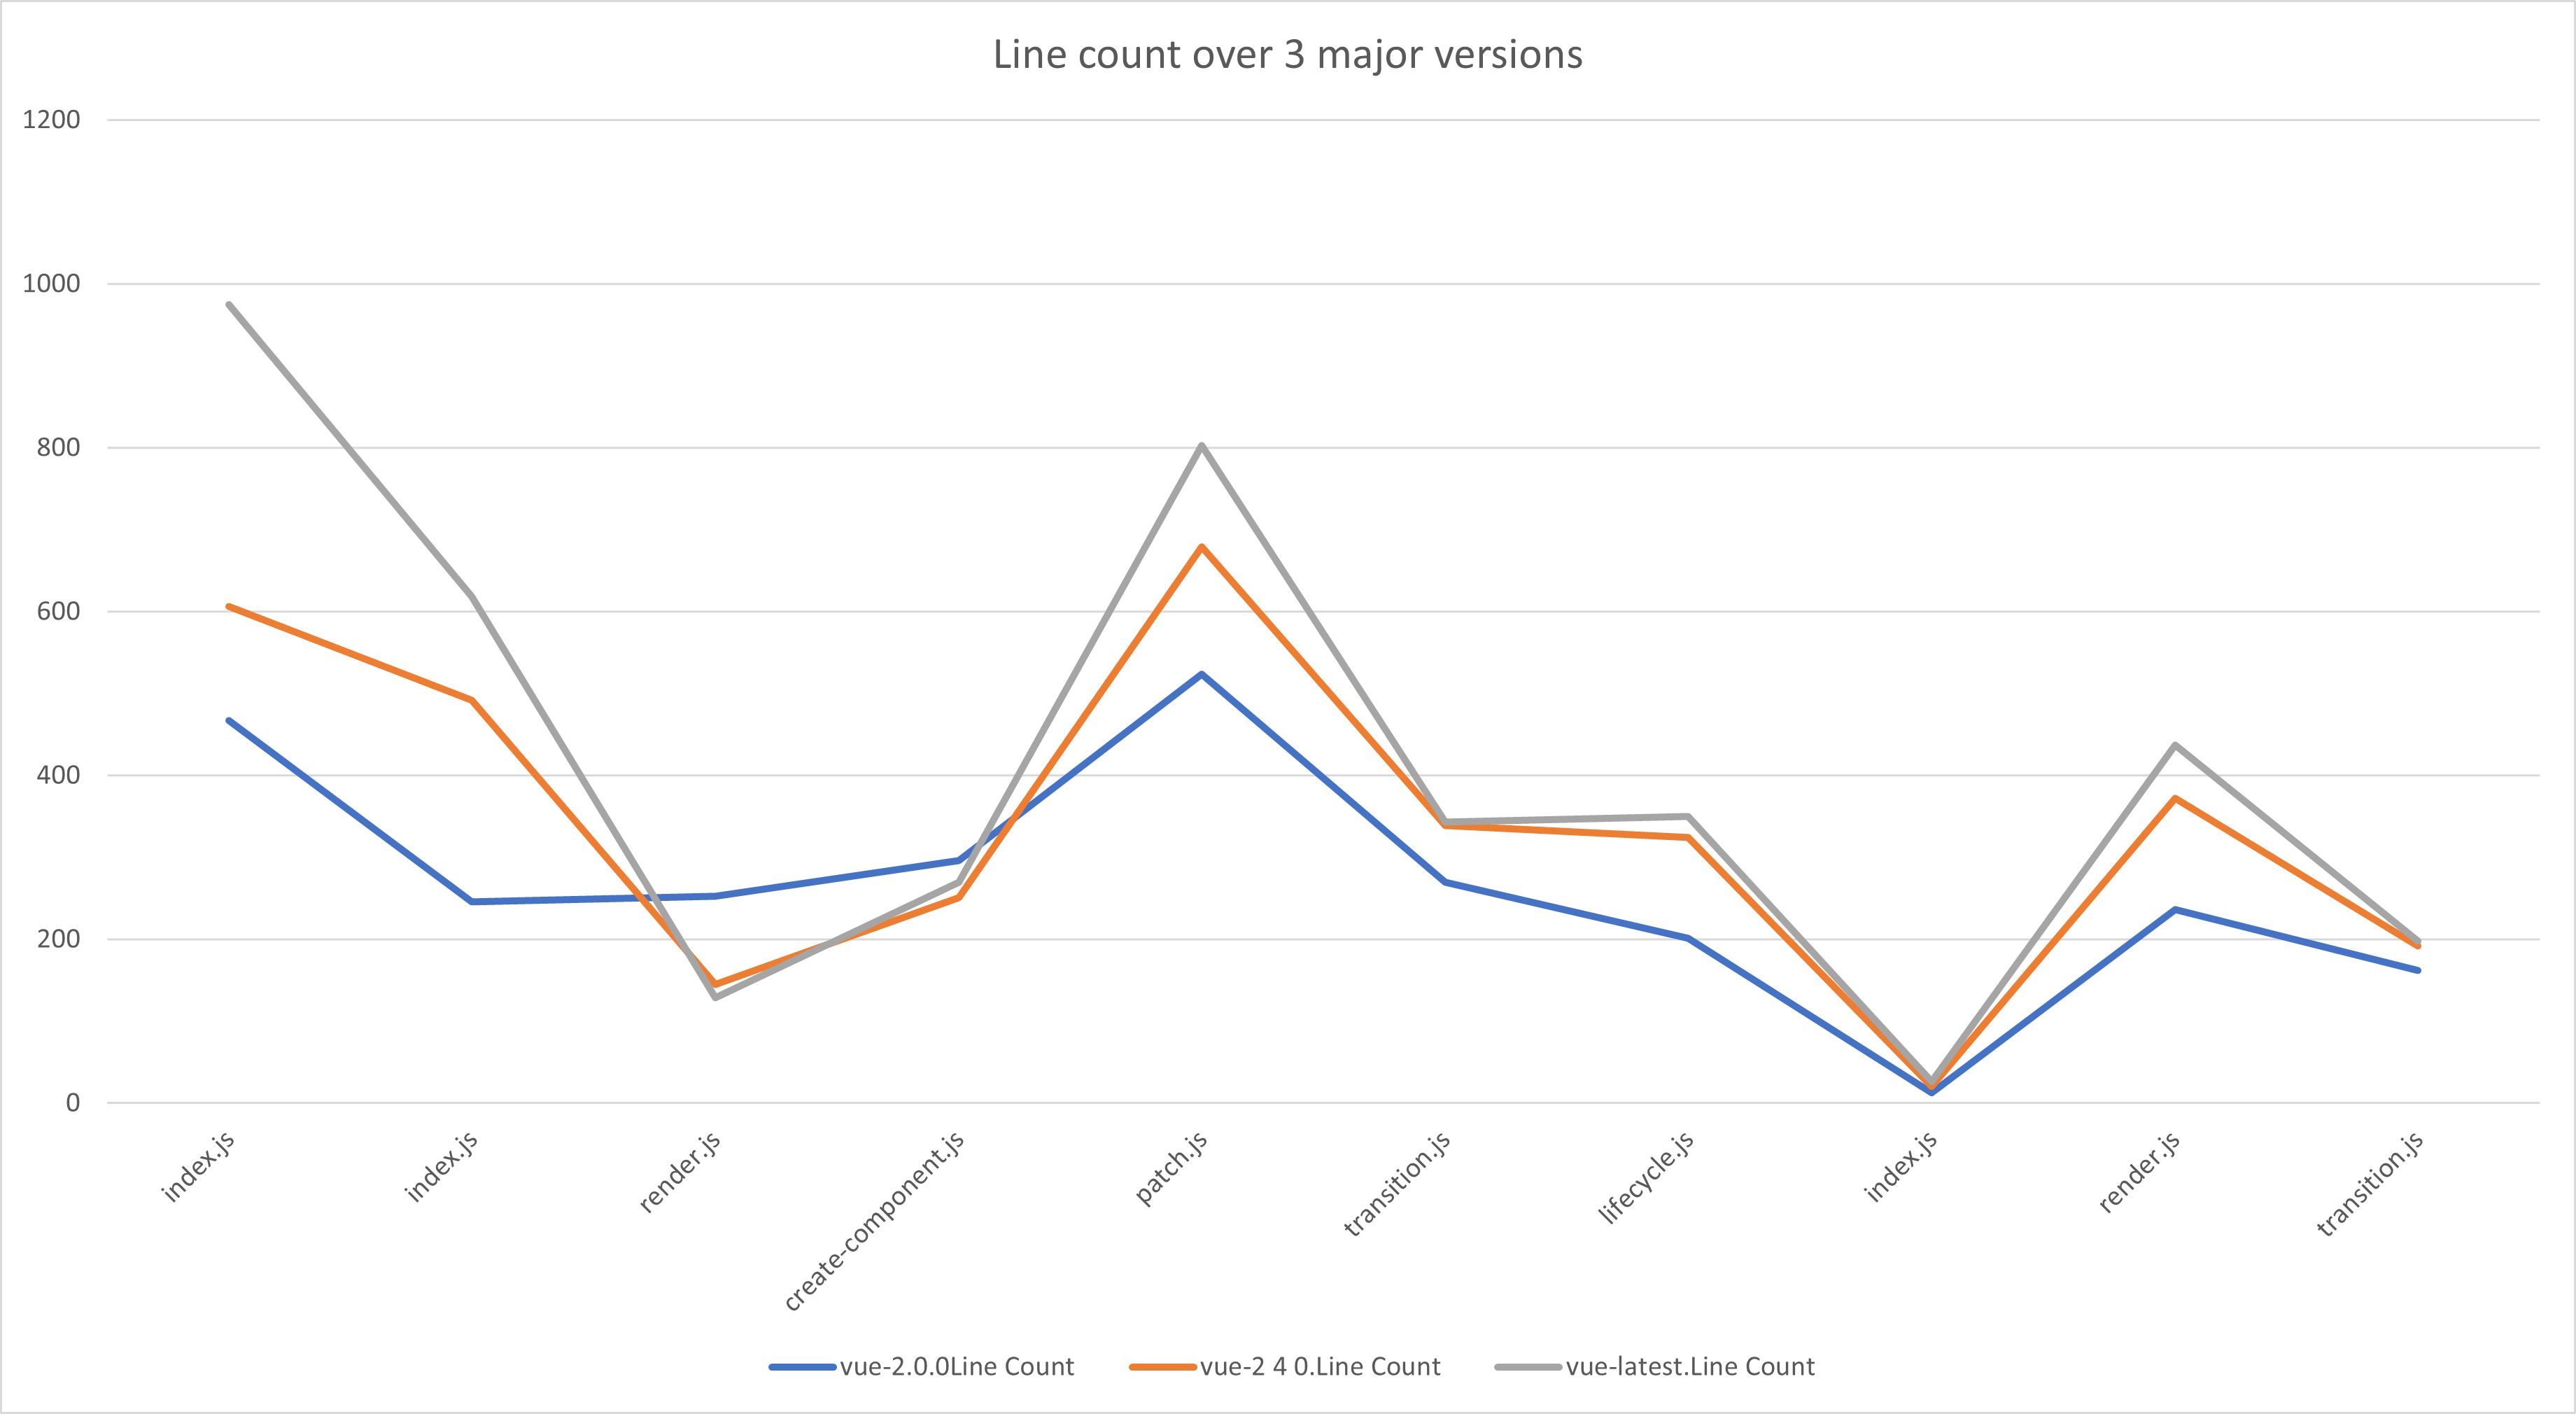
\includegraphics[width=1\textwidth]{images/vue/vue-all-line-count.png}
    \caption{A vue projektben lévő fájlok méretének változása 3 verzión keresztül}
    \label{fig:vue-all-line-count}
\end{figure}

Végül tekintsük a \ref{fig:vue-all-delta-hist} ábrát, amin a fájlok coverage-e látható. Kijelenthetjük, hogy a vue esetében a teszt coverage semmilyen moderáló hatást nem gyakorolt a változtatási gócpontokra, illetve a gócpontok növekedése nem hatott negatívan a unit tesztekre.

\begin{figure}[H]
    \centering
    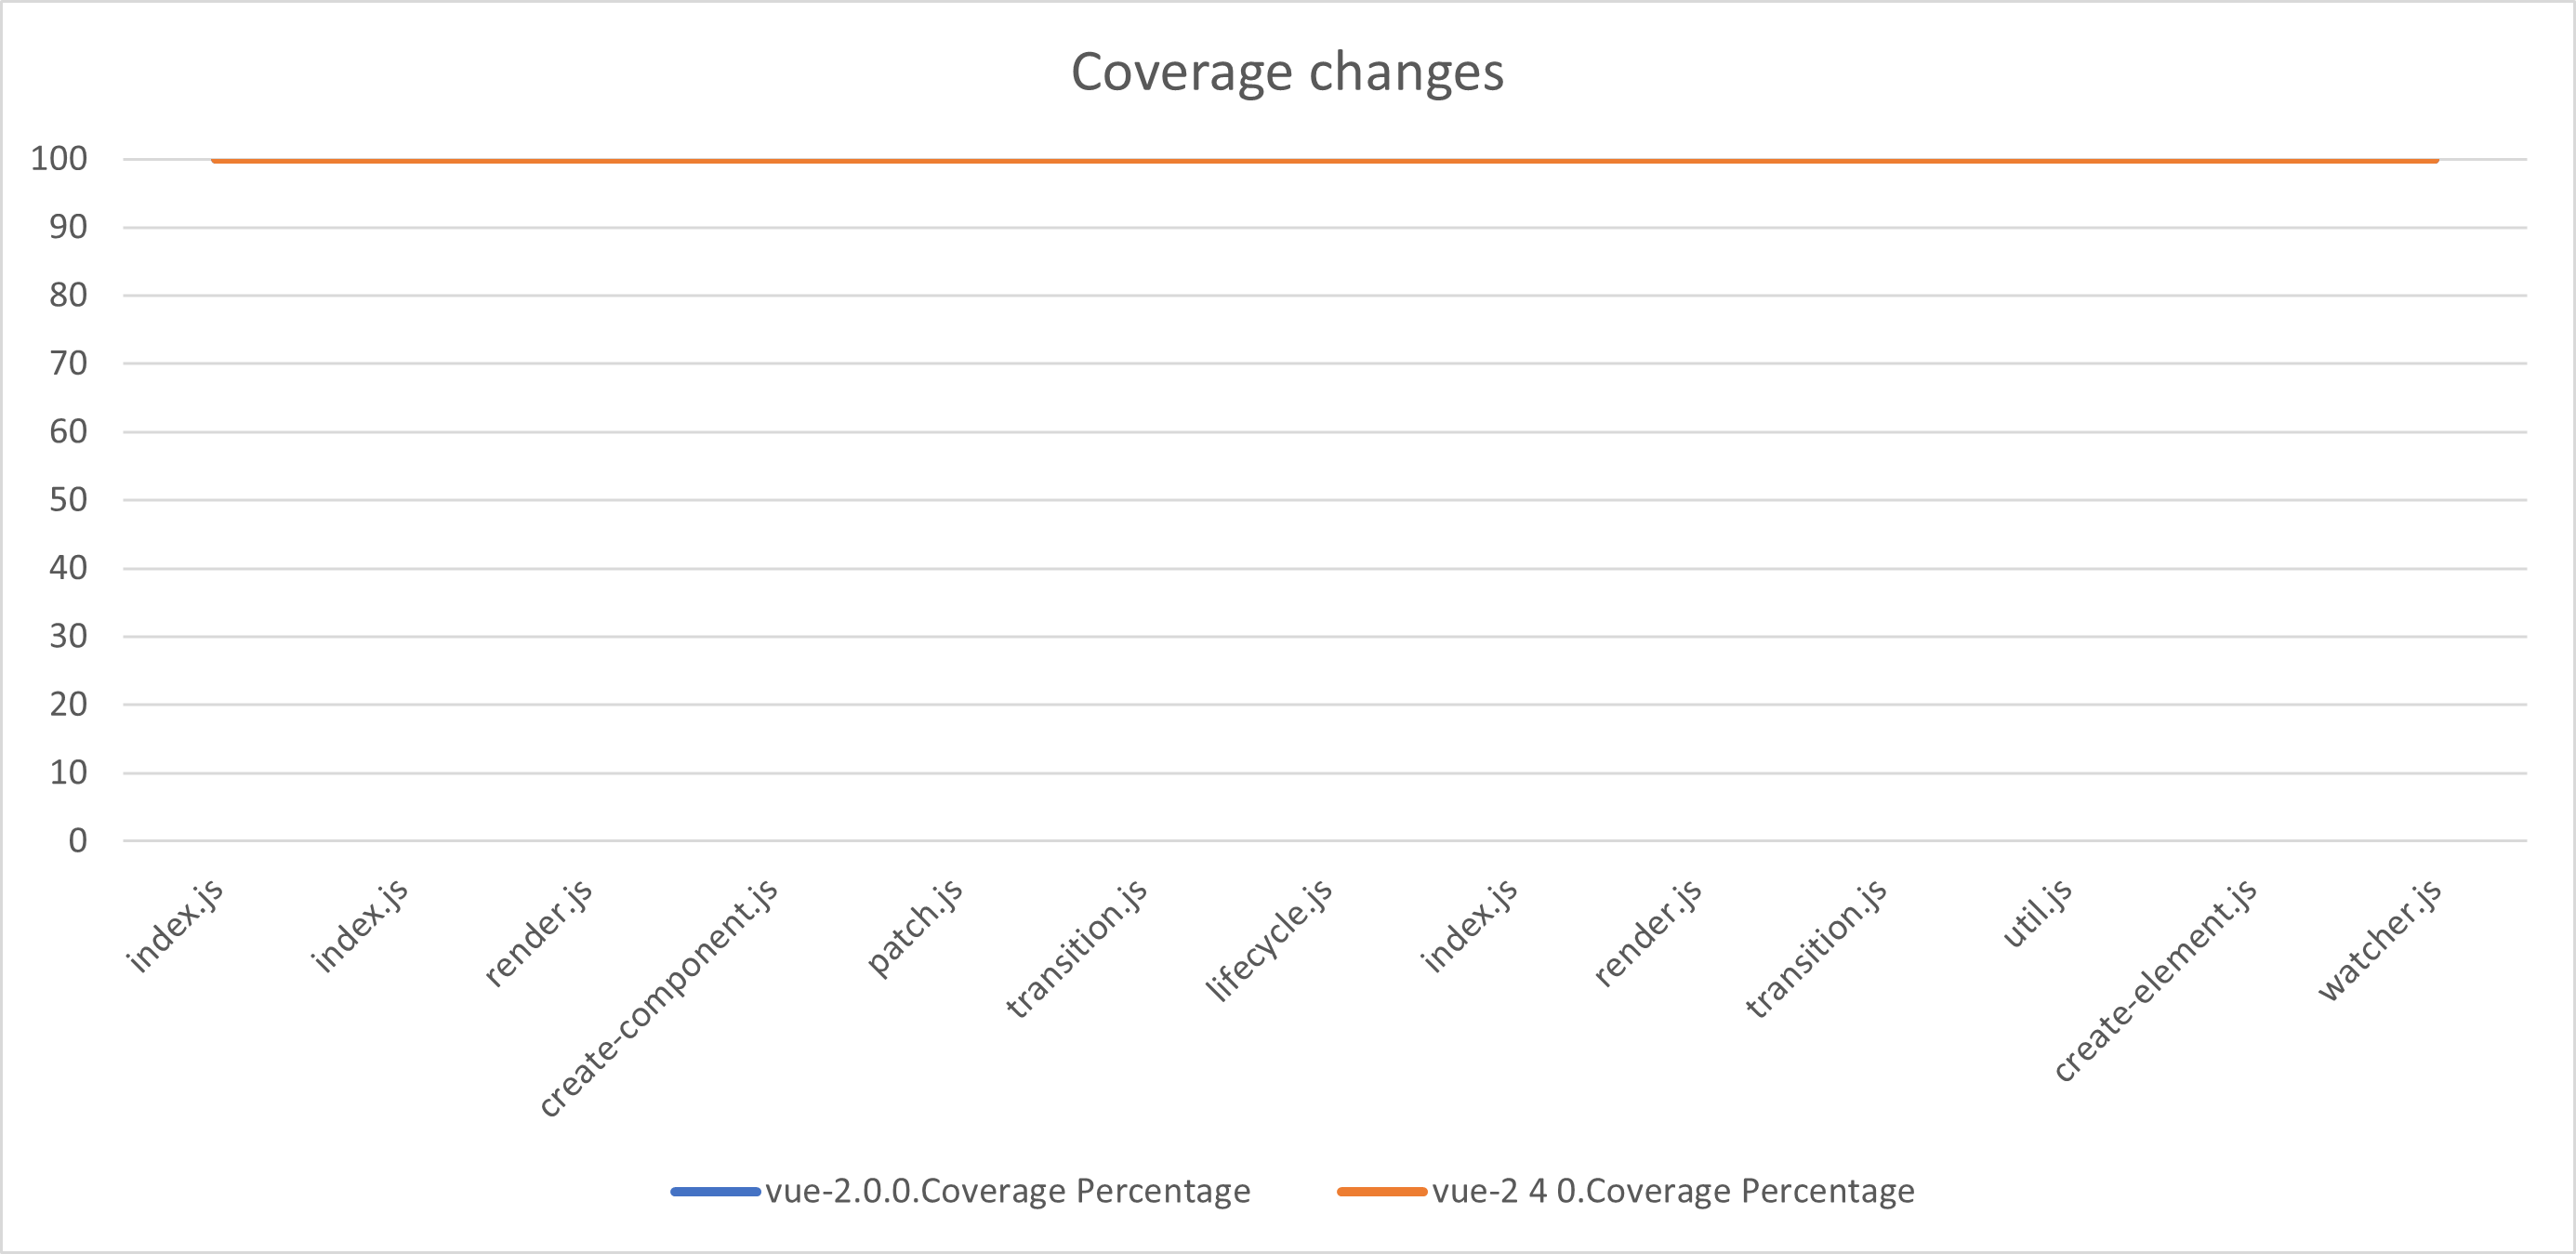
\includegraphics[width=1\textwidth]{images/vue/vue-all-coverage.png}
    \caption{A vue projekt teszt coverage-ének változása 3 verzión keresztül}
    \label{fig:vue-all-coverage}
\end{figure}

\subsection{Megfigyelések}

A vue projekt elemzése összességében sok érdekes trendet tárt fel. Láttuk például, hogy a projekt születésétől kezdve gócpontot alkotó \code{compile.js} még egy teljes refactor után is ugyanazokat a mintákat mutatta, mint korábban.

Megfigyeltük továbbá, hogy a projekt elején fennálló módosítási trendek szinte változatlanok maradnak a projekt élettartama során. Ebbe beleértendő az is, hogy új gócpontok nem igazán tudnak kialakulni, a komplexitás lokalitása változatlan marad.

Végül láttuk azt is, hogy a coverage-nek semmilyen moderáló hatása nincs ezekre a negatív trendekre, hiszen a vue projekt gócpontjai kivétel nélkül 100\%-os coverage-el rendelkeznek. Igaz viszont az is, hogy a gócpontok növekedése nem vezetett a coverage romlásához sem.


\section{Moment.js}

A második mélyebben megvizsgált kódbázis a moment.js\footnote{https://momentjs.com/} lesz. A moment éveken át volt a de facto JavaScript-ben írt dátum-idő könyvtár, azonban 2020-ban különböző okoknál fogva a fejlesztése befejeződött.

A moment kódbázisa két szempontból lesz érdekes: egyrészt "késznek" tekinthető, másrészt egy nagyon jól definiált, kis problémát volt hivatott megoldani a kezdetekből.

Ideális esetben a legelső kiadástól lenne érdemes kezdeni az analízist, azonban a moment 1.0 megjelenésekor sem unit tesztek, sem coverage report nem voltak a projekthez, ráadásul a kódbázis egy masszív JavaScript fájl volt. A moment 2.0 megjelenése azonban viszonylag közel van az 1.0-hoz és a 2.10.5-ös minor release-től kezdve elérhető a coverage report, úgyhogy az lesz a kezdőpont

A \ref{fig:moment-2.10.1-changes} ábrán látható az összes fájl módosítási száma és a fájlokhoz tartozó egyedi szerzők száma. Egy érdekes dolog már most megfigyelhető: ellentétben a vue-val, itt a szórás a különböző fájlok módosítási számai között viszonylag alacsony. Ehhez viszont hozzátartozik a korábban említett 1.0-ás kiadás, ahol a kódbázis egy \code{moment.js} nevű fájl volt, aminek a története egy újraírás miatt nem jelenik meg a 2.x-es kiadásokban.

\begin{figure}[H]
    \centering
    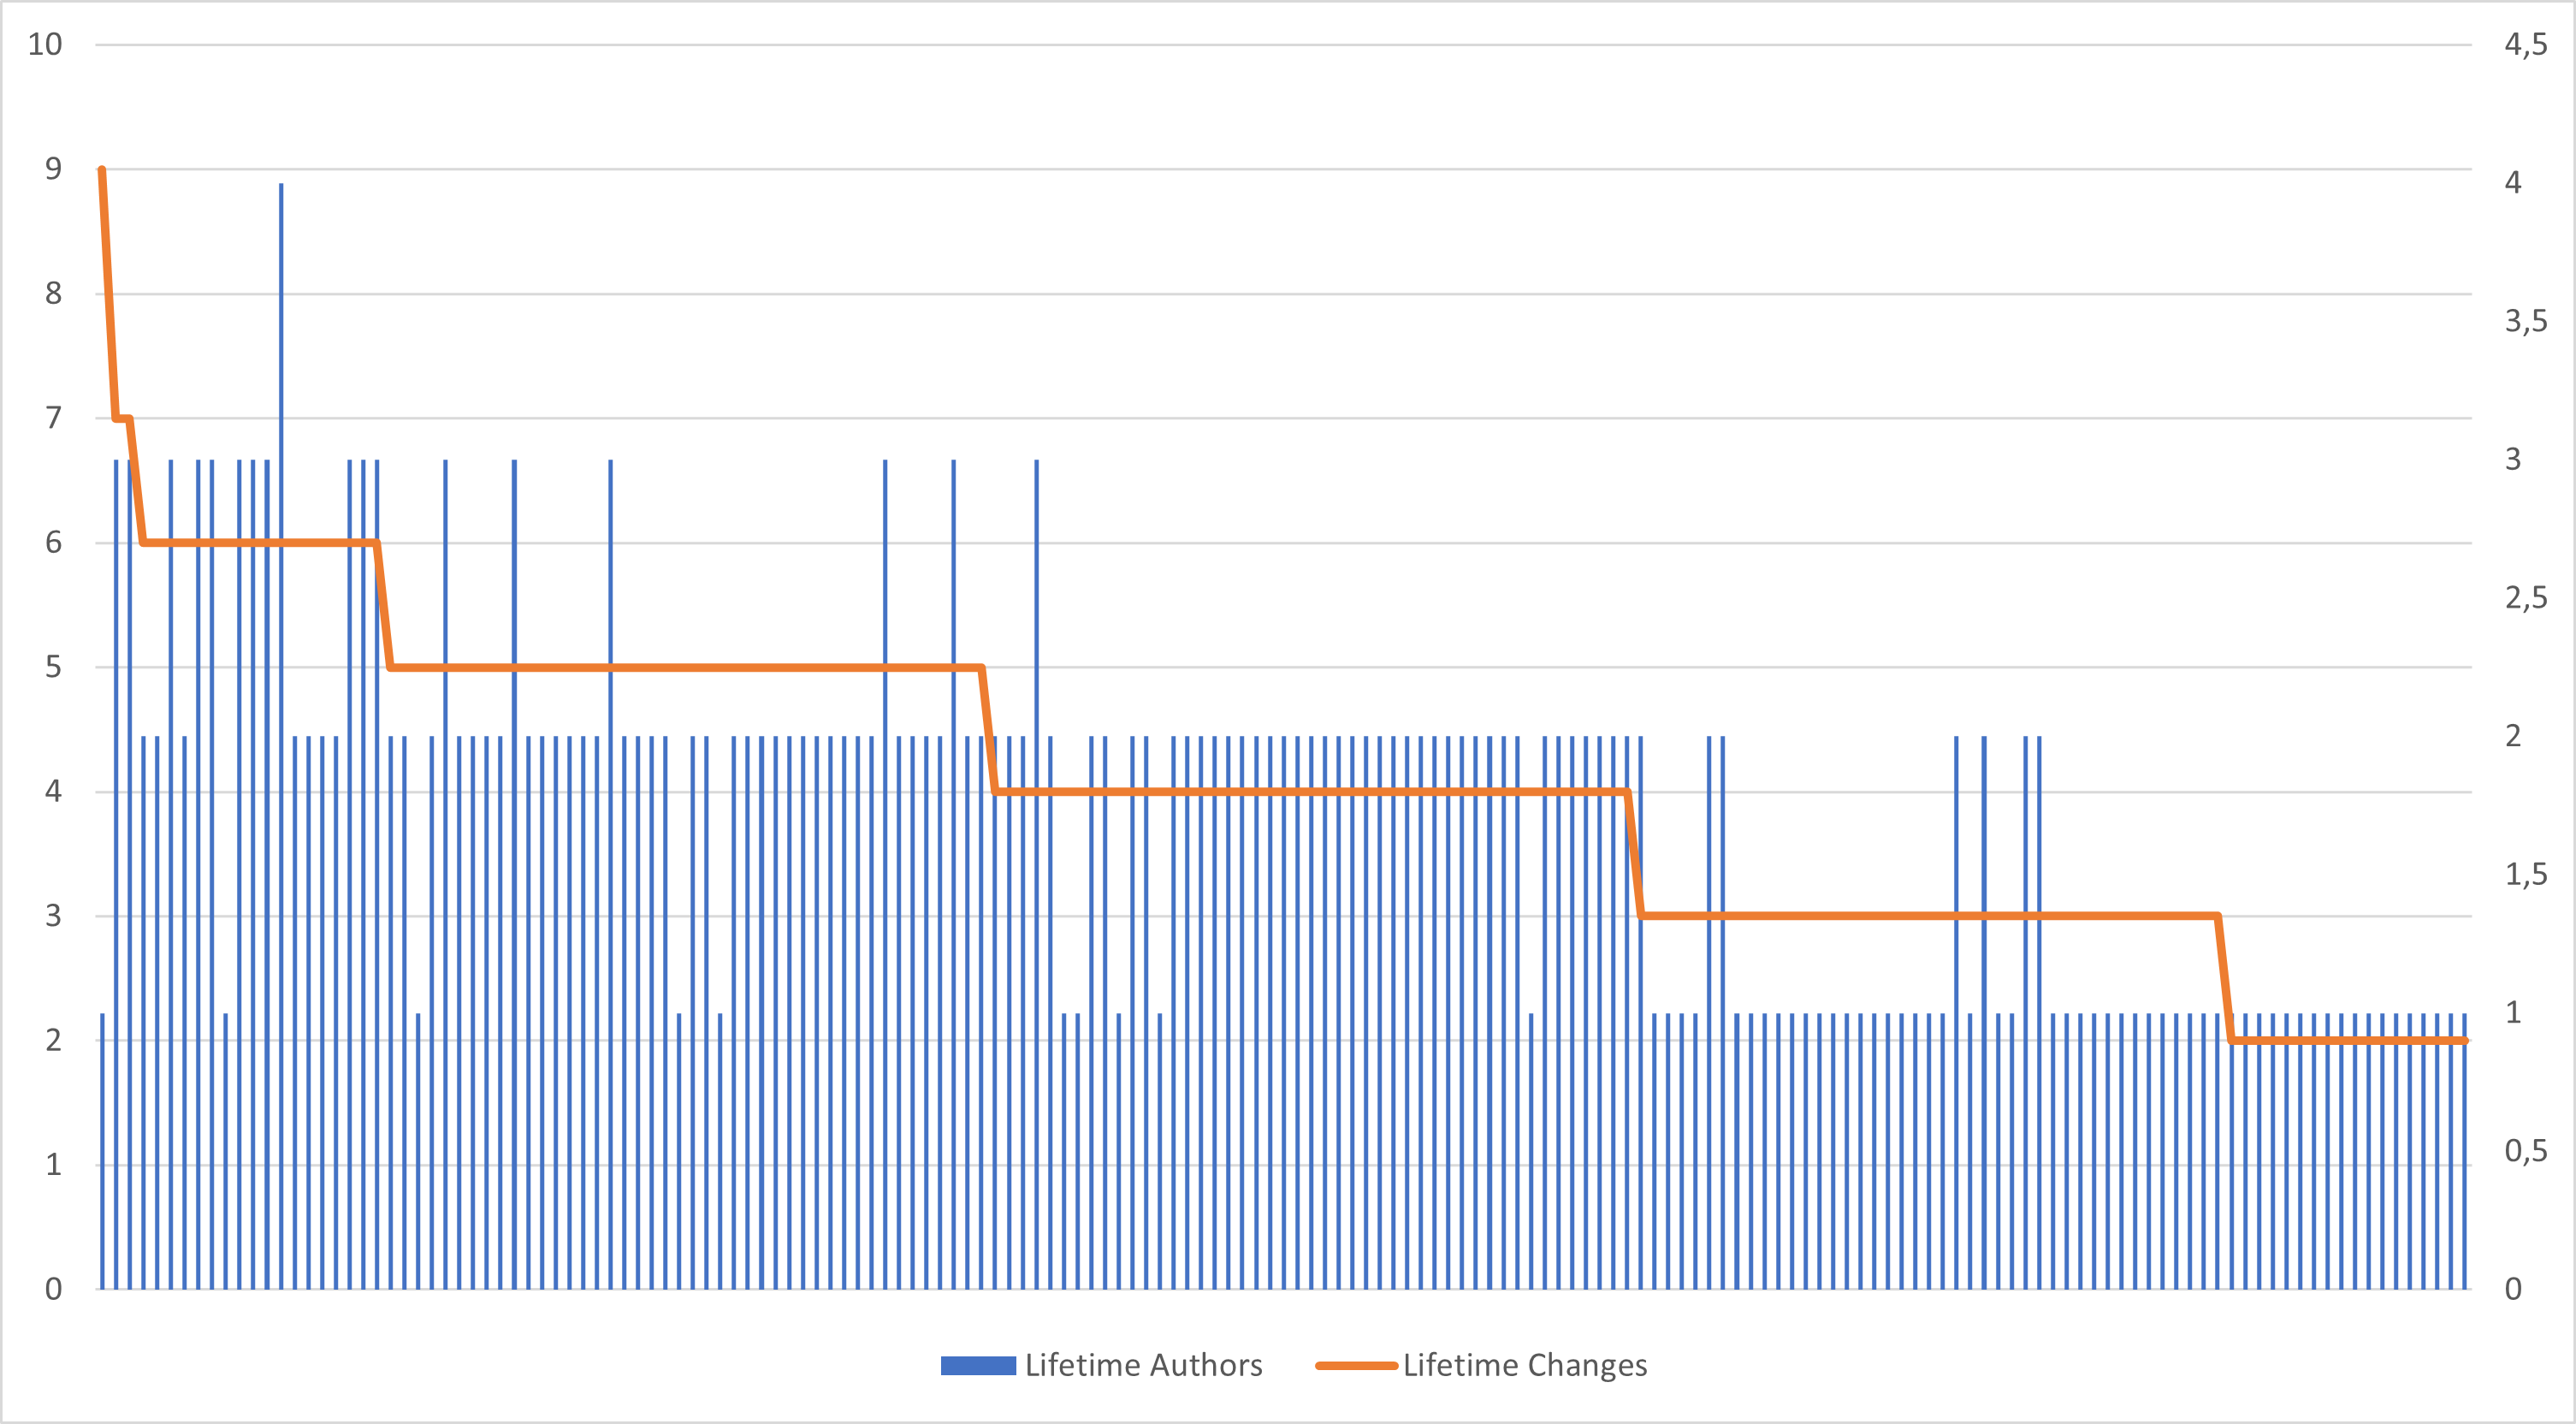
\includegraphics[width=1\textwidth]{images/moment/moment-2.10.5-changes.png}
    \caption{Moment.js 2.10.5-ös kiadásában lévő fájlok módosítási számai}
    \label{fig:moment-2.10.1-changes}
\end{figure}

A \ref{fig:moment-2.10.1-hist} ábrán látható hisztogram jól demonstrálja a kódbázis állapotát a 2.10.5-ös kiadásban. Ugyan technikailag itt is látható az a trend, hogy a fájlok túlnyomó többsége módosítások számát tekintve az alsó 40\%-ban van, azonban itt ez csalóka, hiszen az módosítások számának intervalluma csak 1-től 9-ig terjed.

Egyelőre kijelenthetjük, hogy a moment kódbázisa ezen a ponton kifejezetten lapos a módosítási számok tekintetében, ami ha közelebbről megnézzük a kódbázist akkor érthető is: a logika nagy része a \code{moment.js} fájlban él, különböző kisebb segéd osztályokkal, mint a \code{from-anything.js}, végezetül pedig viszonylag ritkán változtatott lokalizációs fájlokban vannak definiálva a különböző dátum formátumok.

\begin{table}[h]
    \centering
    \begin{tabular}{l|l|l|l|l}
        Filename         & Lifetime Authors & Lifetime Changes & Line \# & Coverage \%       \\ \hline
        moment.js        & 1                & 9                & 68      & 98.02224969097651 \\
        lv.js            & 3                & 7                & 87      & 100               \\
        pt-br.js         & 3                & 7                & 51      & 100               \\
        from-anything.js & 2                & 6                & 96      & 0                 \\
        sl.js            & 2                & 6                & 150     & 90.1639344262295  \\
        day-of-week.js   & 3                & 6                & 134     & 0                 \\
        my.js            & 2                & 6                & 84      & 100               \\
        hu.js            & 3                & 6                & 100     & 92.85714285714286 \\
        hr.js            & 3                & 6                & 131     & 89.1304347826087  \\
        prototype.js     & 1                & 6                & 145     & 0
    \end{tabular}
    \caption{Moment.js 2.10.5}
    \label{tab:moment-2105}
\end{table}

\begin{figure}[H]
    \centering
    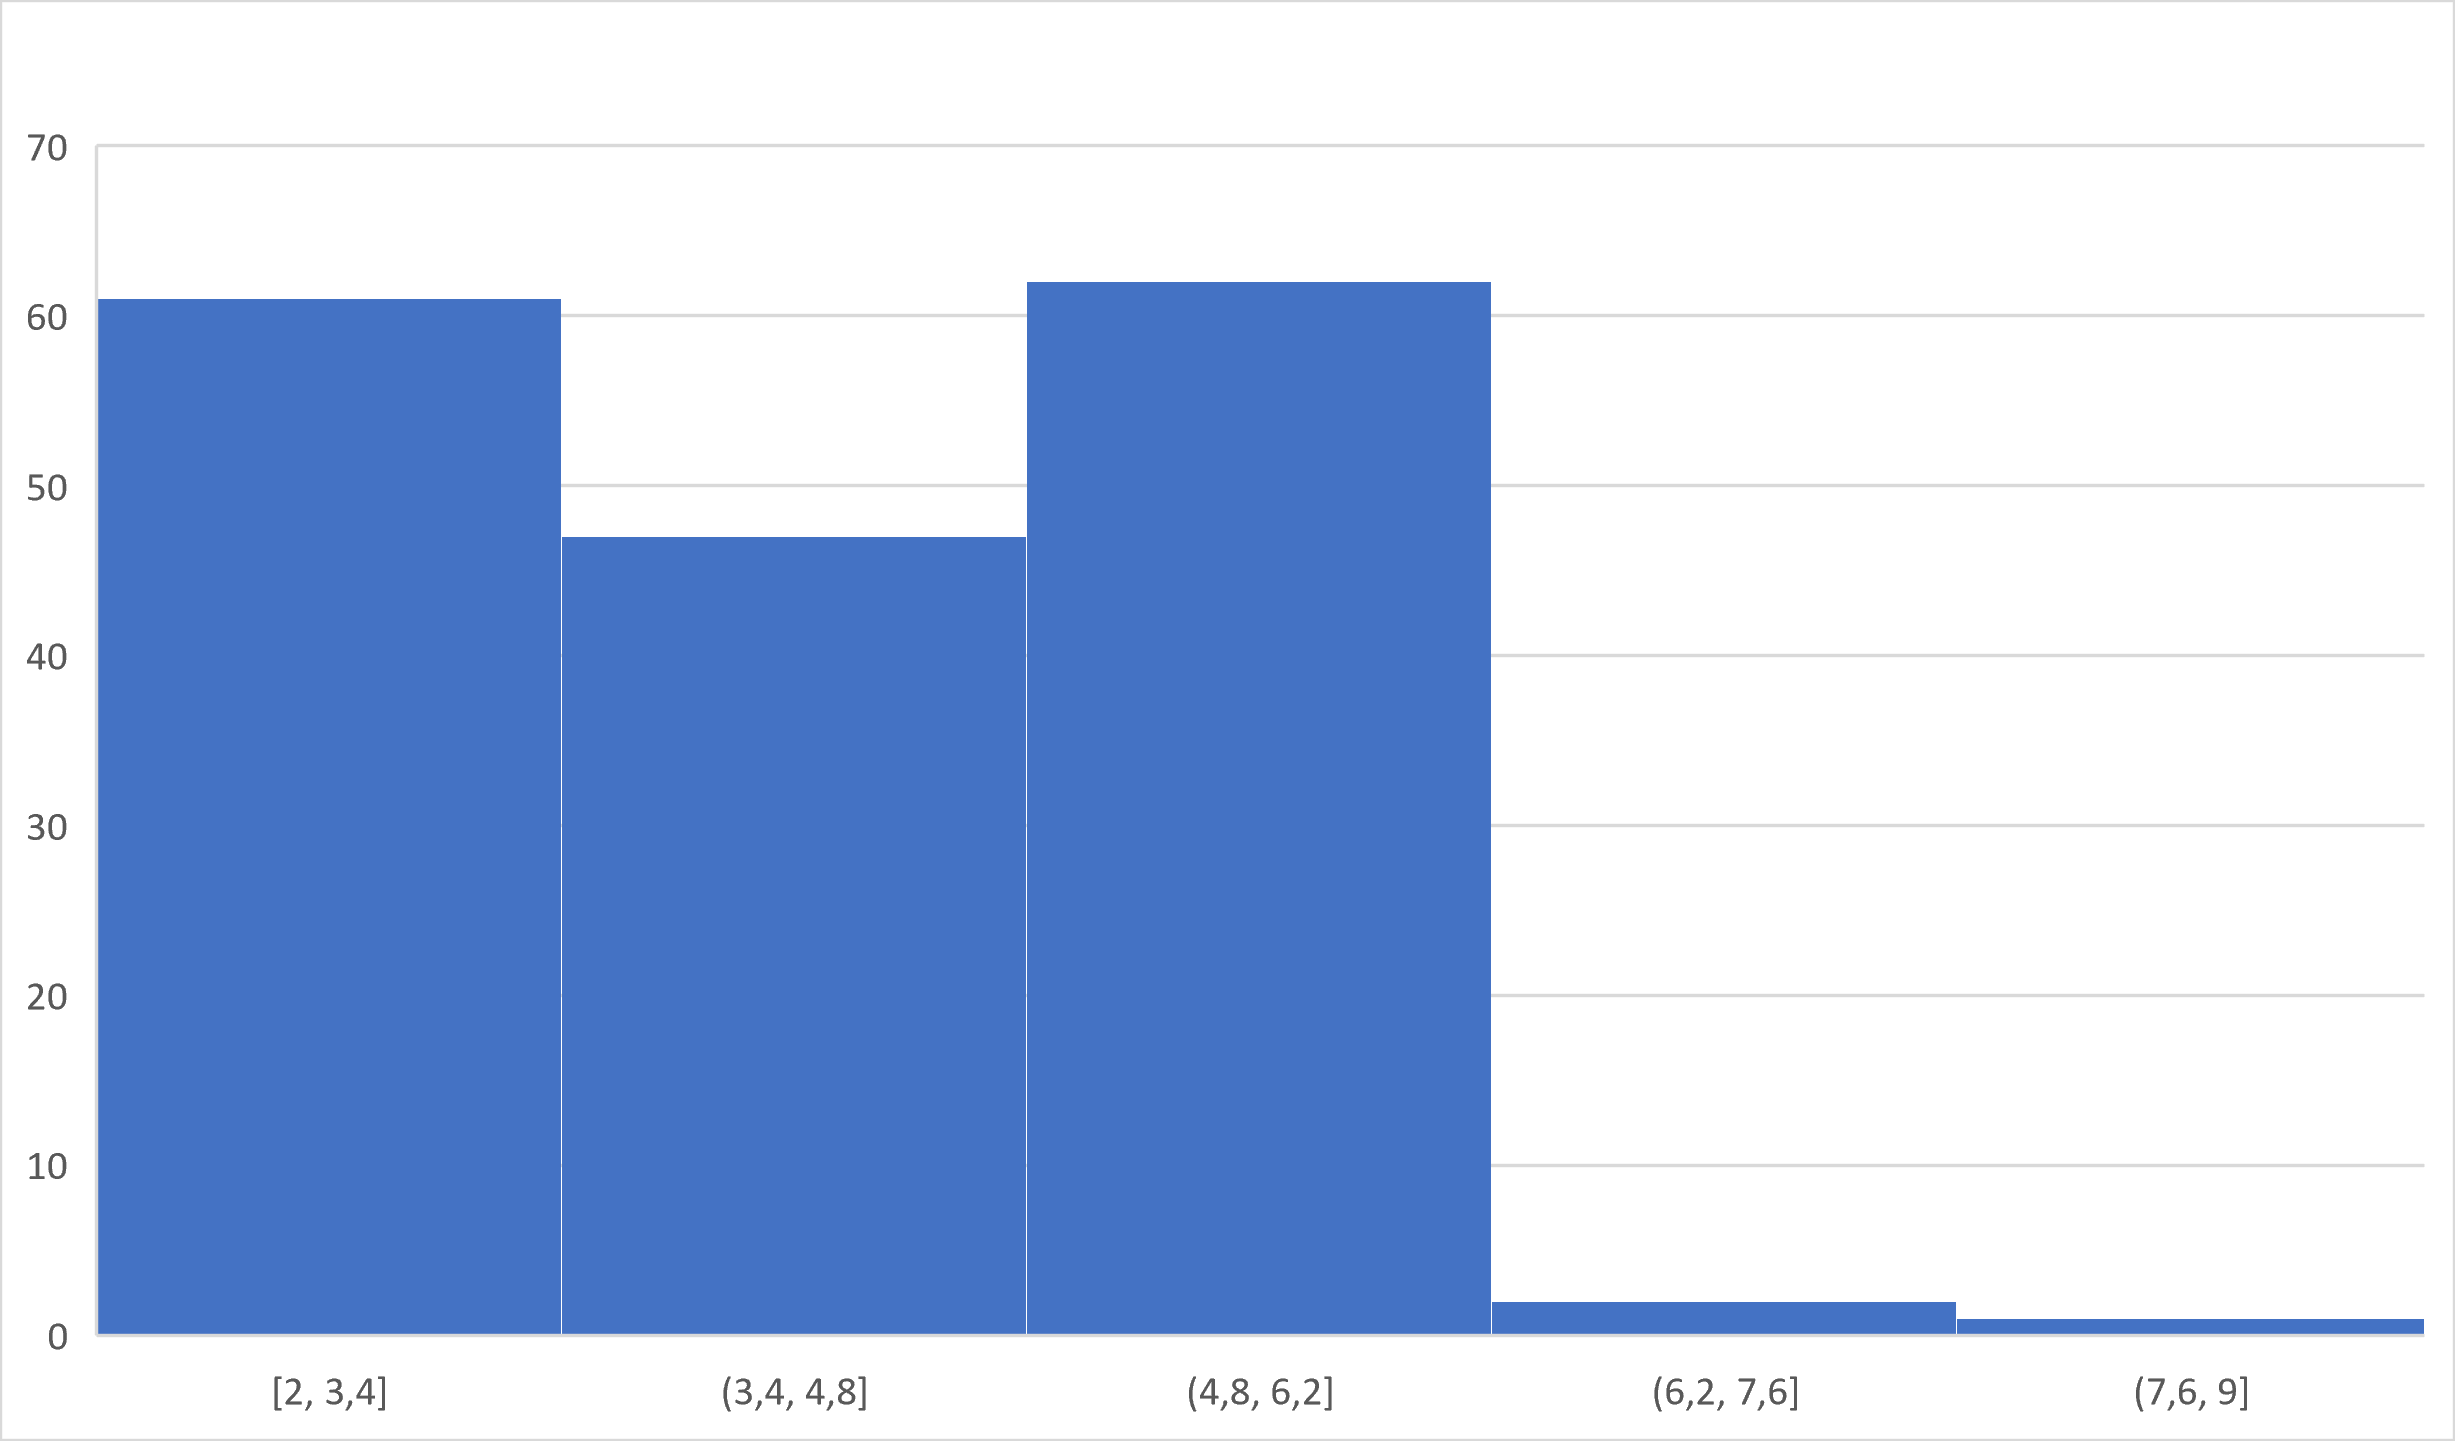
\includegraphics[width=1\textwidth]{images/moment/moment-2.10.5-hist.png}
    \caption{Moment.js 2.10.5-ös kiadásában lévő fájlok módosítási számainak hisztogramja}
    \label{fig:moment-2.10.1-hist}
\end{figure}

Ugorjunk az időben a 2.20.1-es verzióhoz tartozó snapshot-ra, aminek a részletei a \ref{tab:moment-2.20.1} táblázatban láthatóak. Az ebből készített \ref{fig:moment-2.20.1-changes} ábra már jobban hasonlít a vue-nál látottakhoz: változtatások számának tekintetében polarizálódtak a fájlok néhány módosítási gócpont köré. A korábban már látott \code{moment.js} lett az egyik gócpont, illetve kiemelendő még a \code{from-string.js} segéd osztály. A \ref{fig:fig:moment-2.20.1-hist} ábrán is az látszik, hogy közelebb került a moment kódbázisa a korábban látottakhoz.

\begin{table}[h]
    \centering
    \begin{tabular}{l|l|l|l|l}
        Filename       & Lifetime Authors & Lifetime Changes & Line \# & Coverage \%       \\
        from-string.js & 9                & 41               & 230     & 0                 \\
        moment.js      & 9                & 40               & 95      & 96.01510067114094 \\
        month.js       & 11               & 29               & 290     & 59.63855421686747 \\
        locales.js     & 10               & 29               & 186     & 0                 \\
        ru.js          & 9                & 19               & 175     & 90                \\
        day-of-week.js & 7                & 19               & 364     & 0                 \\
        es.js          & 9                & 19               & 83      & 100               \\
        prototype.js   & 7                & 17               & 150     & 50                \\
        from-array.js  & 7                & 16               & 147     & 0
    \end{tabular}
    \caption{Moment.js 2.20.1}
    \label{tab:moment-2.20.1}
\end{table}

\begin{figure}[H]
    \centering
    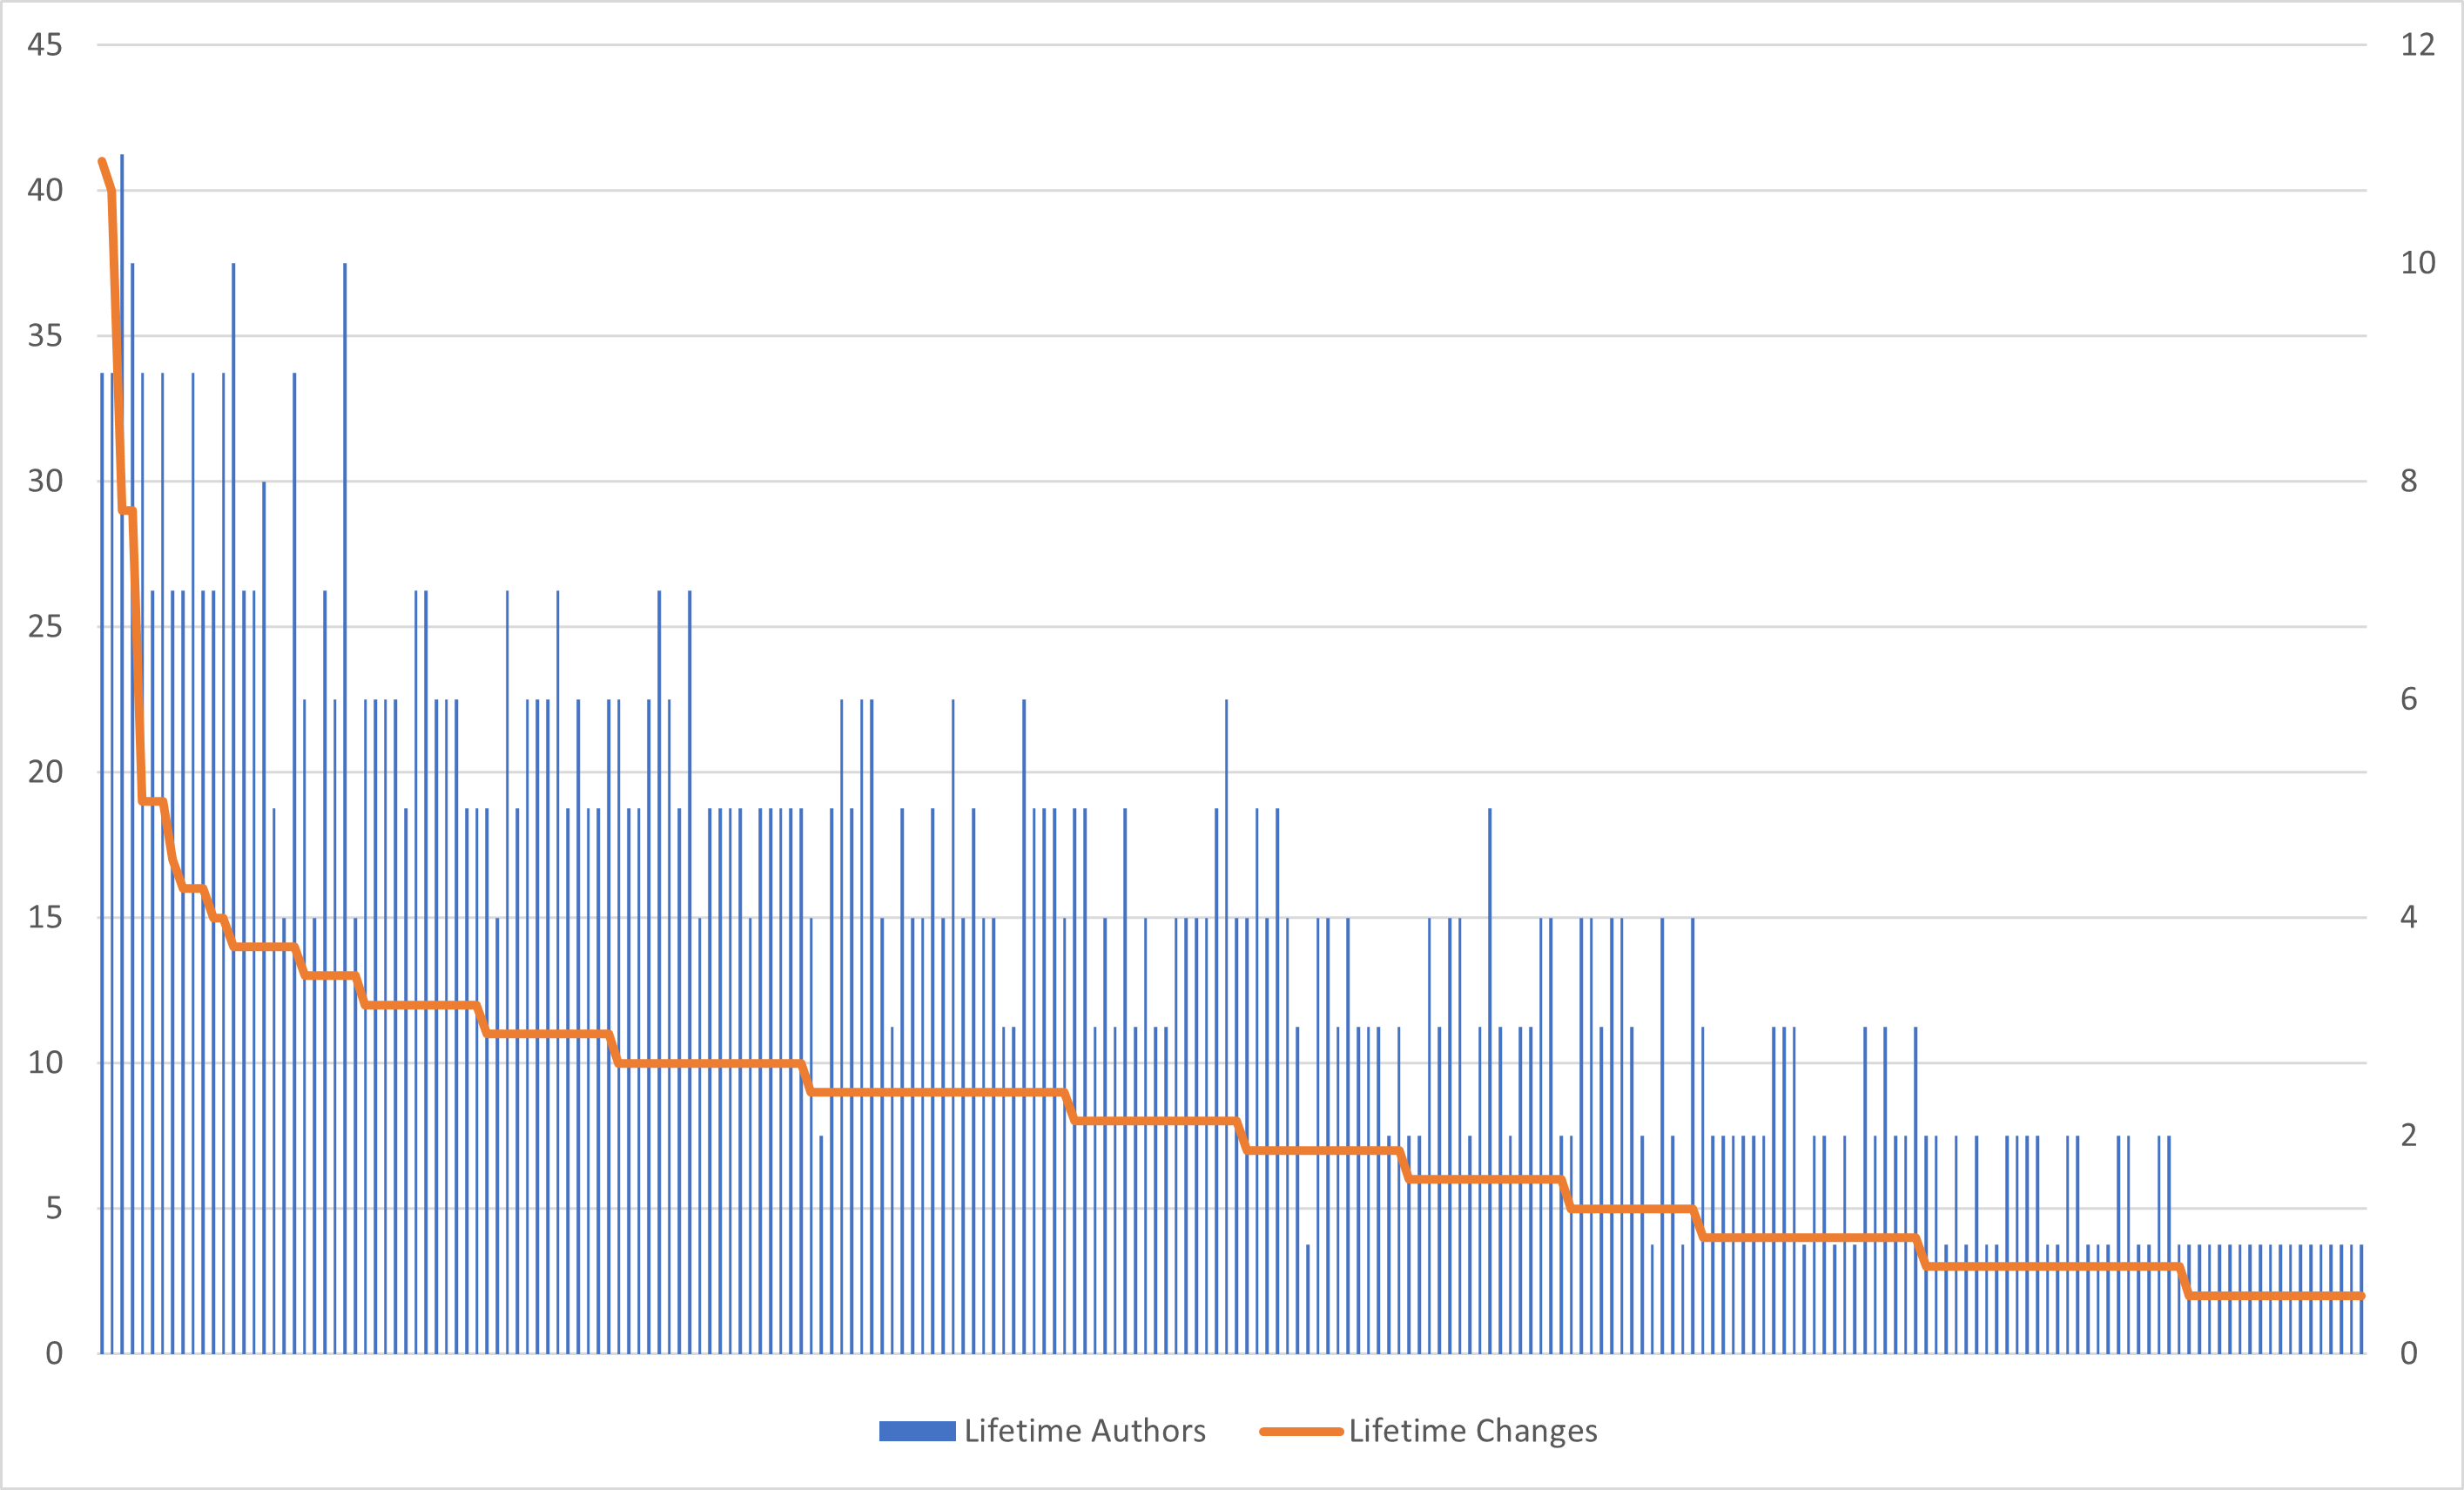
\includegraphics[width=1\textwidth]{images/moment/moment-2.20.5-changes.png}
    \caption{Moment.js 2.20.1-es kiadásában lévő fájlok módosítási számai}
    \label{fig:moment-2.20.1-changes}
\end{figure}

\begin{figure}[H]
    \centering
    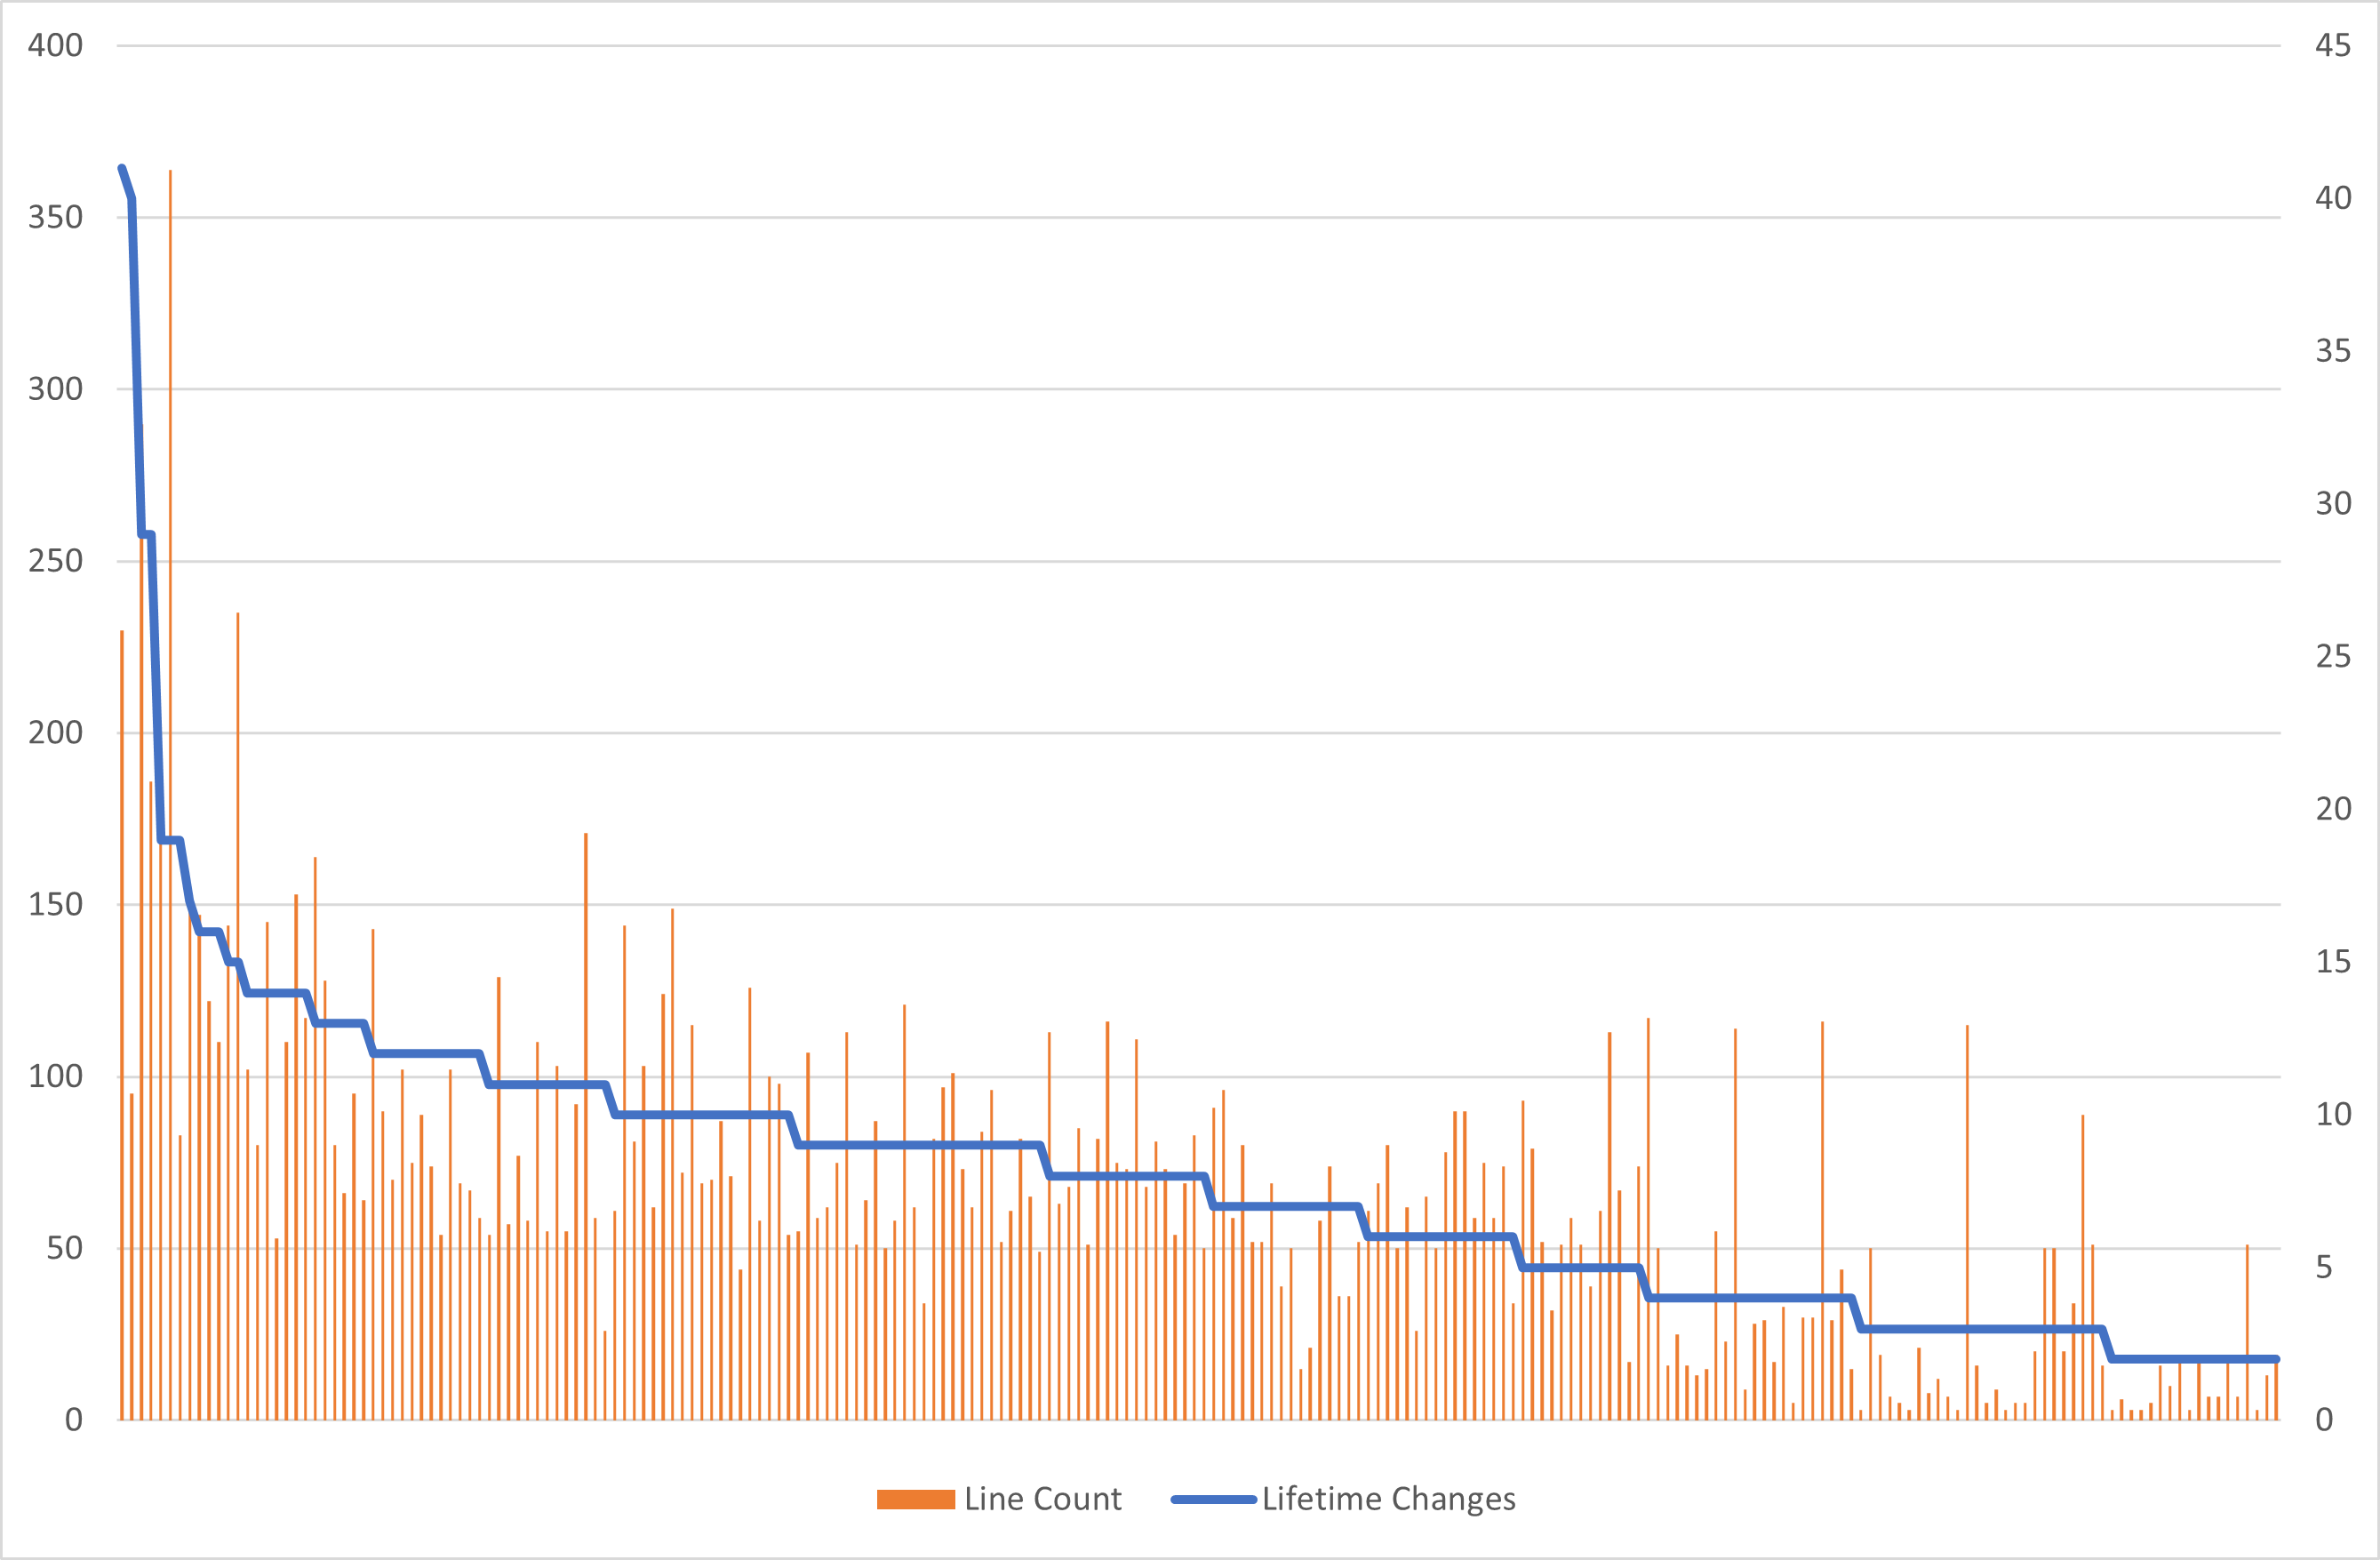
\includegraphics[width=1\textwidth]{images/moment/moment-2.20.5-auth.png}
    \caption{Moment.js 2.20.1-es kiadásában lévő fájlok módosítási számai és egyedi szerzőinek száma}
    \label{fig:moment-2.20.1-auth}
\end{figure}

\begin{figure}[H]
    \centering
    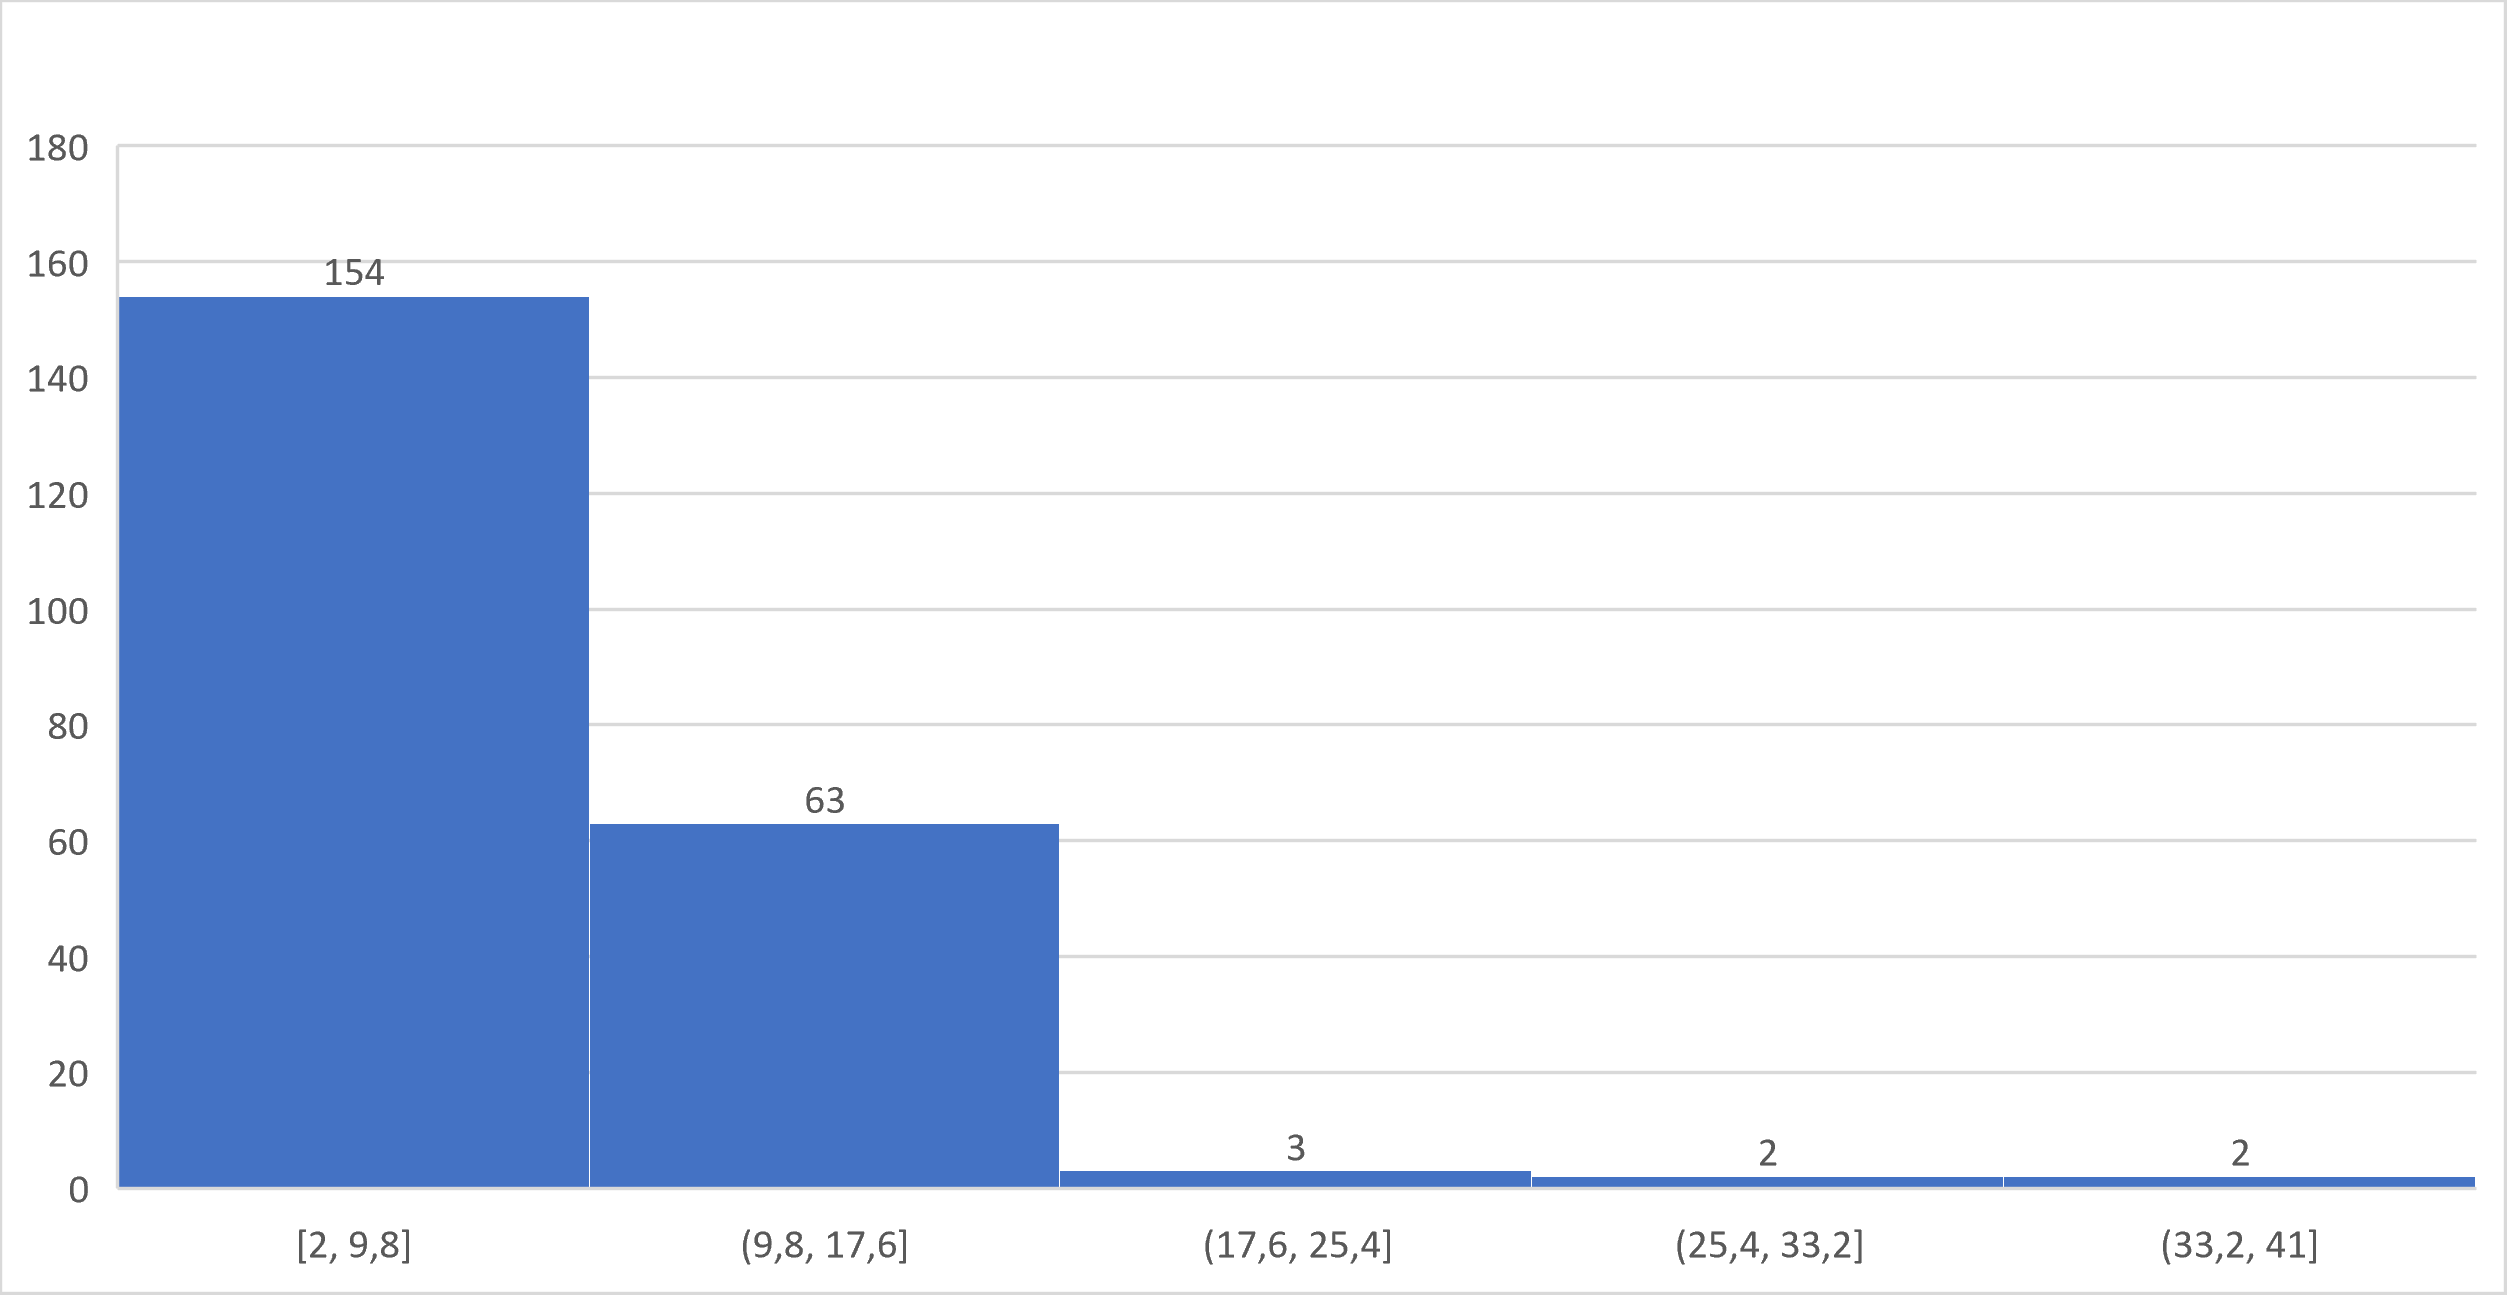
\includegraphics[width=1\textwidth]{images/moment/moment-2.20.5-hist.png}
    \caption{Moment.js 2.20.1-es kiadásában lévő fájlok módosítási számainak hisztogramja}
    \label{fig:moment-2.20.1-hist}
\end{figure}

Nézzük meg a moment.js végső kiadásának adatait. Mint látható a \ref{fig:moment-dev-changes} és \ref{fig:moment-dev-hist} ábrákról a kódbázis erőviszonyai nem változtak a végső kiadásban sem, megtartották azokat a trendeket, amikre a 2.20.1-es kiadás alapján számítanánk. A módosítási számok összehasonlítása a \ref{fig:moment-all-changes} ábrán látható: ebből is látszik, hogy a végső kiadás módosítási számai alapján rajzolt vonal közel van a 2.20.1-es adatokban látott trendekhez, de még a 2.10.5-ös verzióban látott viszonylag lapos kódbázis és a végső állapot közötti korreláció is viszonylag magas, 0,663.

\begin{figure}[H]
    \centering
    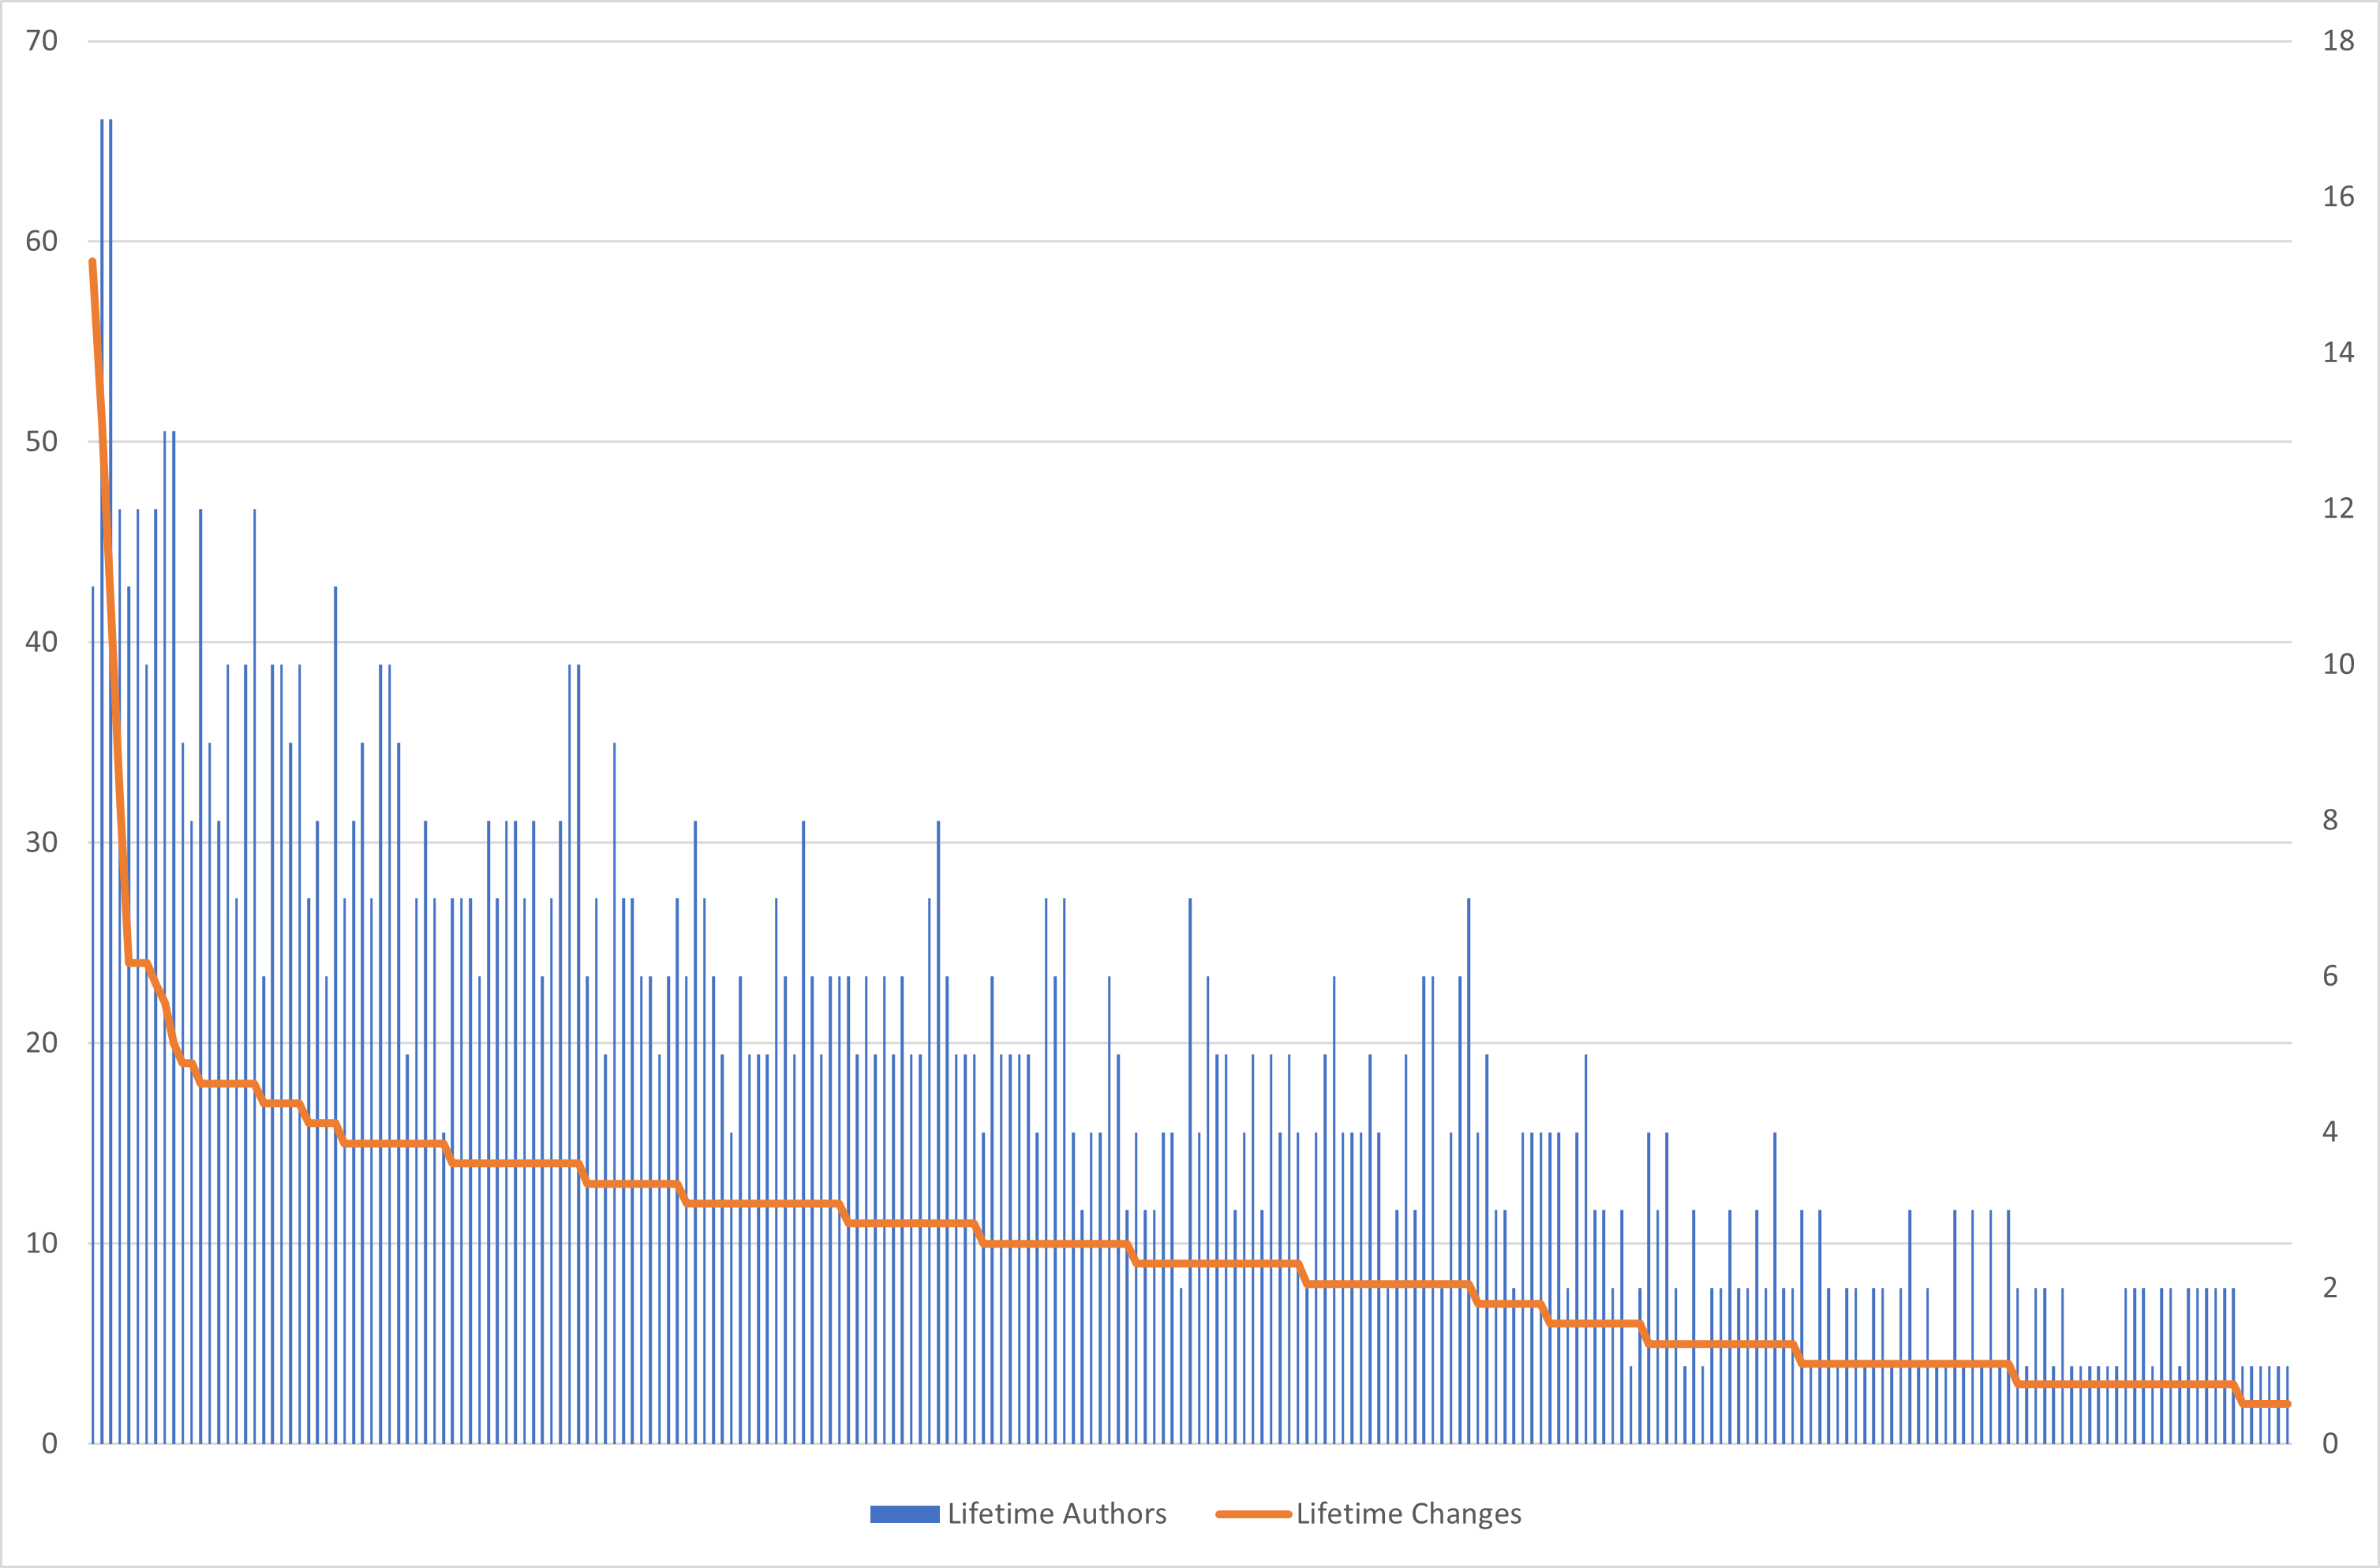
\includegraphics[width=1\textwidth]{images/moment/moment-dev-changes.png}
    \caption{Moment.js legfrisebb és egyben végső kiadásában lévő fájlok módosítási számai}
    \label{fig:moment-dev-changes}
\end{figure}

\begin{figure}[H]
    \centering
    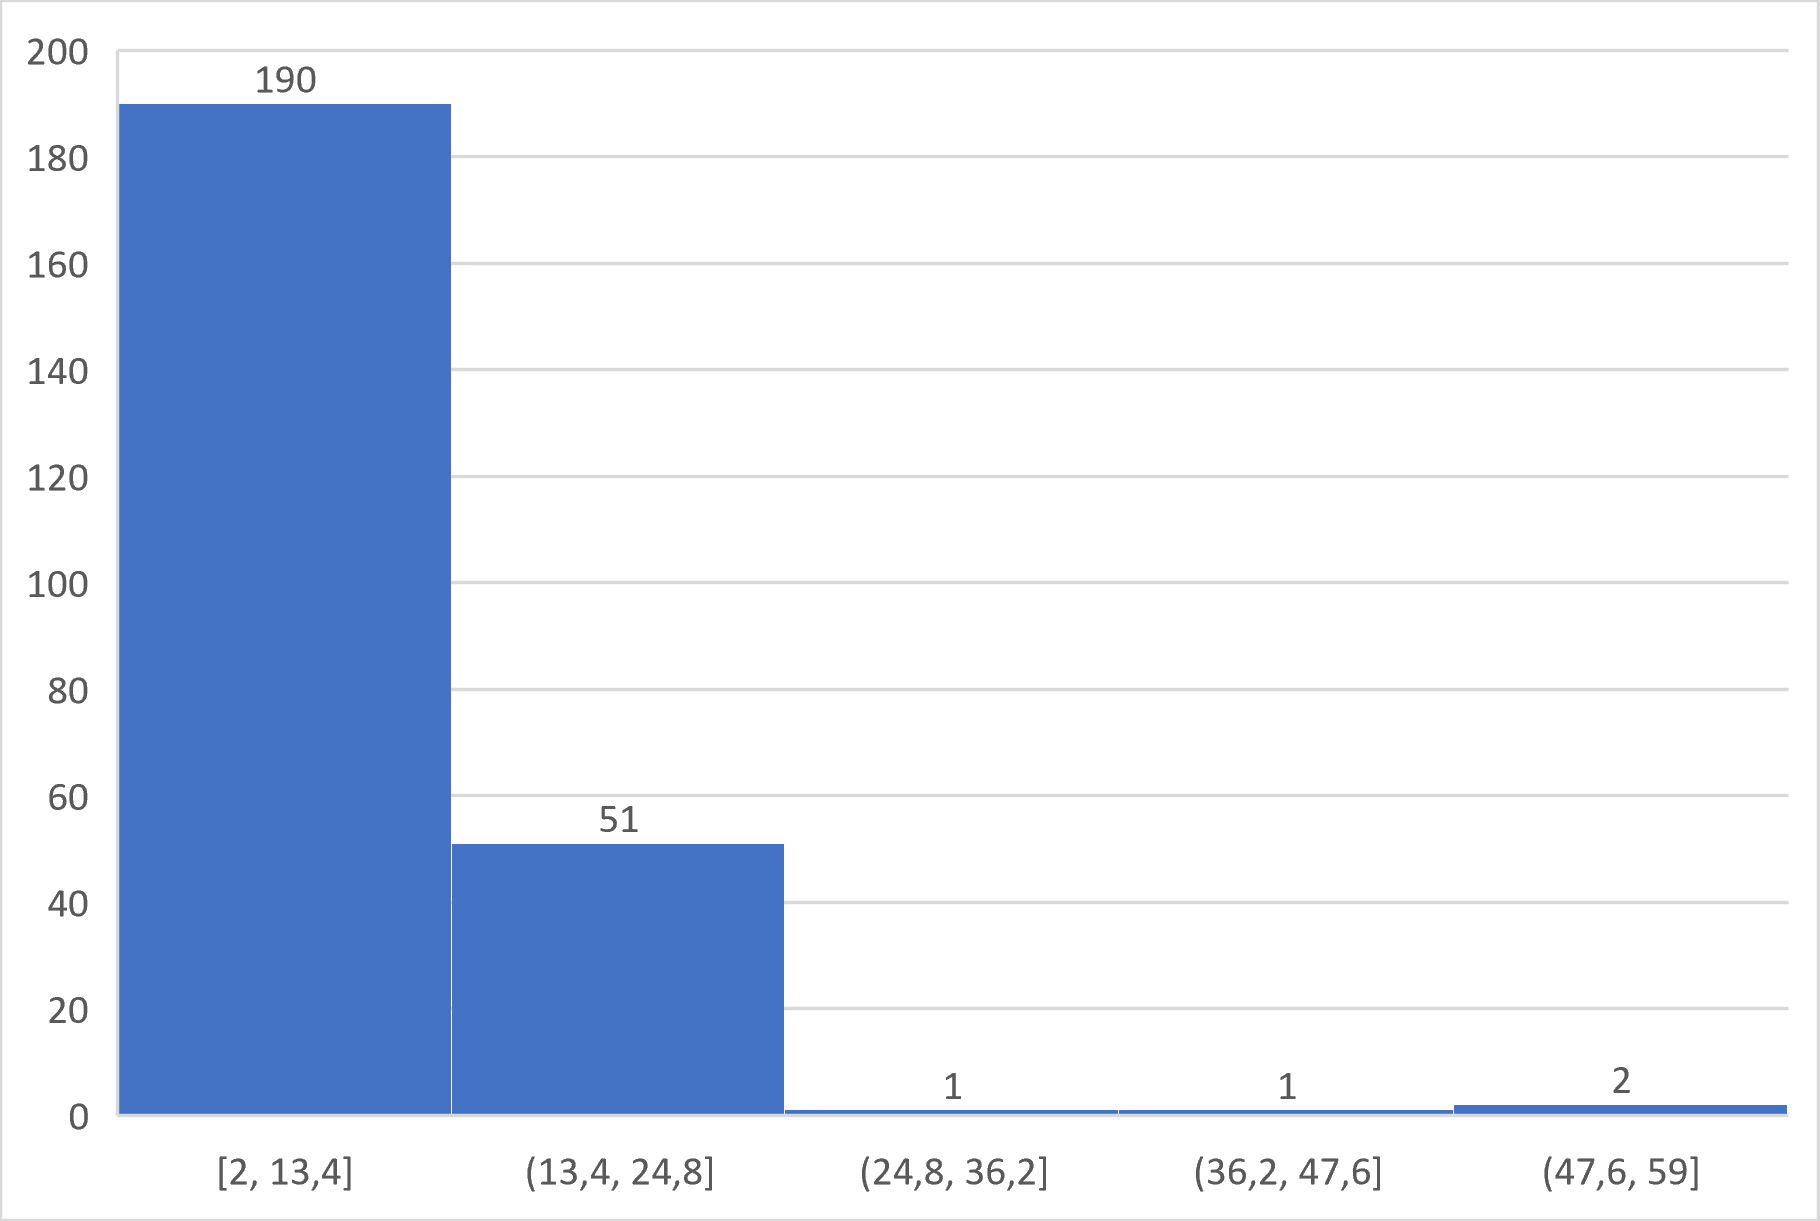
\includegraphics[width=1\textwidth]{images/moment/moment-dev-hist.png}
    \caption{Moment.js legfrisebb és egyben végső kiadásában lévő fájlok módosításinak hisztogramja}
    \label{fig:moment-dev-hist}
\end{figure}

\begin{figure}[H]
    \centering
    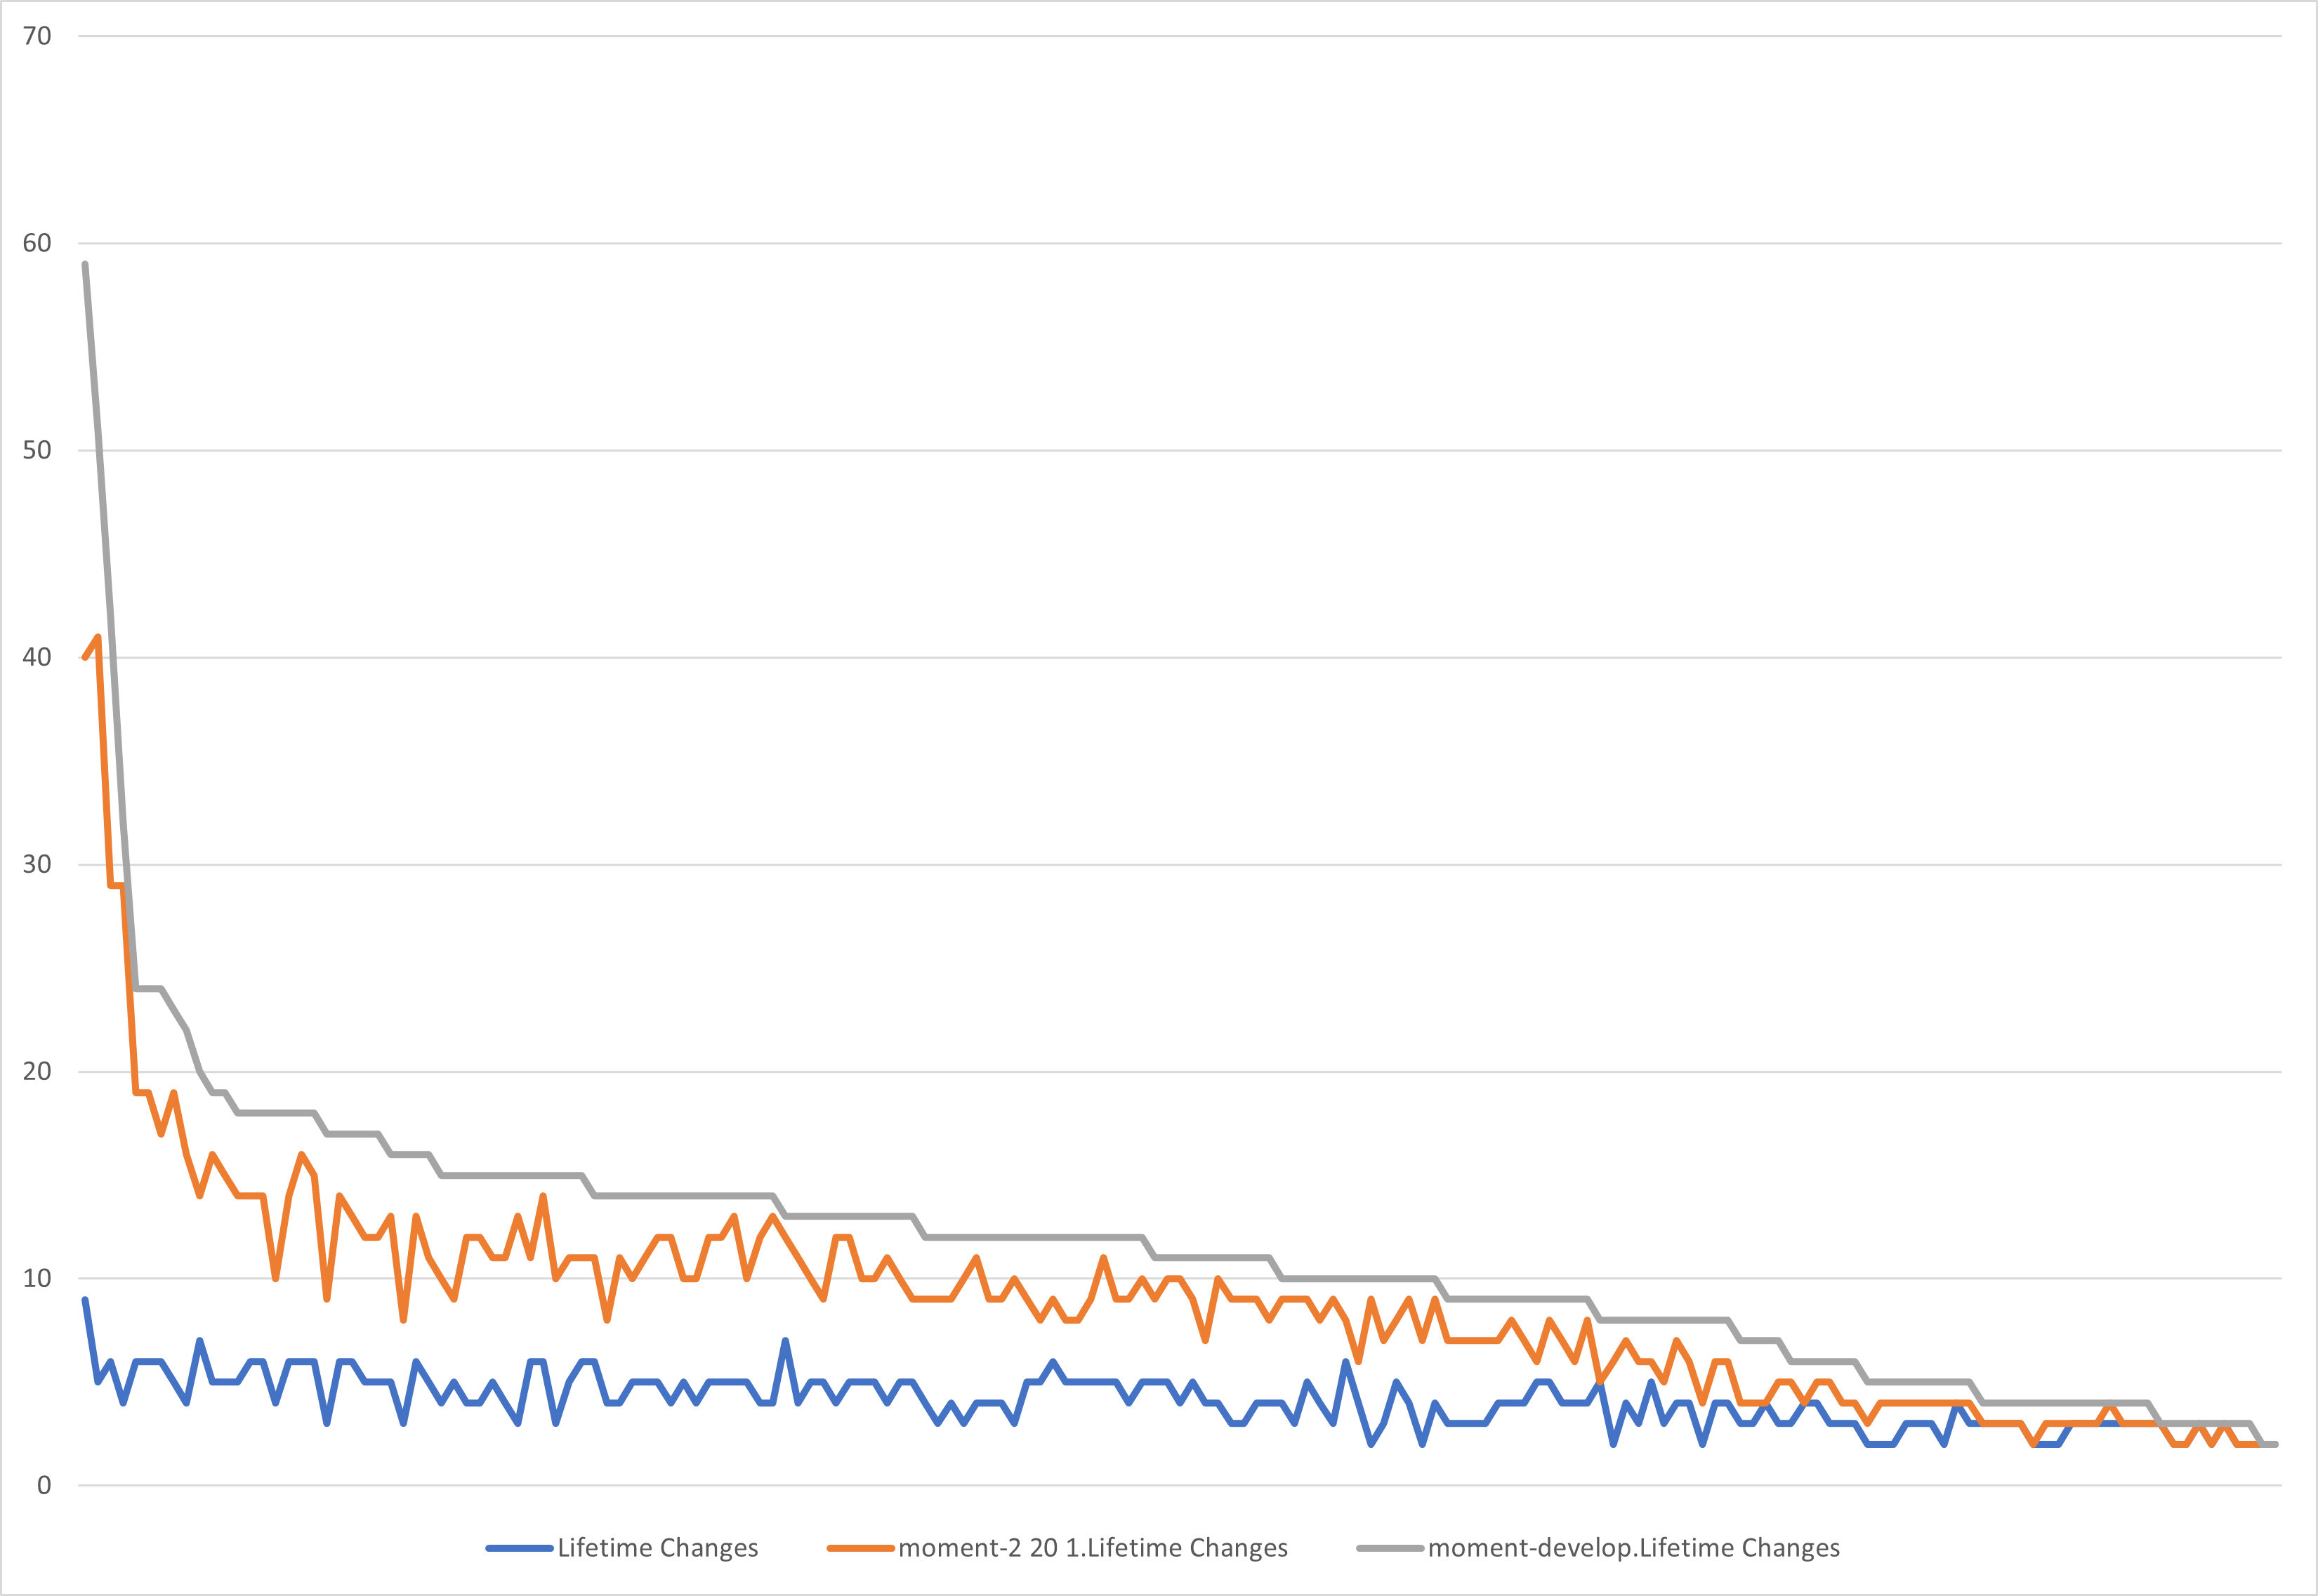
\includegraphics[width=1\textwidth]{images/moment/moment-all-changes.png}
    \caption{Moment.js módosítási számainak alakulása 2.10.5 és a végső kiadás között}
    \label{fig:moment-all-changes}
\end{figure}

Végül érdemes még röviden szót ejteni a coverage trendekről, mivel a moment.js reprezentálja az analízisek között az olyan kódbázist, ahol megkérdőjelezhető a tesztelés mennyisége és minősége.

Leszámítva az olyan anomáliákat, mint a \code{locale.js} és \code{ru.js} esetén eltűnő tesztek a 2.10.5-ös verziót követően, a kódbázis nagy részén

\begin{figure}[H]
    \centering
    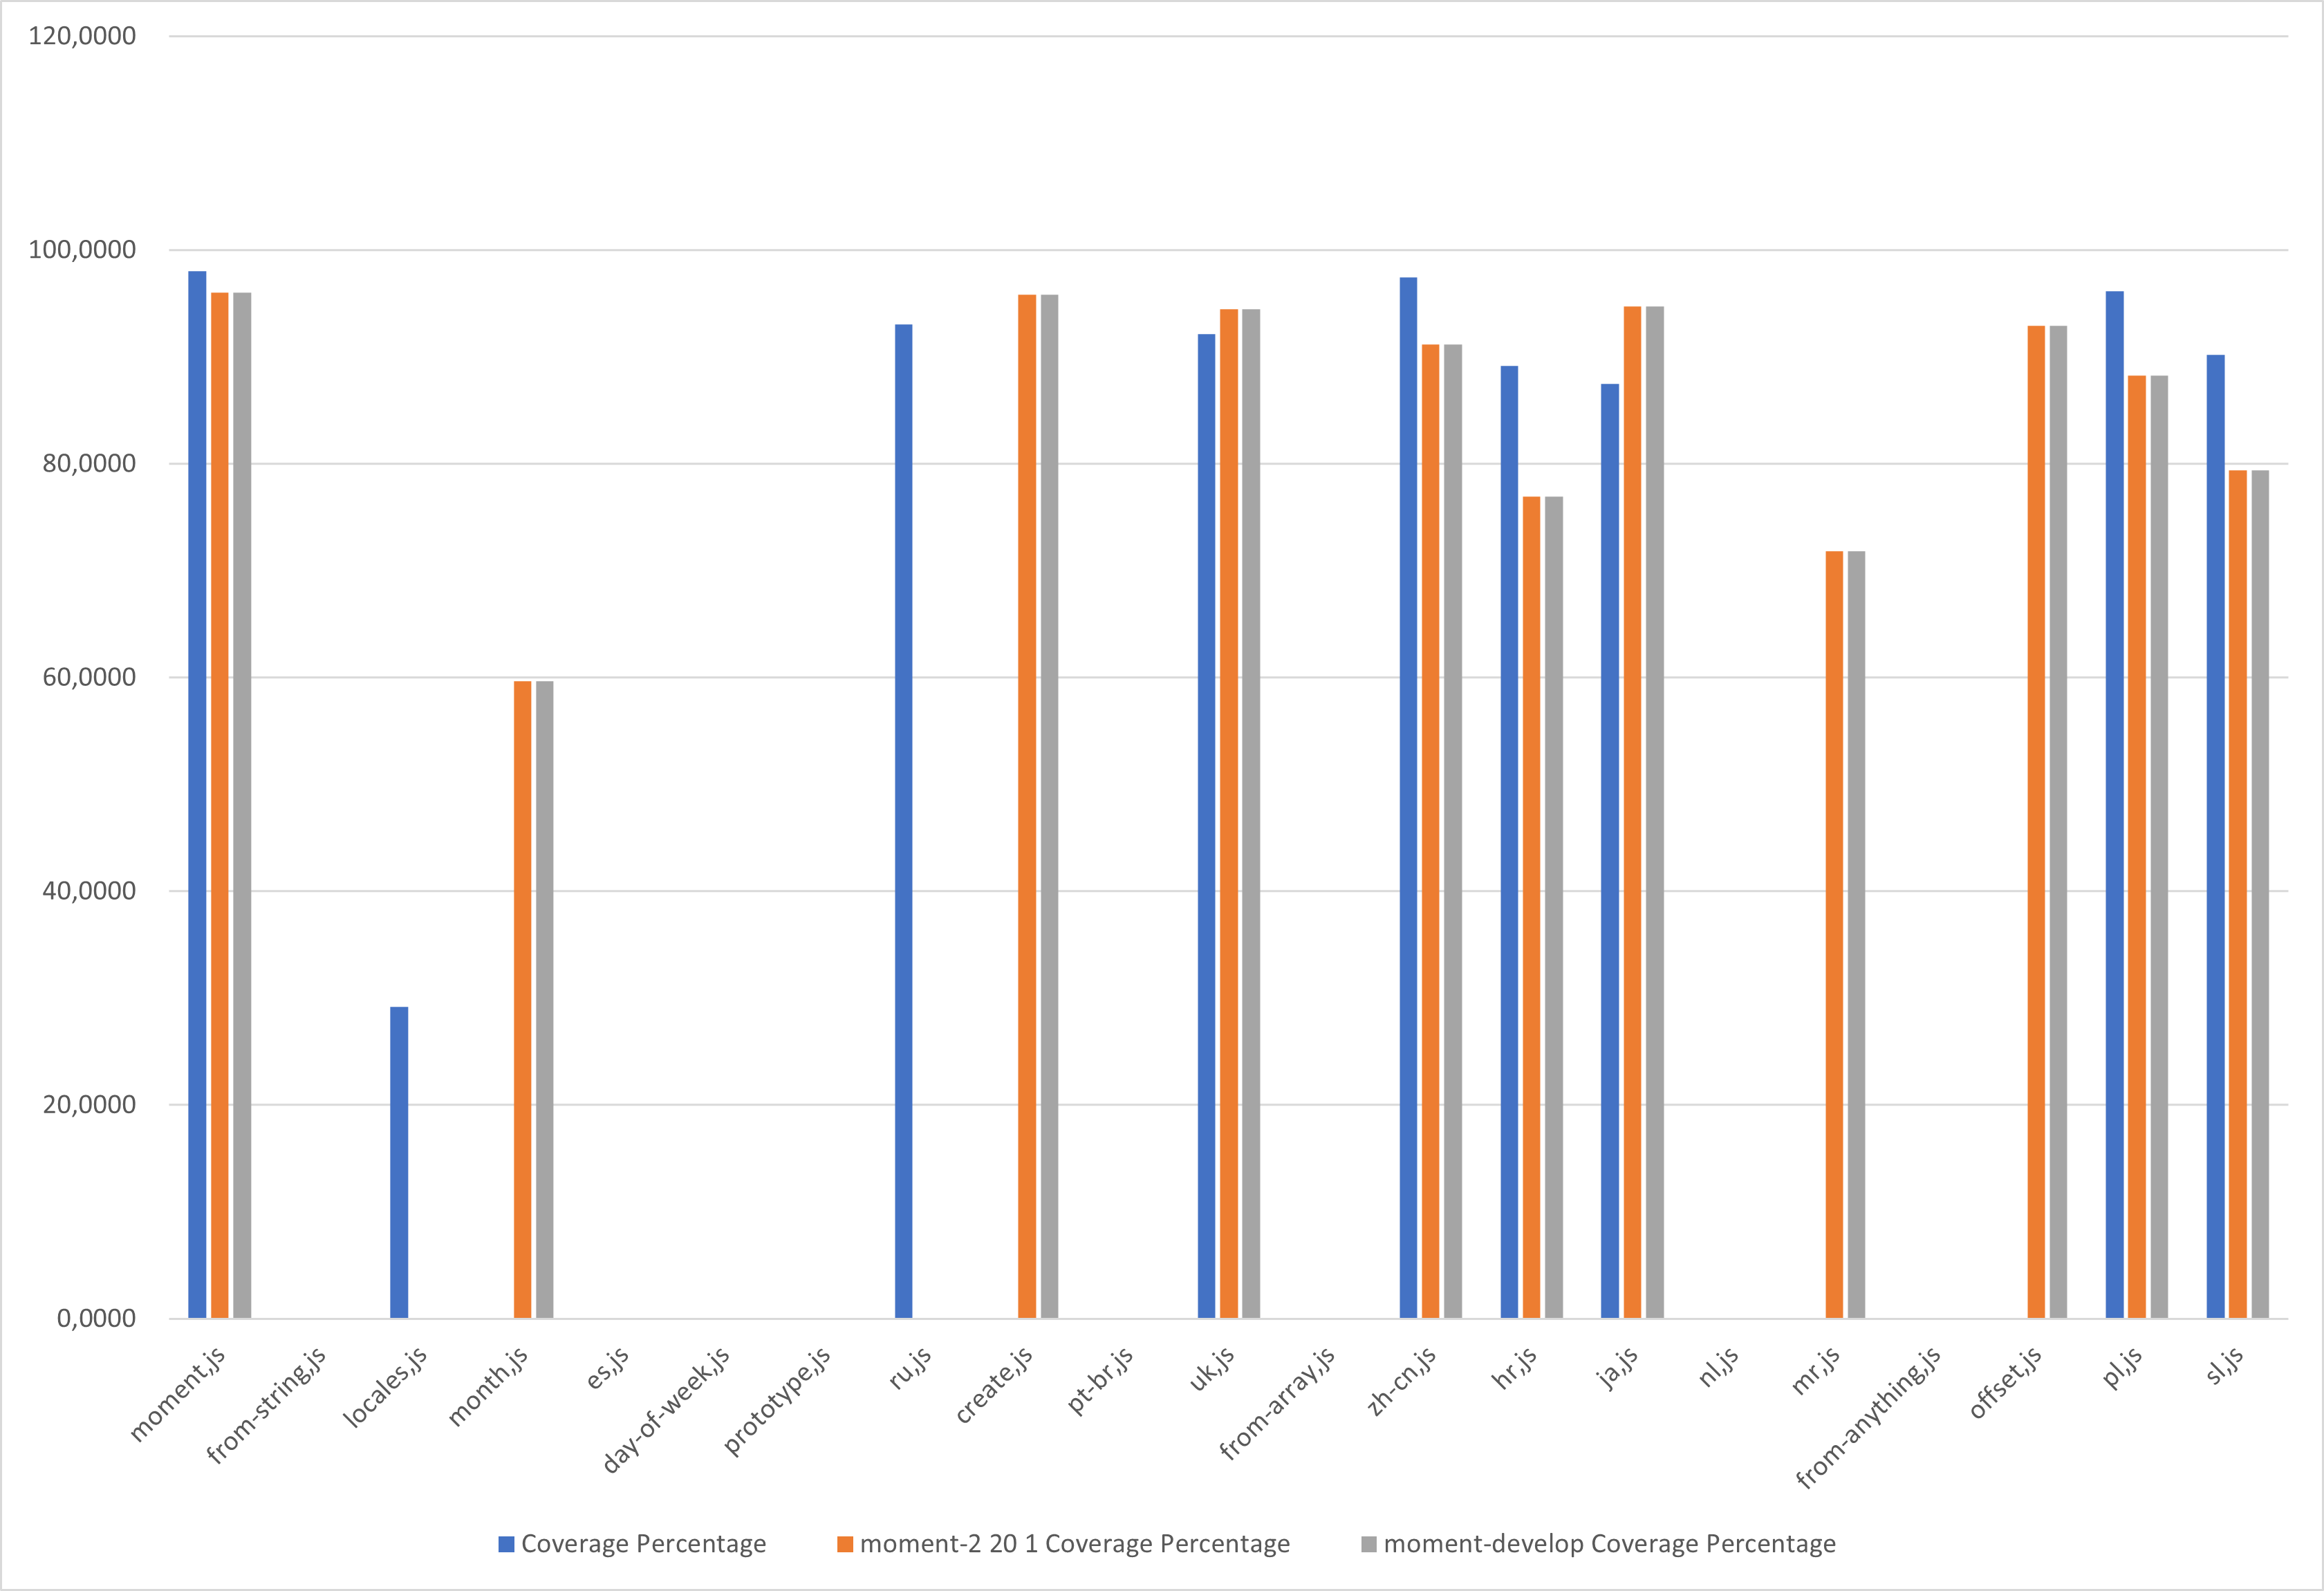
\includegraphics[width=1\textwidth]{images/moment/moment-all-coverage.png}
    \caption{Moment.js test coverage-ének alakulása 2.10.5 és a végső kiadás között}
    \label{fig:moment-all-coverage}
\end{figure}

\begin{figure}[H]
    \centering
    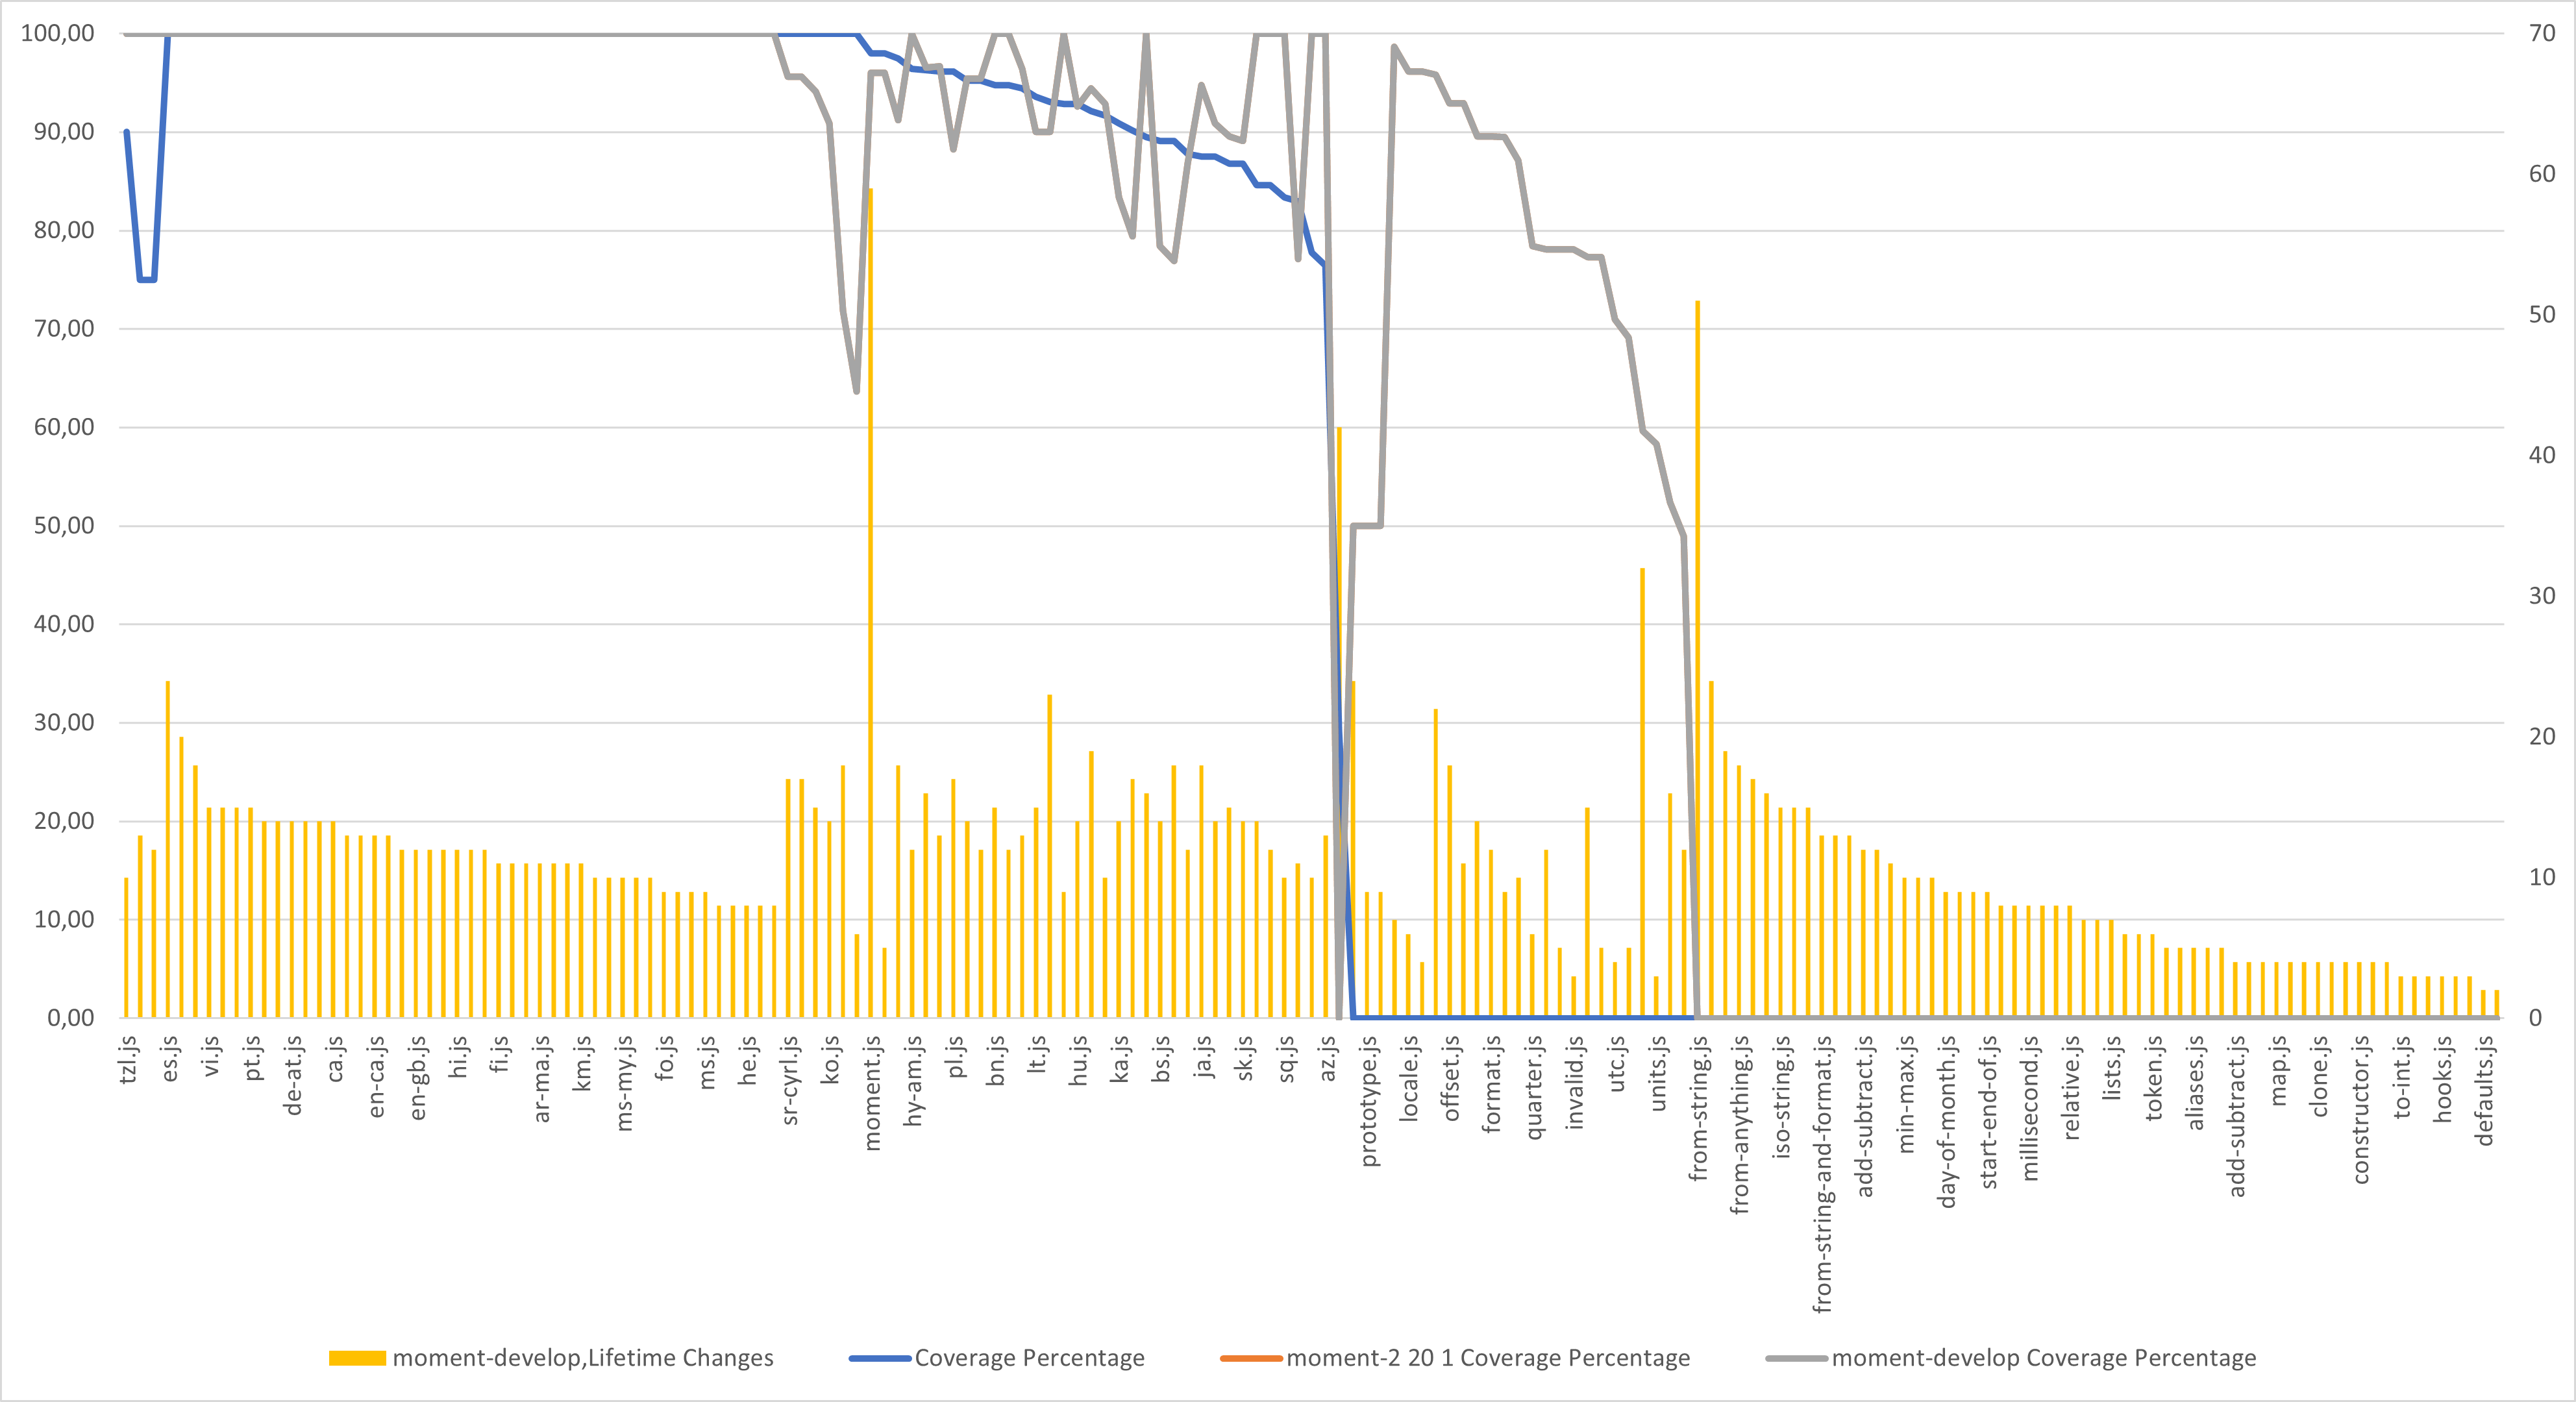
\includegraphics[width=1\textwidth]{images/moment/moment-all-coverage-full.png}
    \caption{Moment.js kódbázisának teljes coverage-e}
    \label{fig:moment-all-coverage-full}
\end{figure}

\section{React}

Utolsóként röviden a React\footnote{https://hu.reactjs.org/} kódbázisára fogunk kitérni. A React a vue-hoz hasonlóan egy webes, JavaScript-alapú frontend könyvtár. A React erősen épít a funkcionális programozásból ismert koncepciókra és a webes világ HTML-CSS-JS szegregációjától eltér a JSX formátumával, ami ezt a hármat ötvözi.

\lstset{language=JavaScript, caption={Egy egyszerű React komponens}}
\begin{lstlisting}
import React, { useState } from 'react';

function Example() {
    return (
        <div>
            <p>You clicked {count} times</p>
            <button onClick={() => setCount(count + 1)}>
                Click me
            </button>
        </div>
    );
}
\end{lstlisting}

Az analízis rövidségének két oka van:
\begin{enumerate}
    \item A react kódbázisa több nagy refactor-on esett át, ami jelentősen megnehezíti a különböző verziók közötti kapcsolatok kialakítását. A snapshot-okat általában a különböző fájlok elérési útvonalain lehet csak összekapcsolni, mert a fájlok nevei nem egyediek, viszont az elérési útvonalak változása miatt csak egy nagyon kis szeletét lehetne megvizsgálni a projektnek
    \item A régebbi react kiadásokra nem lehet coverage report-okat generálni, mert a projekt egyik histórikus függősége egy az egyben el lett távolítva az npm-ről biztonsági okokból
\end{enumerate}

Ennek ellenére a react kódbázisa különösen érdekes lesz, mert egy olyan jelenséget produkál, amit a vue és a moment.js nem.
Elsőként nézzük a React 14-es és 15-ös verziójának a legtöbbet módosított fájljait a \ref{fig:react-14-15-changes} ábrán. Eddig egyelőre nem látszik semmi különös, nagyrészt hasonló értékeket és mintákat látunk, mint a vue és a moment esetében.

\begin{figure}[H]
    \centering
    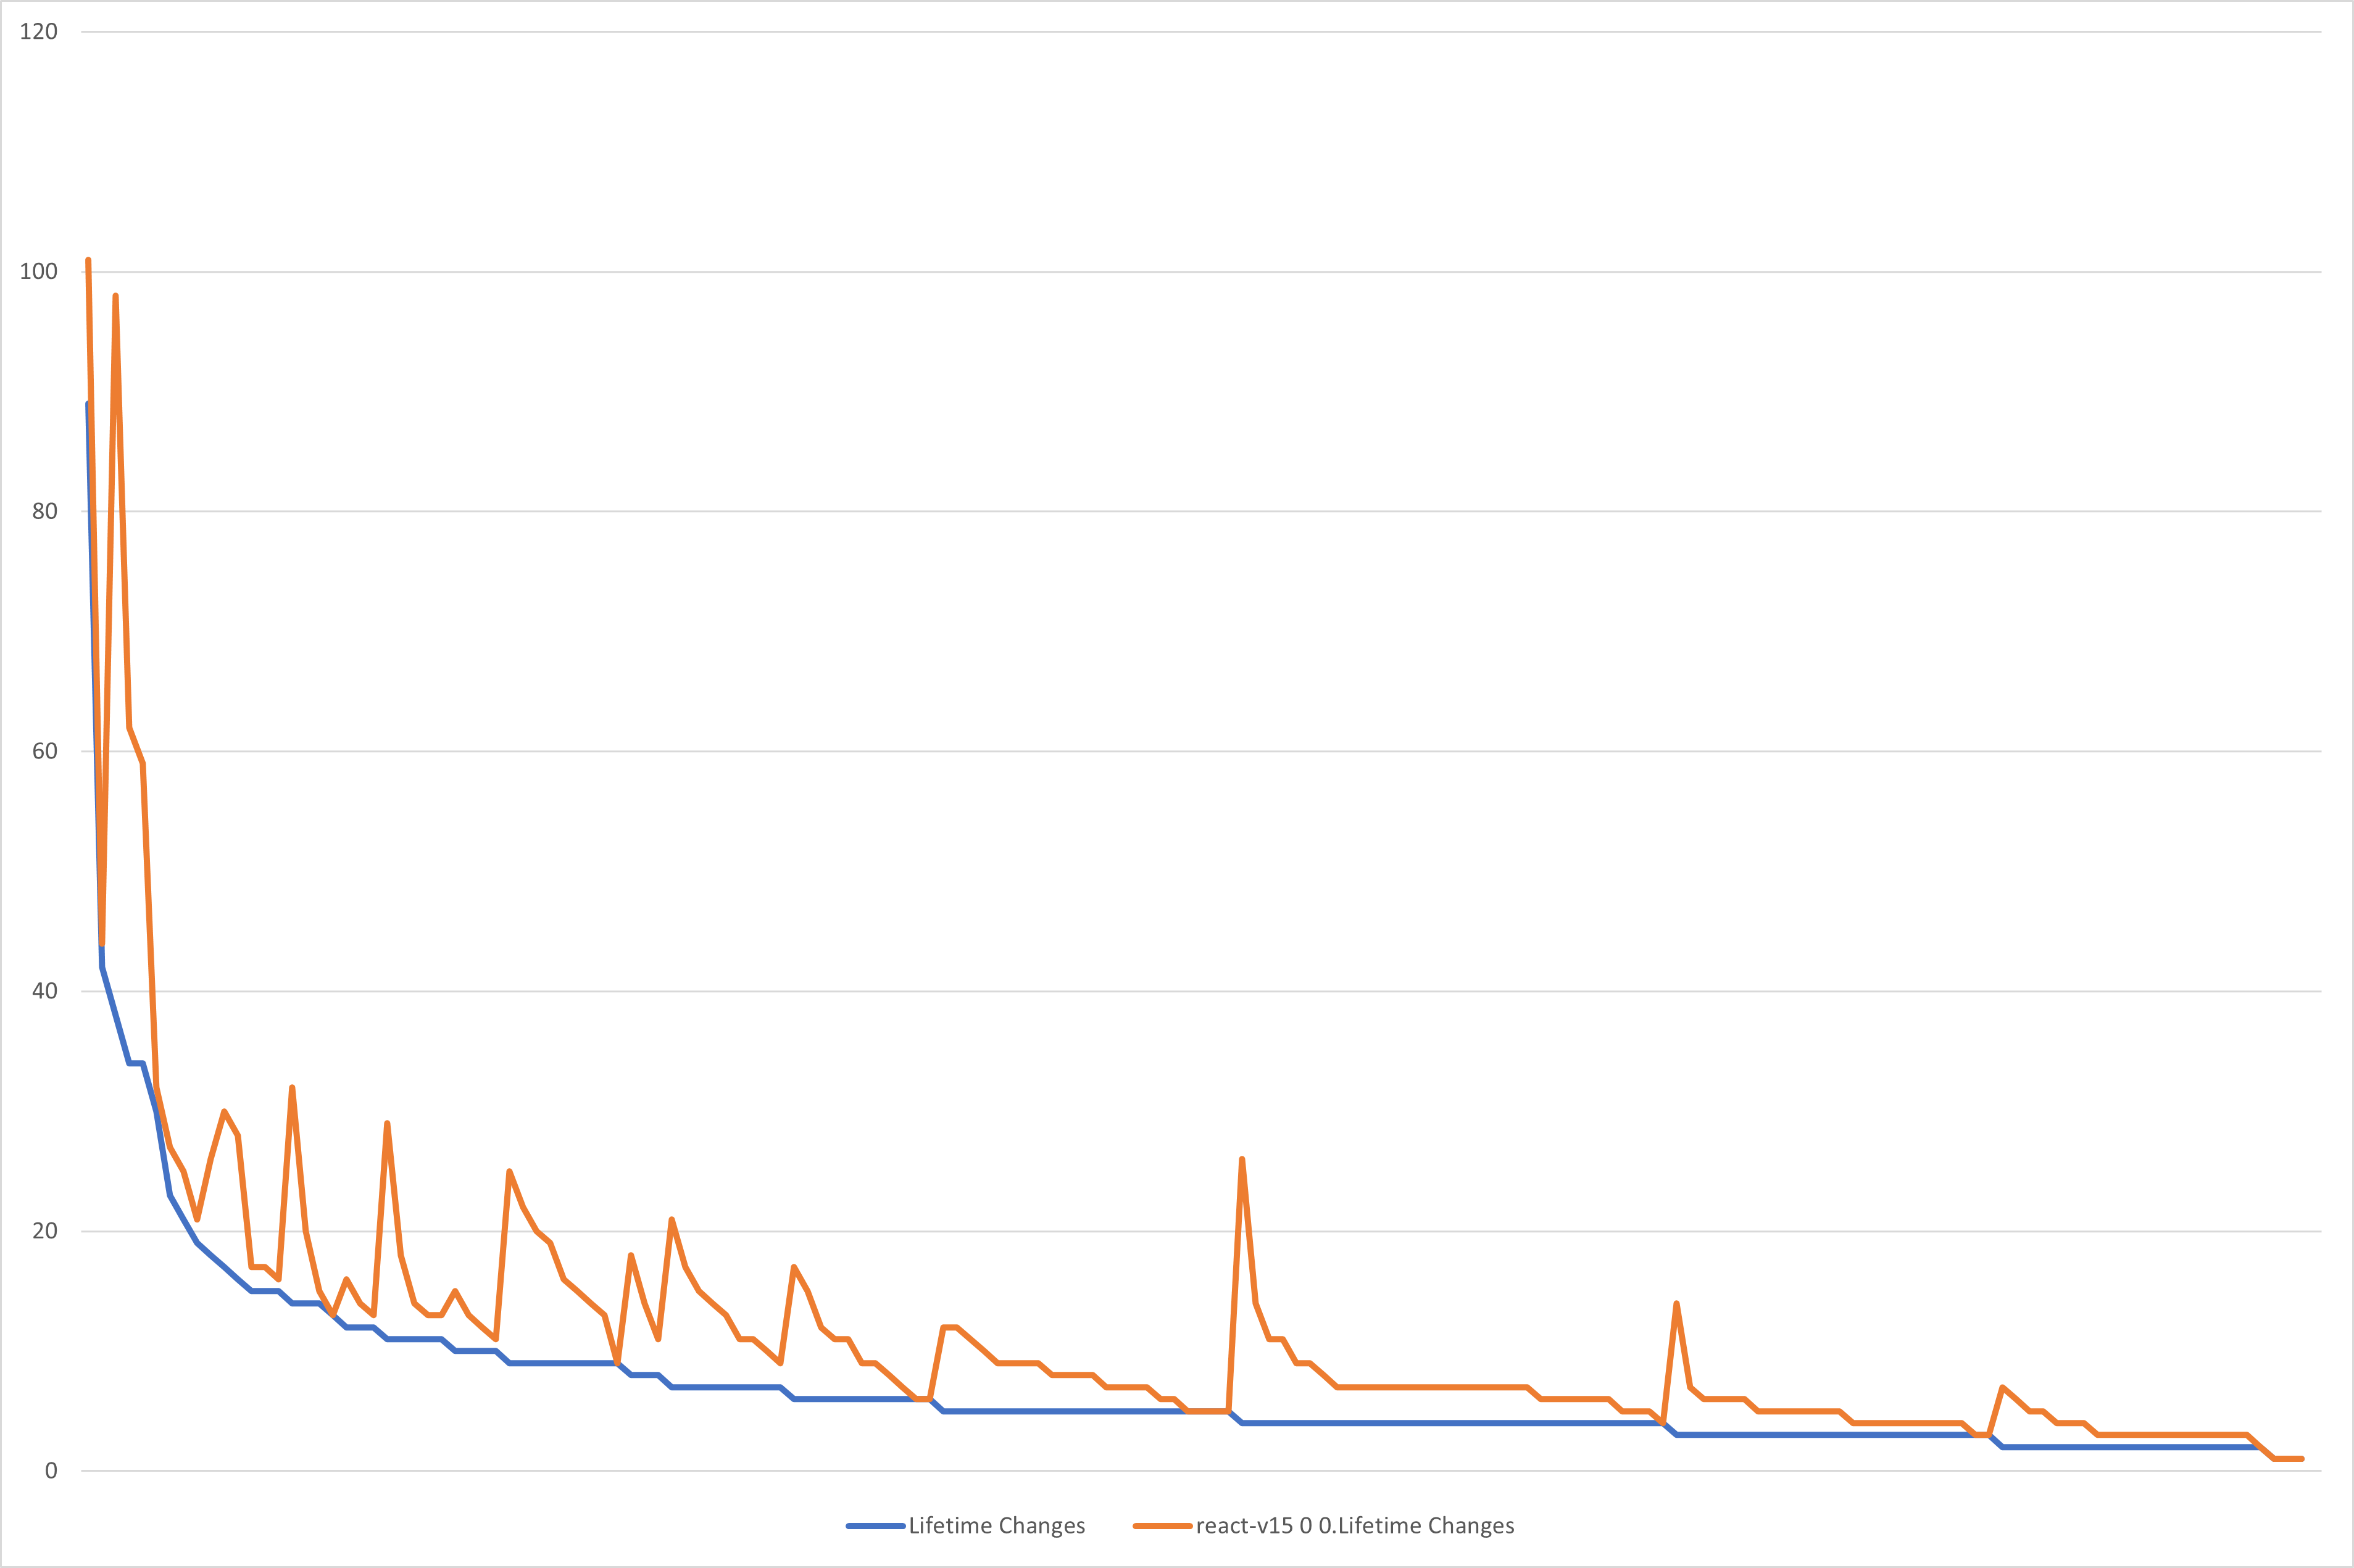
\includegraphics[width=1\textwidth]{images/react/react-14-15-changes.png}
    \caption{A React 14-es és 15-ös verziójának módosítási számai}
    \label{fig:react-14-15-changes}
\end{figure}

Vessünk azonban egy pillantást a \ref{tab:react-all-changes} táblázatra, amiben 16-os verzióban legtöbbet változtatott fájlok szerepelnek a histórikus módosítási adatokkal. Mint látható, a top 10-ben 9 olyan fájl van, amik nem léteztek a 16-os verziót megelőzően. Ez egy kis magyarázatra szorul.

A React a 16-os kiadásban egy teljes új renderelő architektúrára váltott, ami Fiber\footnote{https://reactjs.org/blog/2017/09/26/react-v16.0.html\#new-core-architecture} kódnéven futott. Nyilvánvalóan egy frontend framework legkritikusabb része a DOM rendering, amit gyakorlatilag alapjaitól írtak újra a React fejlesztői. Ugyan ez a változtatás a 16-os verzióban került be az éles kódbázisba, egy párhuzamos branch-en akkor már évek óta aktív fejlesztés alatt állt.

Az eddigi megfigyelések azt mutatták, hogy amikor egy kódbázis elindul egy bizonyos irányba, akkor a korai módosítási minták medrében folyik a fejlesztés a projekt élete során. A react azonban jó példa arra, hogy ez nem feltétlenül igaz: ha a projekt új architektúrára vált, akkor ki lehet kerülni az előre lefektetett mintákat.

Ebben az esetben azonban azonban ez az új architektúra hiába cseréli le a régi, sokat módosított fájlokat, ahogy az \ref{fig:react-all-changes} ábrán látszik a Fiber architektúra pontosan ugyanazt a mintát mutatja, hiába teljesen új kód. Ez természetesen ahogy korábban a code smell-eknél tisztáztuk nem feltétlenül gond, hiszen a projekt korai hibáit javító, új központi architektúra objektíven tud emelni a projekt színvonalán.

\begin{table}[h]
    \centering
    \begin{tabular}{l|l|l|l}
        Filename                    & v14 & v15 & v16 \\ \hline
        ReactFiberScheduler.js      & 0   & 0   & 187 \\
        ReactFiberBeginWork.js      & 0   & 0   & 161 \\
        ReactFiberReconciler.js     & 0   & 0   & 114 \\
        ReactChildFiber.js          & 0   & 0   & 102 \\
        ReactFiberCompleteWork.js   & 0   & 0   & 95  \\
        ReactFiber.js               & 0   & 0   & 87  \\
        ReactFiberCommitWork.js     & 0   & 0   & 78  \\
        ReactDOMFiberComponent.js   & 0   & 0   & 77  \\
        ReactFiberClassComponent.js & 0   & 0   & 73  \\
        ReactCompositeComponent.js  & 34  & 62  & 63  \\
        ReactElement.js             & 17  & 30  & 55  \\
        ReactFiberUpdateQueue.js    & 0   & 0   & 52  \\
        DOMPropertyOperations.js    & 11  & 29  & 49  \\
        ReactElementValidator.js    & 15  & 17  & 49  \\
        HTMLDOMPropertyConfig.js    & 14  & 32  & 48  \\
        ReactFiberContext.js        & 0   & 0   & 44  \\
        ReactDOMComponent.js        & 38  & 38  & 38
    \end{tabular}
    \caption{A React 16-os kiadása}
    \label{tab:react-all-changes}
\end{table}

\begin{figure}[H]
    \centering
    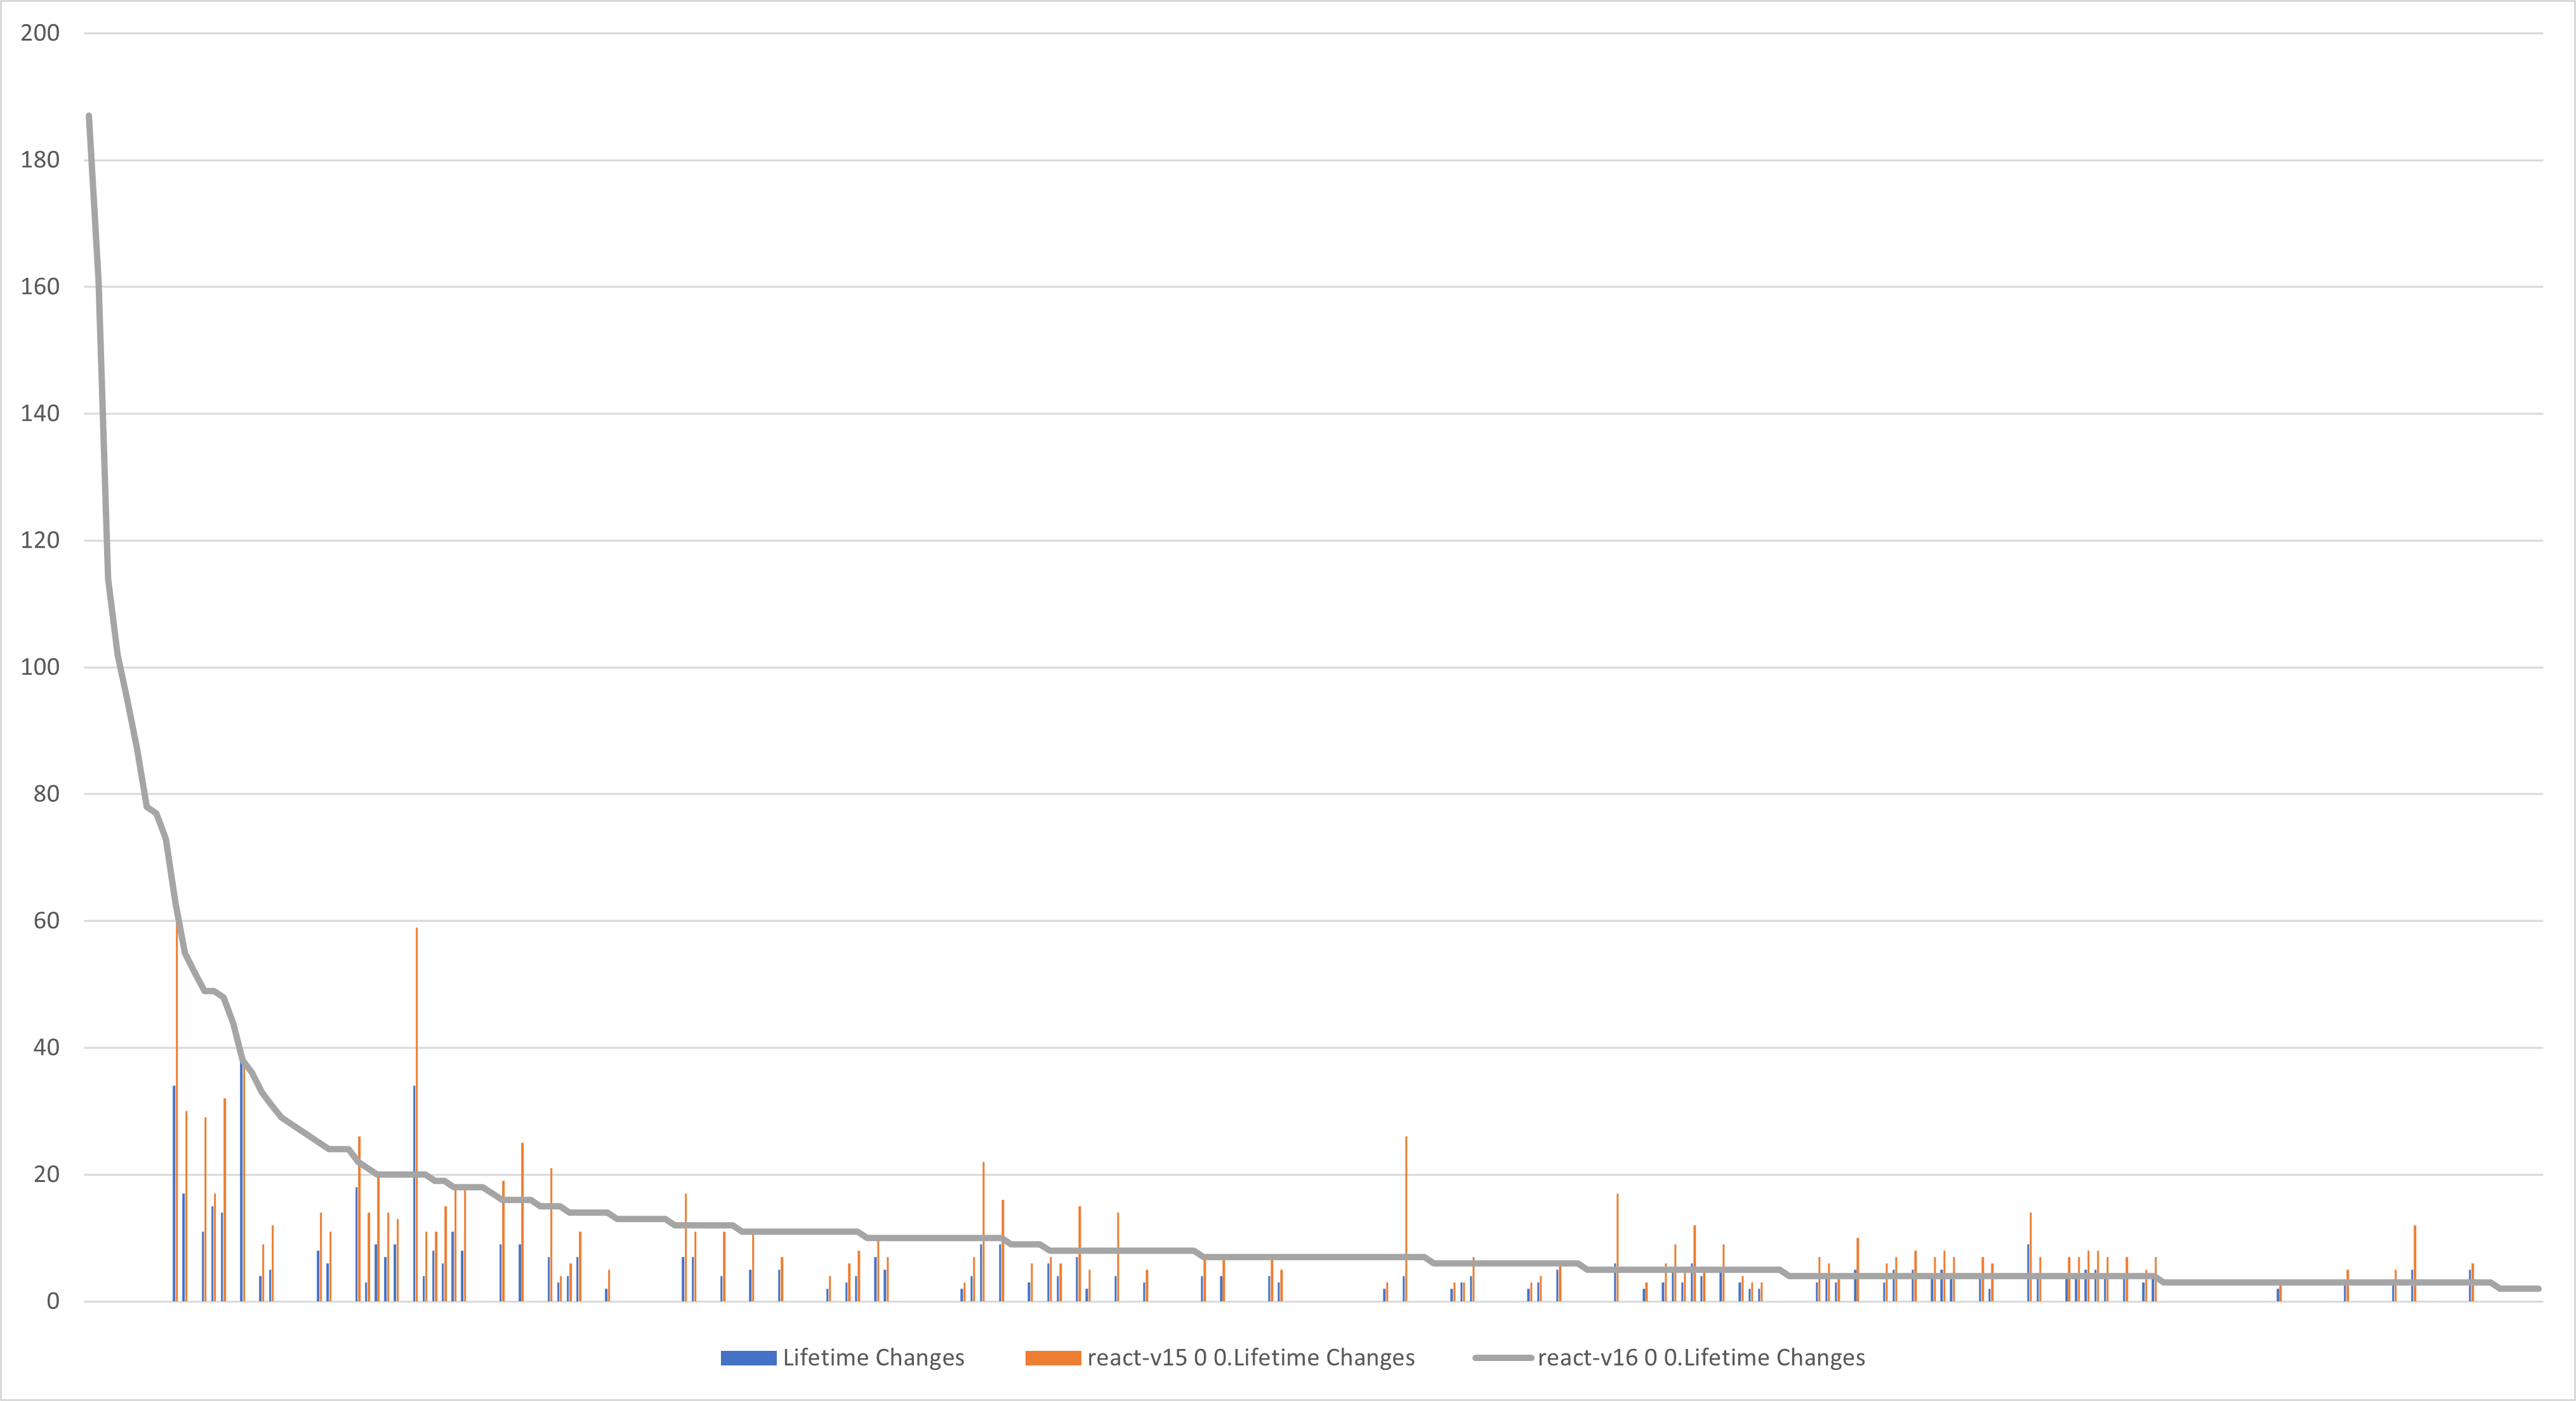
\includegraphics[width=1\textwidth]{images/react/react-all-changes.png}
    \caption{A React teljes kódbázisa a 14-es, 15-ös és 16-os kiadásokban}
    \label{fig:react-all-changes}
\end{figure}
\cleardoublepage

\chapter{Összegzés}
\label{ch:sum}

\section{Eredmények}

A cél ebben a diplomamunkában az volt, hogy néhány nyílt forráskódú projekteken végezzünk el git statisztikai és coverage vizsgálatot és nézzük meg ezeket egyrészt külön-külön, másrészt olyan szempontból is, hogy milyen kapcsolatban állnak egymással.

A Vue és a Moment projekteken végzett analízis jó példája volt annak, amire \textit{Khohm et al.}\cite{khomh} is rámutatott: a kódbázisokban képesek kialakulni módosítási gócpontok, amik a projekt élettartama alatt konzisztensen ezt a mintát fogják mutatni. Láttuk azt is, amit \textit{M. Tufano et al.}\cite{codeSmells} állított, miszerint az ilyen módosítási gócpontok a közhiedelemmel ellentétben nem a kódbázis evolúciója során jönnek létre, hanem általában már az alapkövek lefektetésekor jelen vannak.
A Vue jó példa volt arra is, hogy önmagában egy gócpont szétbontása nem feltétlenül oldja meg a problémát, hiszen a \code{compile.js} egy teljes refactor után a következő kiadásban két külön gócpontként tért vissza.

Megvizsgáltuk továbbá a coverage és a módosítási gócpontok közötti relációt is. Ugyan három projekt analízise alapján ezt nem lehet konklúzívan kijelenteni, de a megfigyelések szerint a coverage, ahogy nem kódminőségi metrika, úgy nem moderáló faktor a módosítási gócpontok kialakulásában. A vue esetében látható volt, hogy a leggyakrabban módosított fájlok coverage-e 100\% volt a projekt teljes életciklusa során, hiába növekedtek verzióról verzióra. Egy kicsit bíztatóbb metrika volt azonban az, hogy a coverage a látottak alapján nem csökken ezeken a gócpontokon a növekedésük során.

A React kódbázisán láttunk egy olyan jelenséget is, ami különösen érdekes volt. A központi rendering pipeline, ami a React legnagyobb gócpontját képezte teljesen le lett cserélve az egyik kiadásban, de gyakorlatilag az első pillanattól kezdve ugyanazokat a mintákat mutatta az új renderer, mint a korábbi, hiába volt teljesen új kód.

Milyen tanulságokat vonhatunk le ezekből az eredményekből?

Az első az, hogy a git és úgy általánosságban a verziókezelők statisztikáinak analízise valóban egy jó eszköz, ha objektíven meg szeretnénk vizsgálni egy kódbázis állapotát. Ugyan az, hogy felismerünk egy fájlt, mint módosítási gócpont, az nem garantálja, hogy az a fájl code smell, vagy code smell-eket tartalmaz, de gyanakvásra adhat okot. Továbbá saját projekten alkalmazva ezt a vizsgálatot tovább lehet vinni, hiszen az analízis alkalmazható egy fájlra a sorok szintjén is, ami mélyebb problémákra is képes rávilágítani.

A második tanulság számomra az, hogy a coverage valóban nem alkalmazható minőségi metrikaként, hiszen semmilyen korrelációt nem mutatott sem maga a coverage, sem annak a változása a gócpontok egyik metrikájával sem.

\section{További kutatási lehetőségek}

Az analízisikhez szükséges adatok előkészítésénél világossá vált, hogy ugyan a program kiválóan működik, amikor egy specifikus verzió snapshot-ját készítjük el, a mélyebb analízishez több snapshot elkészítésére van szükség, amiket utána a fájlok nevei, elérési útjai és git történetük alapján össze kell kapcsolni. Ezeket az összekapcsolásokat, ahogy én is tettem, Excel-ben is el lehet végezni, azonban ez a megoldás egyrészt nem skálázódik túl jól, másrészt a git történet alapján való összekapcsolás így gyakorlatilag lehetetlen. Továbbá ha a program képes lenne összekapcsolni snapshot-okat, akkor az így generált adatok adatbányászati szempontból nagyon érdekesek lennének.

A program fejlesztésén túl érdekes lenne továbbá a prezentált analízis használata olyan ipari projekteken, amiken egyrészt generálható histórikus coverage adat, másrészt pedig nem feltétlen JavaScript-ben lettek fejlesztve, hiszen a platform és nyelv választása valamilyen szinten torzítja az itt látott analíziseket.

\cleardoublepage

\addcontentsline{toc}{chapter}{\biblabel}
\hbadness 10000 \printbibliography[title=\biblabel]
\cleardoublepage

\listoftables
\cleardoublepage

\listoffigures
\cleardoublepage

\end{document}
